\documentclass[a4paper]{article}


% Esto es para que el LaTeX sepa que el texto está en español:
\usepackage[english]{babel}
\selectlanguage{english}

% Esto es para poder escribir acentos directamente:
\usepackage[utf8]{inputenc}
\usepackage[T1]{fontenc}

%% Pa meter links y refs
\usepackage[hidelinks, hyperindex=true,breaklinks=true,colorlinks=false,linkcolor=blue]{hyperref}
\usepackage[all]{hypcap}    %for going to the top of an image when a figure reference is clicked

%% Asigna un tamaño a la hoja y los márgenes
\usepackage[
top=1cm,
bottom=2cm,
left=3cm,
right=2cm,
headheight=12pt, % as per the warning by fancyhdr
includehead,includefoot,
heightrounded, % to avoid spurious underfull messages
]{geometry} 

%% Paquetes de la AMS
\usepackage{amsmath, amsthm, amsfonts}
%% Para añadir archivos con extensión pdf, jpg, png or tif
\usepackage{graphicx}
\usepackage[colorinlistoftodos]{todonotes}
\usepackage{subfigure} % subfiguras

\usepackage{xcolor}
		\definecolor{docencia}{RGB}{237, 110, 0}
%% Para colocar las imágenes donde queremos
\usepackage{float}

%%pal relleno
\usepackage{lipsum}

\newcommand*{\EncabezadoDTE}{%
	\noindent%
	\parbox{.5\textwidth}{%
		\rule{0.5\textwidth}{0pt}\rule{0.5\textwidth}{0.5pt}\\
		{\parbox[b][3em][t]{0.3\textwidth}{
\includegraphics[width=0.2\textwidth]{figures/generic/logo_uvigo.png} \\ \large{\color{docencia}Departamento de \\ Tecnoloxía Electrónica}}}\\%
		\rule{0.5\textwidth}{0pt}\rule{0.5\textwidth}{0.5pt}\\
	}%
}

%% Paquete para pies y cabezas a las páginas
\usepackage{fancyhdr}

\pagestyle{fancy}
\lhead{PCB manufacturing}
\rhead{\begin{picture}(0,0)\put(-15,-3){\includegraphics[width=5mm]{figures/generic/GCode_logo.png}} \end{picture}}
\cfoot{\thepage}
\renewcommand{\headrulewidth}{2pt}

\voffset = -30pt

\fancypagestyle{mypagestyle}{
\lhead{\includegraphics[height=2cm]{figures/generic/GCode_logo.png}}
\rhead{
\includegraphics[width=0.2\textwidth]{figures/generic/logo_uvigo.png} \\ \large{\color{docencia}Departamento de \\ Tecnoloxía Electrónica} \vspace{5pt}}
\cfoot{\thepage}
\renewcommand{\headrulewidth}{0pt}


\headheight=10pt % as per the warning by fancyhdr
\topmargin = 10pt
}

%\usepackage{refcheck}

%Lenghts
\newlength{\photoHeight}
\photoHeight = 115 pt

\newlength{\secondPhotoHeight}
\secondPhotoHeight = 115 pt

\newlength{\taladroHeight}
\taladroHeight = 200 pt

\newlength{\sosaHeight}
\sosaHeight = 170 pt

\newlength{\insolHeight}
\insolHeight = 180 pt

\newlength{\acidHeight}
\acidHeight = 220 pt

\newlength{\pcbsHeight}
\pcbsHeight = 265 pt

\newlength{\morepcbsHeight}
\morepcbsHeight = 200 pt

%%Definiciones para el autoref
\def\figautorefname{Figure}
\def\sectionautorefname{Section}

%% Primero escribimos el título
\title{\textbf{PCB manufacturing}}
\author{Fernando Flores, Miguel salvatierra , Elena Rodríguez, Mateo González, Óscar López\\
	\small fernandoflores@ieee.org, miguelsalvatierra@ieee.org, elenarlois@ieee.org, mateo@ieee.org, olopez@uvigo.es
}

\begin{document}

	\maketitle
	
	\thispagestyle{mypagestyle}% changed from "empty"\\
	
	%%----------------seda practica 2---------------------%%
\begin{abstract}
The aim of this report is being a brief help to make a home-made Printed Circuit Board (PCB) by insolation machine and acid, not with a Computer Numerical Control (CNC) machine. This report contains the steps from the end of the layout design to the components assembly. It will not explain layout design considerations needed to make a home-made PCB and it is not a complete guide about PCB manufacturing. Follow this guide at your own risk.
\end{abstract}
%
\section{Photolite printing}
The first step in PCB manufacturing with insolation machine and acid is printing the photolites with the negative of each layer, which have to be printed on acetate\footnote{If the photoliths printing is done at home, remember to use laser printing. Inkjet temperature is too much for normal acetate, if you do it the acetate will clog.}. They are used for protecting the copper layer when the copper plate is placed in the insolation machine.  

An important detail is to print two photoliths of each layer and overlap them for a correct protection for the traces. This overlaping allows to have a opaque protection and can be made cutting the corners of one of each photoliths pair and unite each corner with cellophane. Then, unite three corners of one layer photoliths pair with the other pair. Make sure that, in both cases, they are correctly overlapped. In the \autoref{fig:photo} are shown the two overlapped photoliths for each layer of the two PCB examples.
%
\begin{figure}[H]
	\centering
	\subfigure[First example top layer]{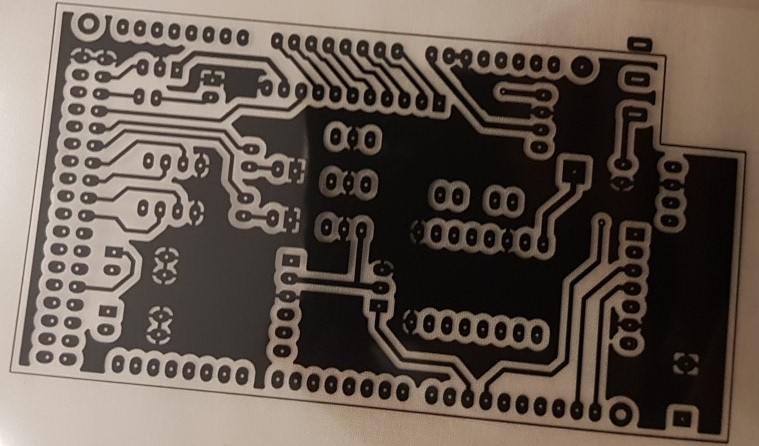
\includegraphics[width=.49\textwidth, height= \photoHeight]{figures/photolith_board1_top.jpg}}
	\subfigure[First example bottom layer]{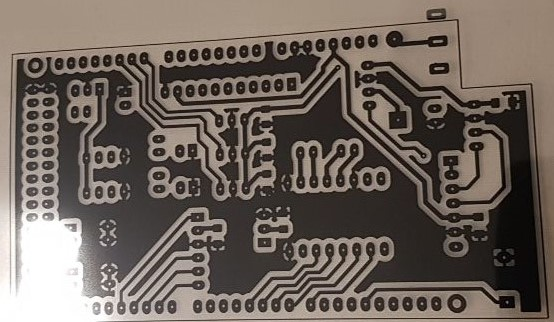
\includegraphics[width=.49\textwidth, height= \photoHeight]{figures/photolith_board1_bottom.jpg}}
	\subfigure[Second example top layer]{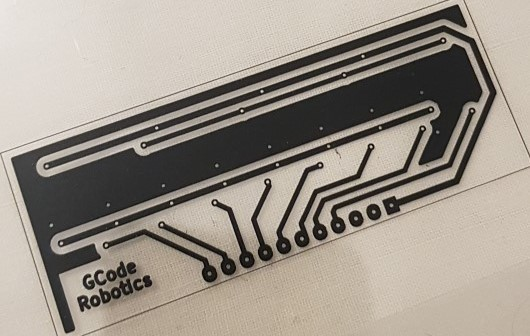
\includegraphics[width=.49\textwidth, height=\secondPhotoHeight]{figures/photolith_board2_top.jpg}}
	\subfigure[Second example bottom layer]{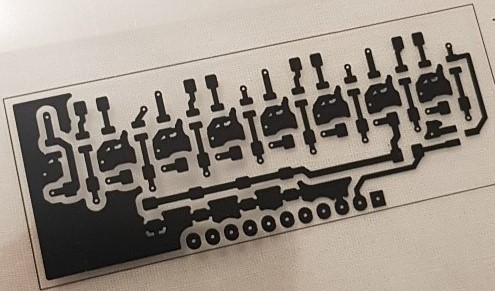
\includegraphics[width=.49\textwidth, height=\secondPhotoHeight]{figures/photolith_board2_bottom.jpg}}
	\caption{Two examples of double side PCBs photoliths}
	\label{fig:photo}
\end{figure}
%
%
\section{Copper plate insolation}\label{section:insol}
At this section, will be explained how to insolate the copper plate\footnote{Remember that the copper plate has to be photosensitive.} with the photoliths. First, if the copper plate is bigger than the desired printing size, it is necessary to use a shear machine to cut the copper plate and obtain the desired size. In the \autoref{fig:shear} it is shown the big copper plate placed in the shear machine, ready to be cut.
%
\begin{figure}[H]
	\centering
	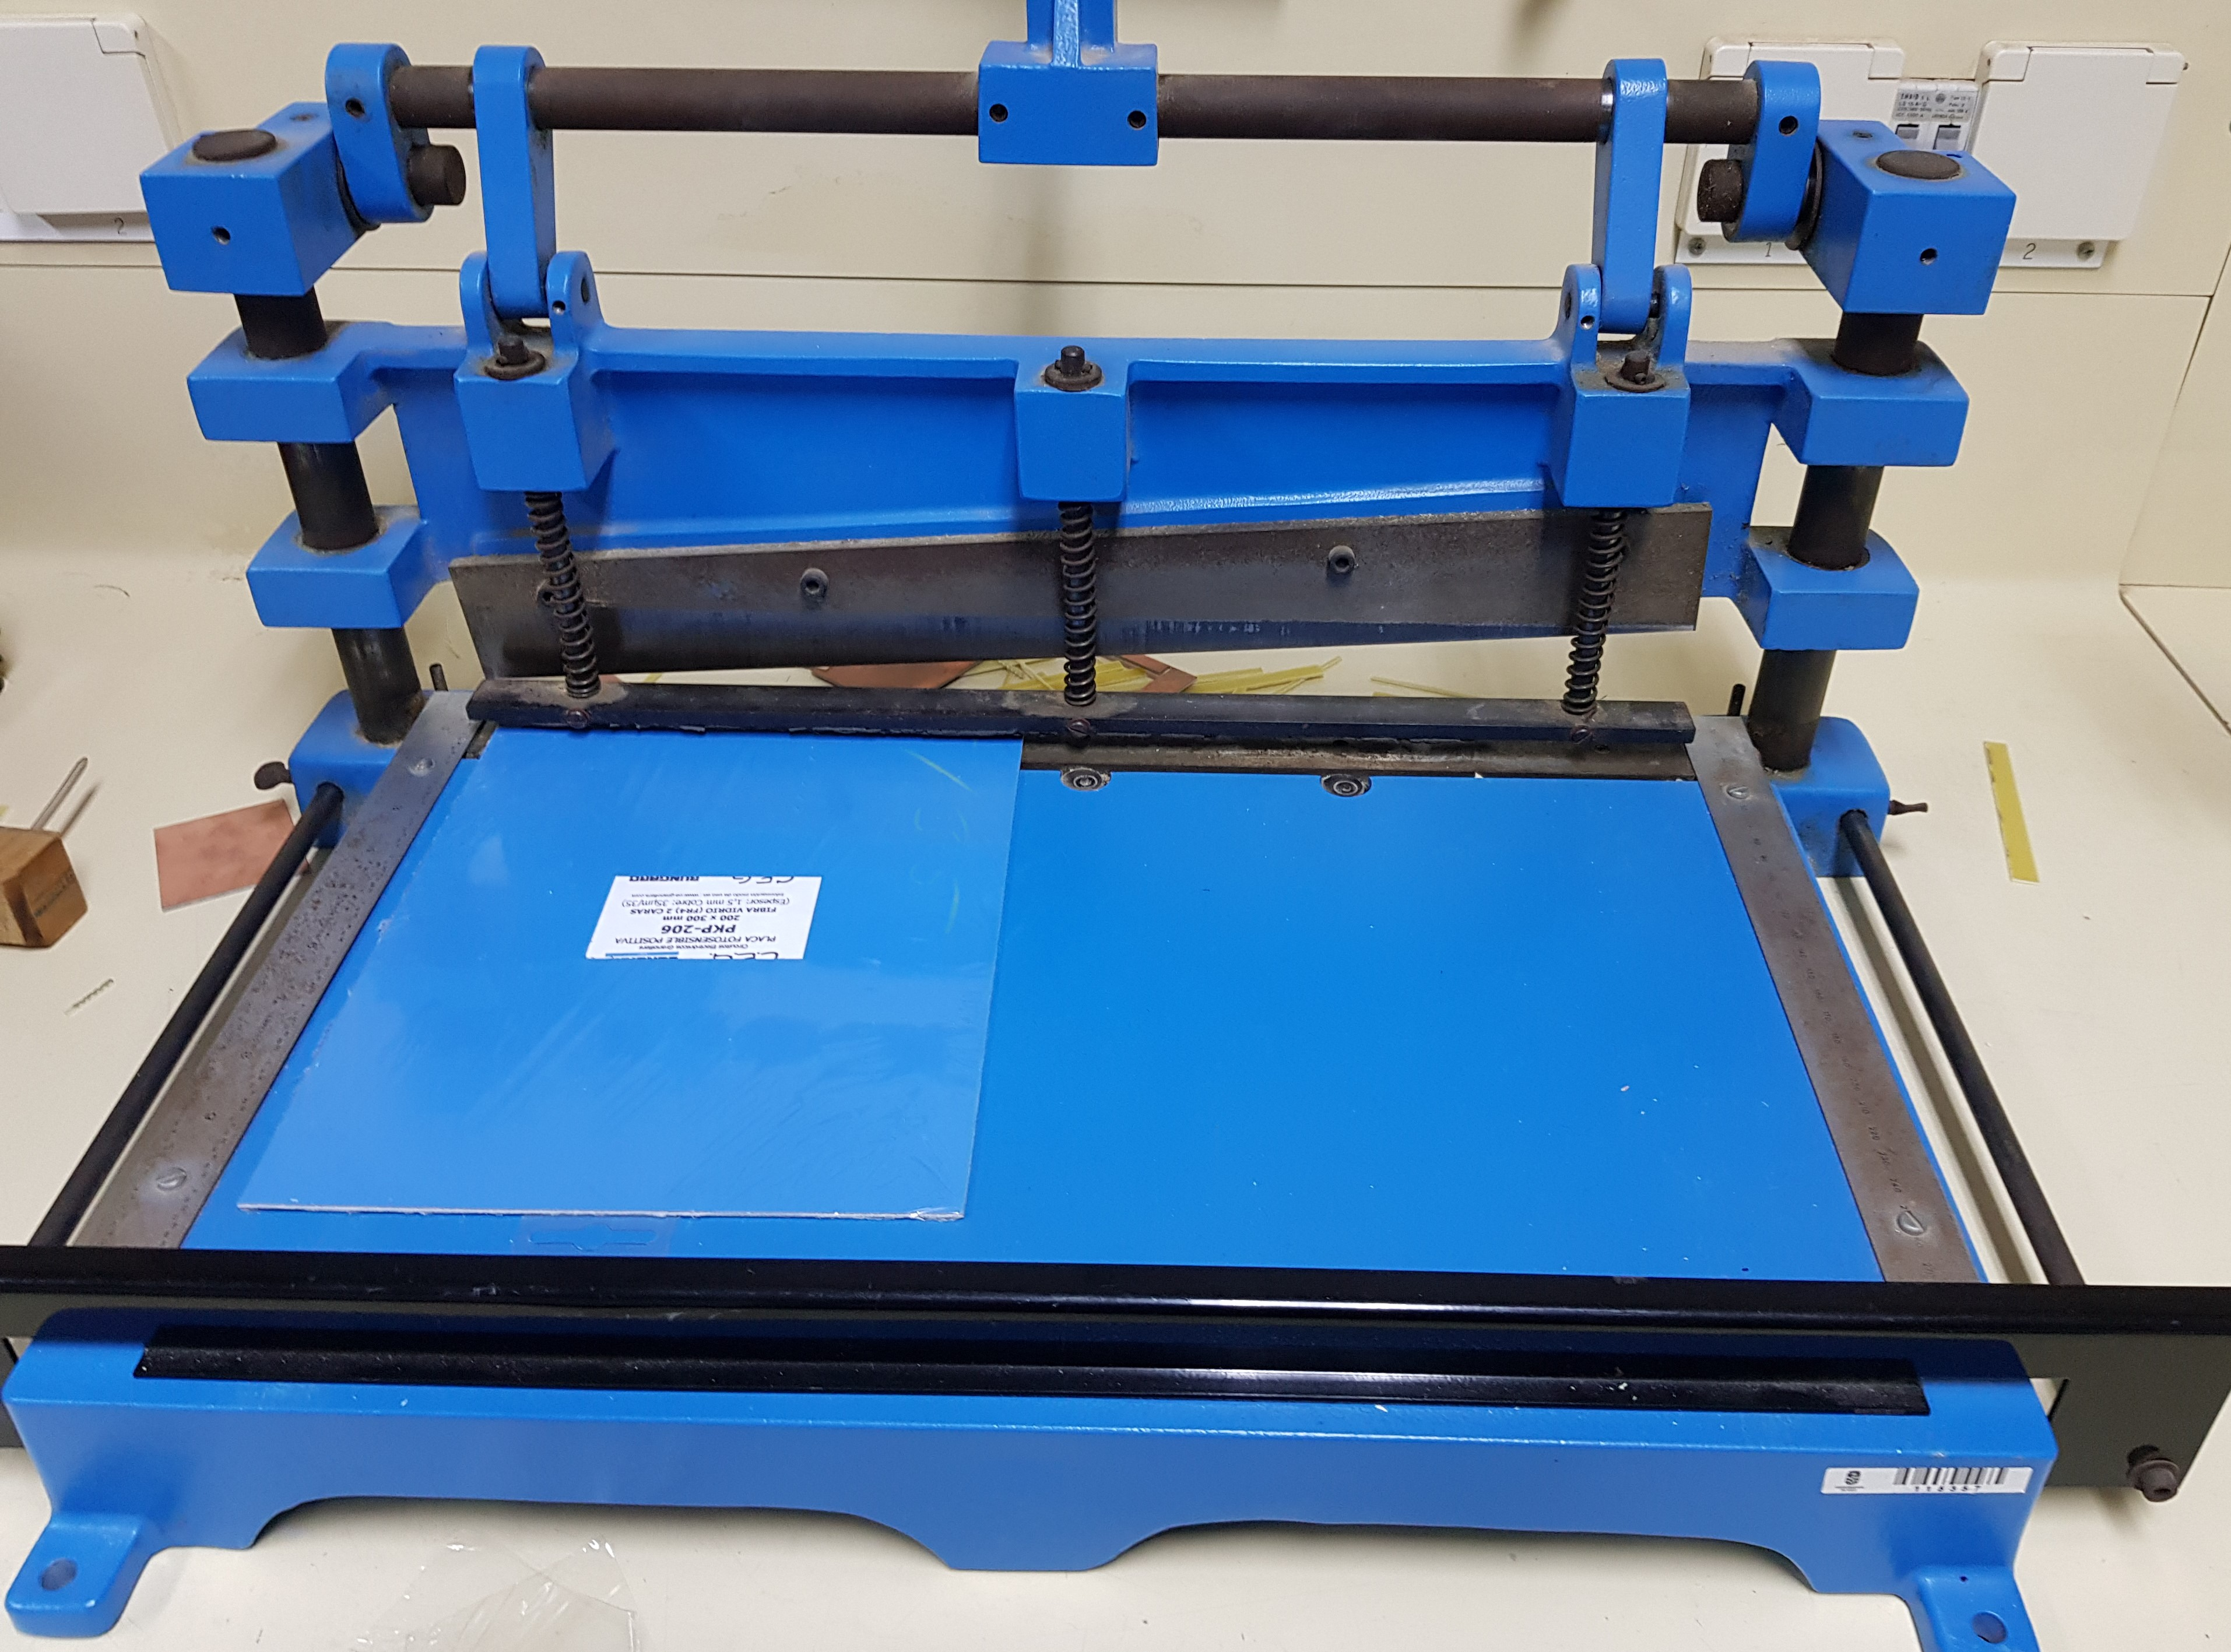
\includegraphics[width=.49\textwidth]{figures/process_cutting_shear.jpg}
	\caption{Shear machine with the cooper plate prepared}
	\label{fig:shear}
\end{figure}
%
After obtaining the copper plate with the desired size, it has to be inserted between the two photolith pairs and place it in the insolation machine like in the \autoref{fig:insol}. Make sure copper plate is correctly placed with the photoliths and centred in the insolation zone, in the second subfigure of the \autoref{fig:insol} it is zoomed in the collocation of the copper plate with the photoliths in the insolation zone.
%
\begin{figure}[H]
	\centering
	\subfigure[Global vision of the insolation machine]{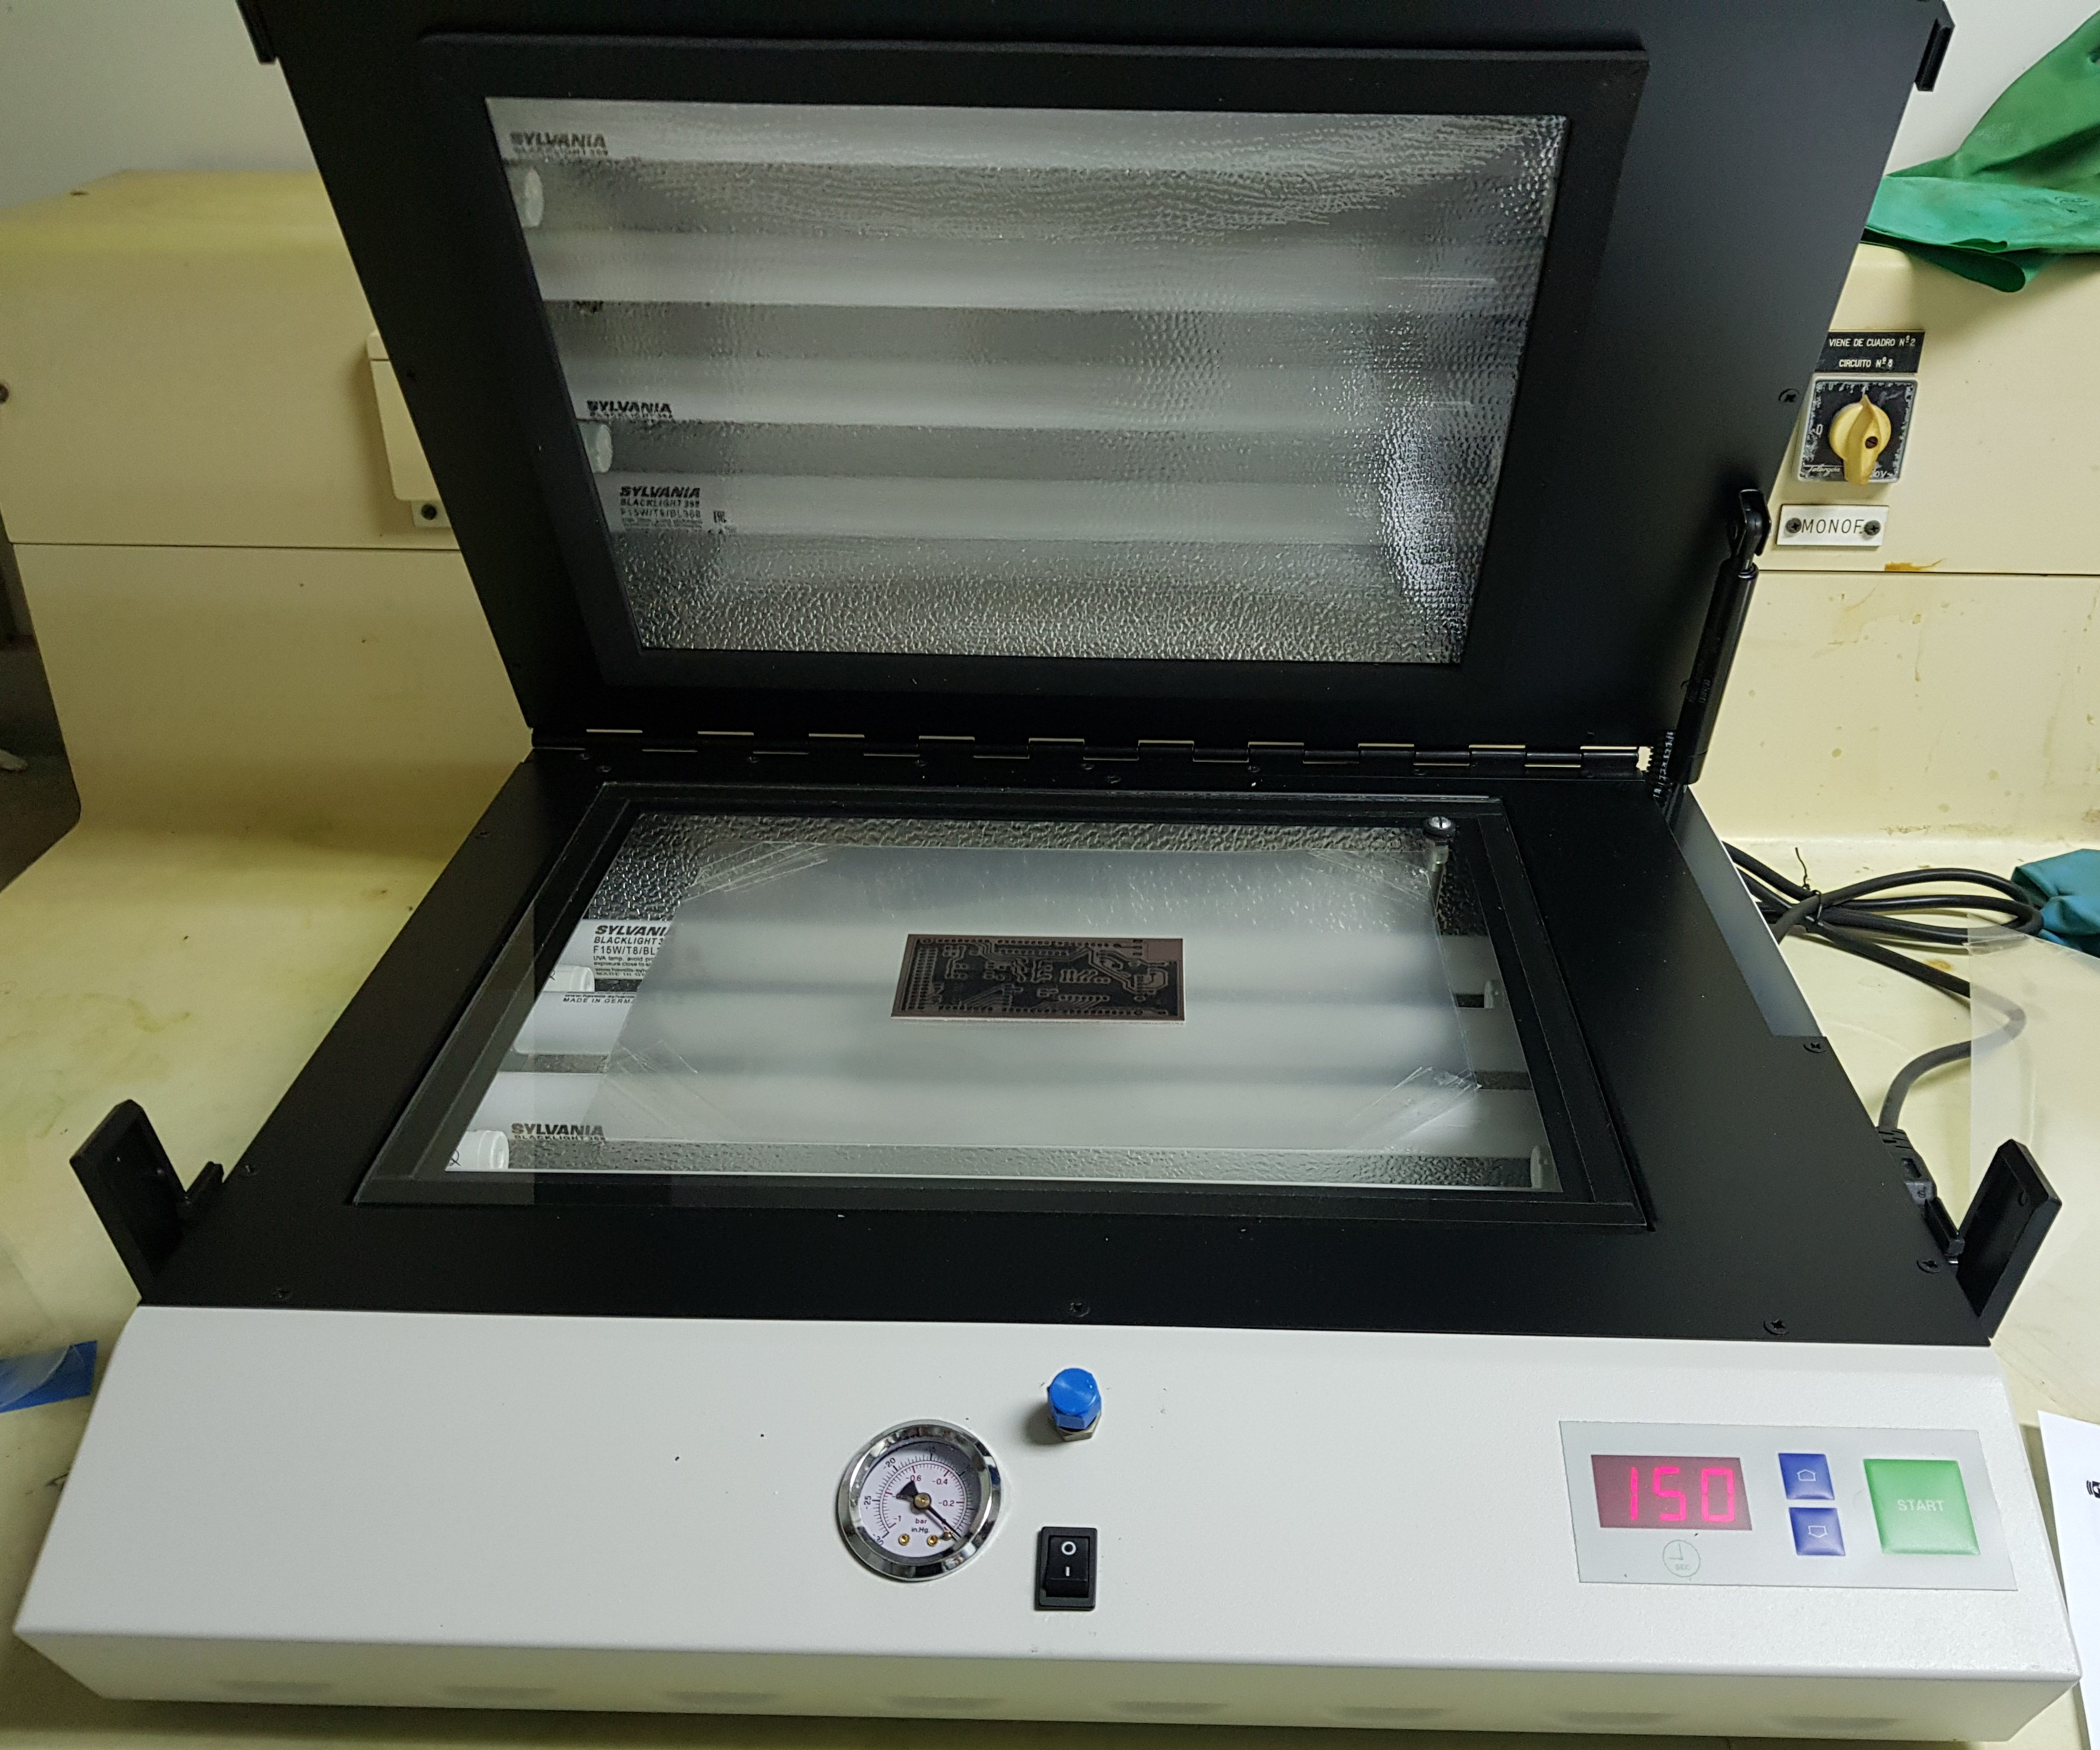
\includegraphics[width=.49\textwidth, height=\insolHeight]{figures/process_insolation_machine_open.jpg}}
	\subfigure[Zoom in on the PCB with the photolites]{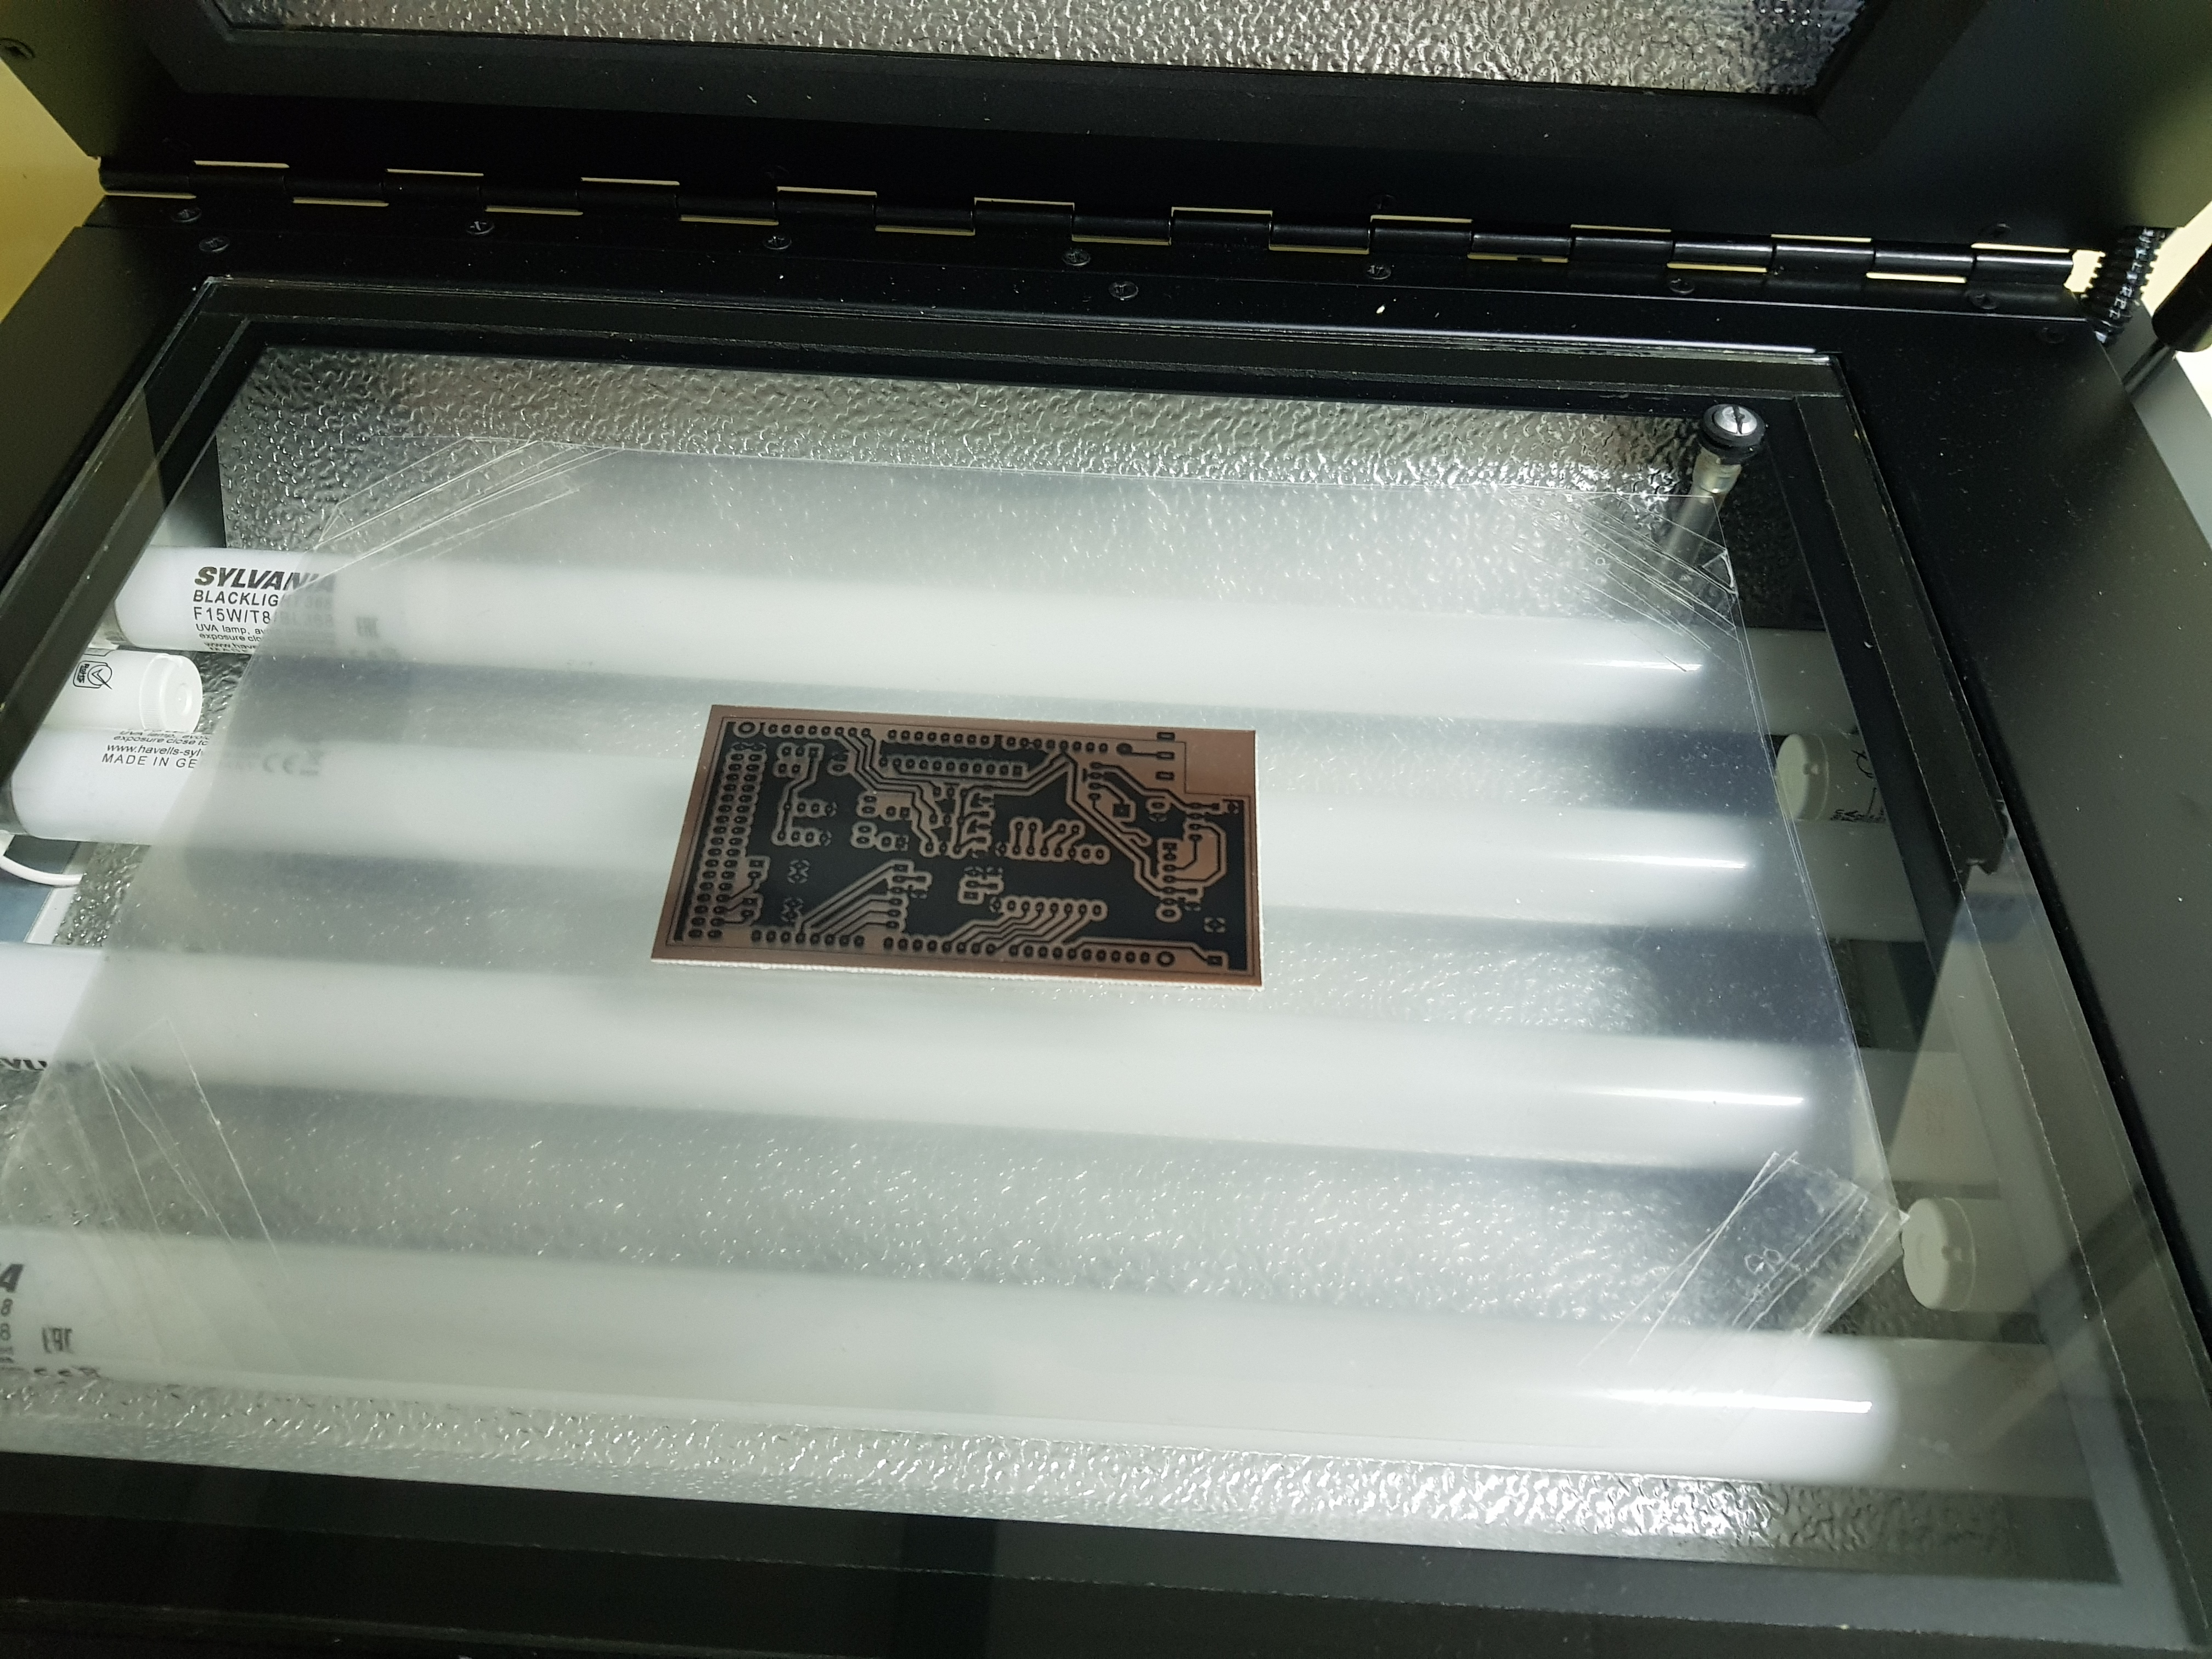
\includegraphics[width=.49\textwidth, height=\insolHeight]{figures/process_insolation_pcb_placement.jpg}}
	\caption{Insolation machine with the PCB and the photoliths ready}
	\label{fig:insol}
\end{figure}
%
With all of this placed, the insolation machine has to be closed, locked, and turn on the black switch of the \autoref{fig:insolClosed}. This will empty the interior of the insolation machine, where the copper plate is placed. Now, use the blue buttons to set the insolation interval time that it is shown on the display. At this case, 150 seconds\footnote{It depends on the insolation machine and the age of the copper plate} is the time set. Press the green button ``START'' and the insolation process will start. This insolation time corrupts the protecting layer of the copper layer. During this time it is advisable to do the tasks of the \autoref{section:prep}.
%
\begin{figure}[H]
	\centering
	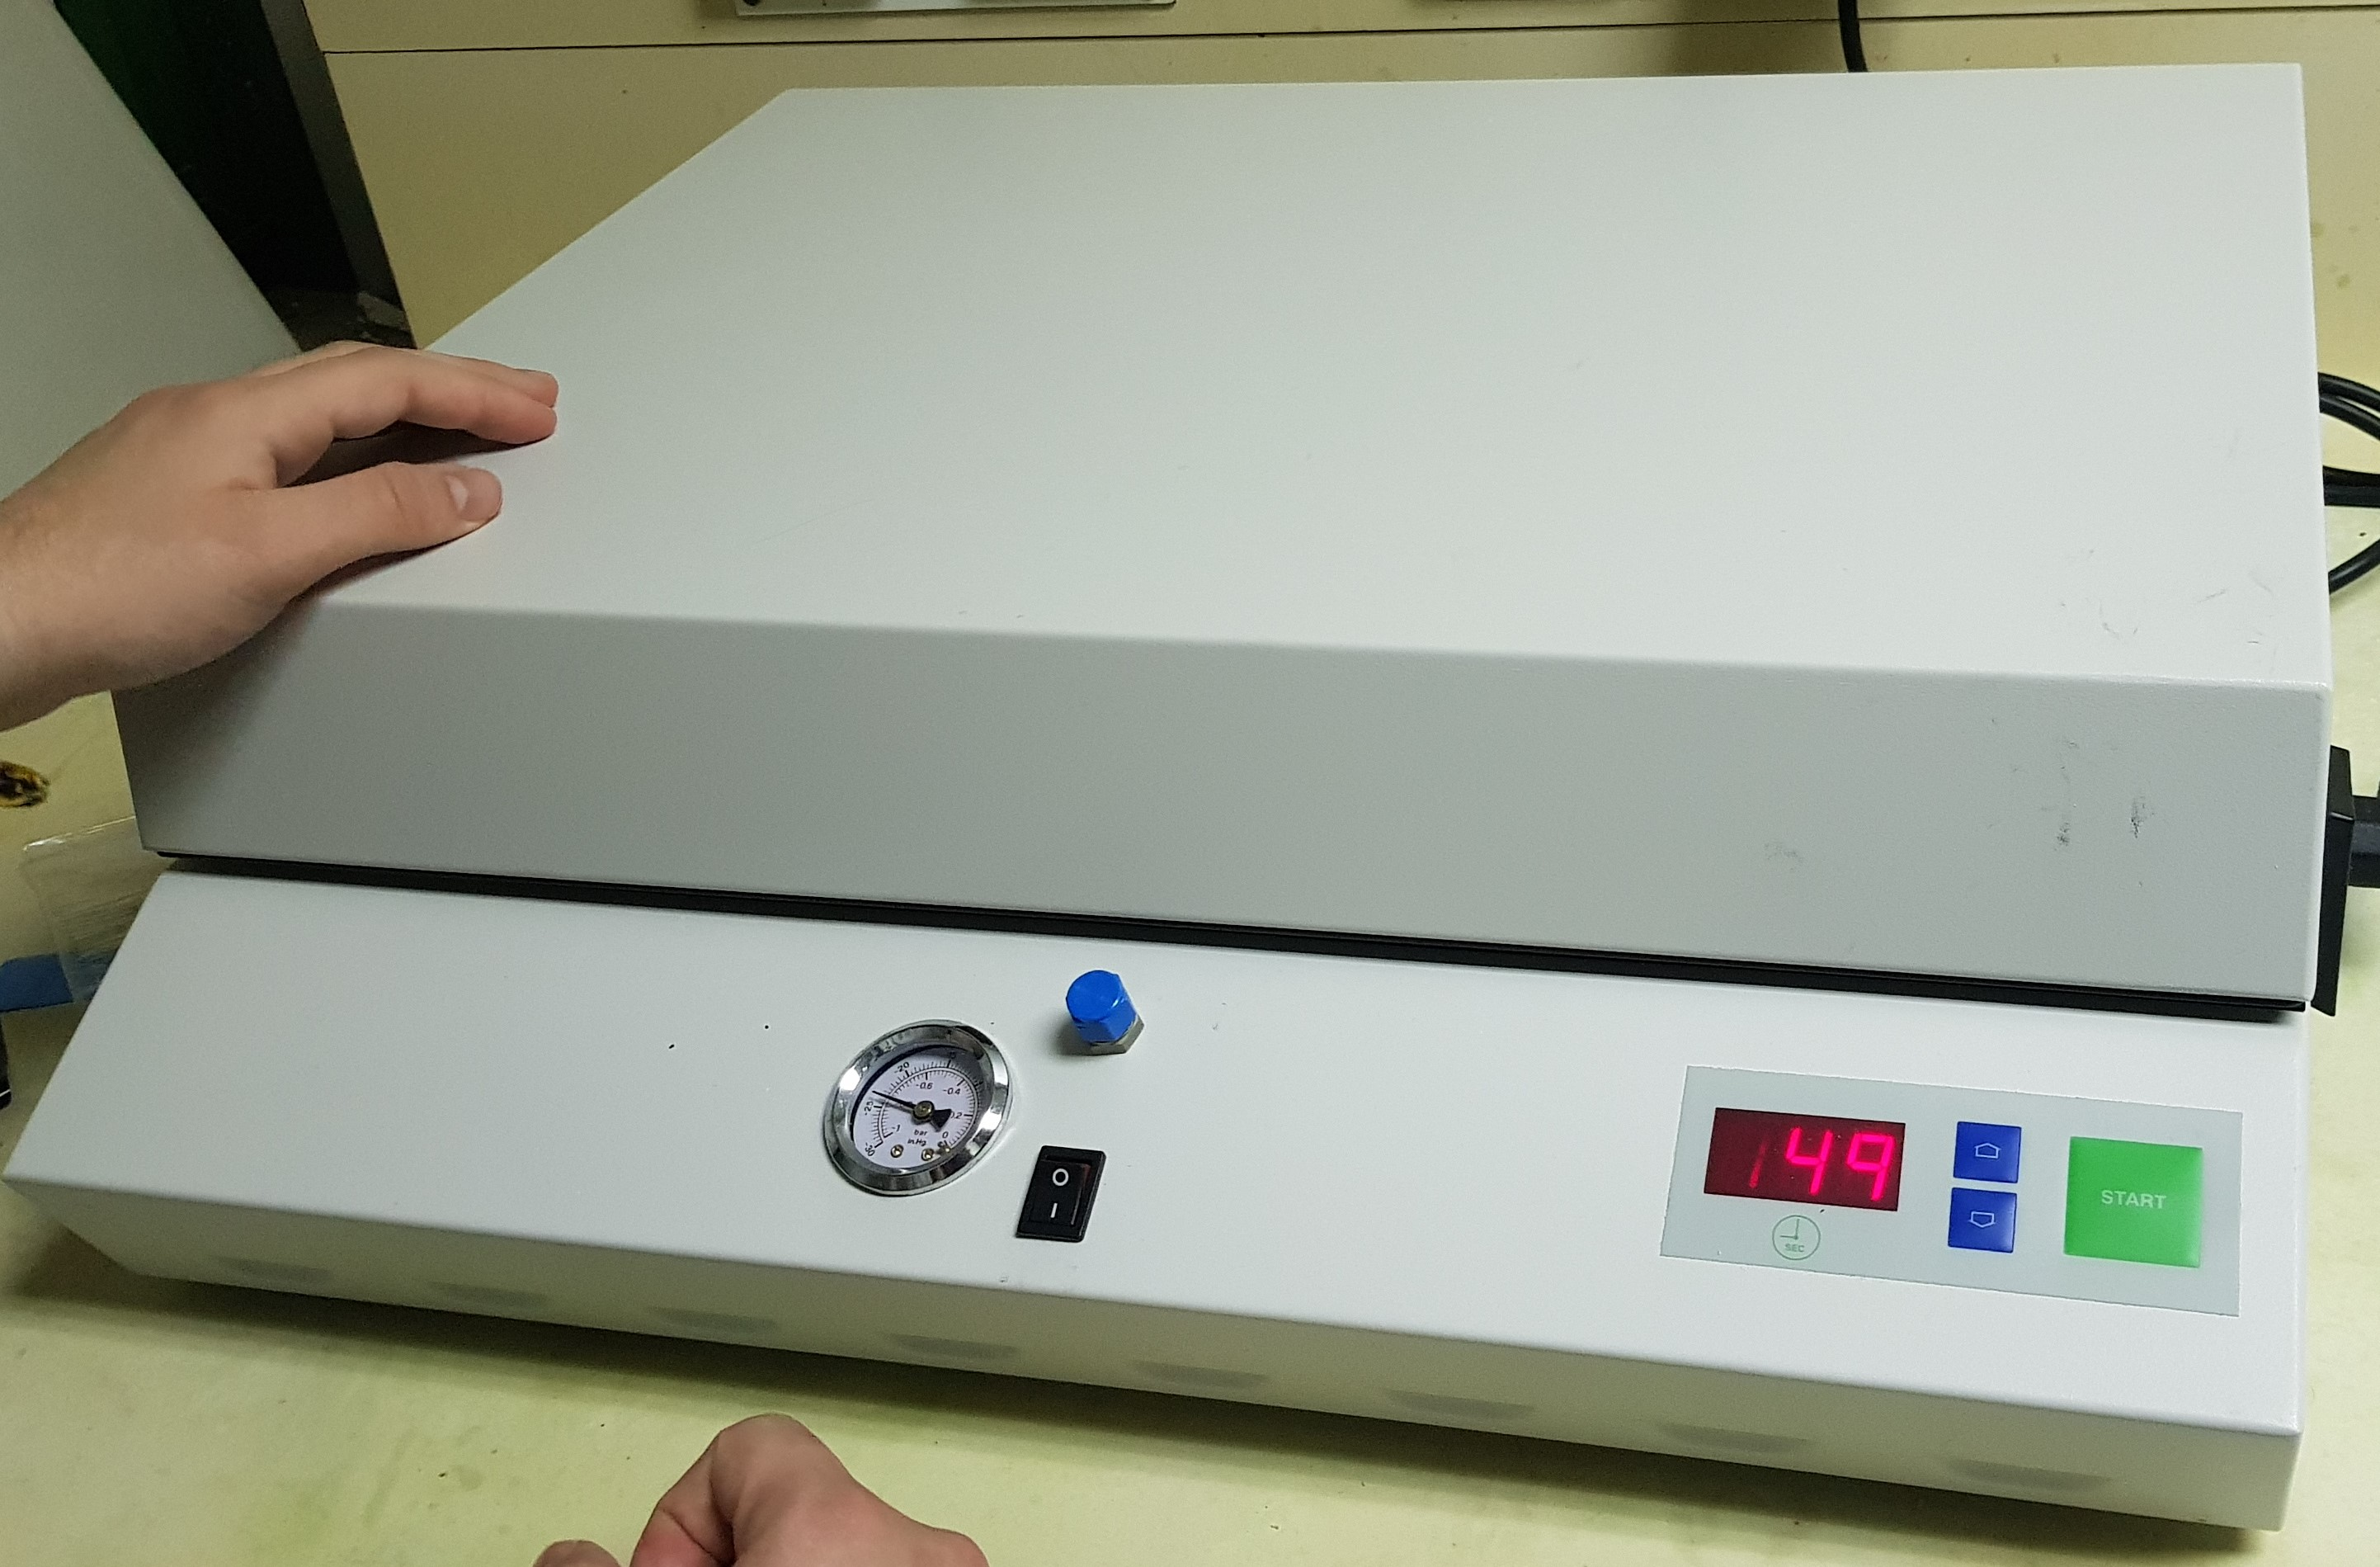
\includegraphics[width=.49\textwidth]{figures/process_insolation_machine_closed.jpg}
	\caption{Insolation machine during the insolation process}
	\label{fig:insolClosed}
\end{figure}
%
When this process ends, turn off the empty of the machine interior, take the copper plate and you will be able to see a really small difference in the colour between the protected and unprotected zones of the copper layers. Now, it is the turn of the tasks of the \autoref{section:soda}.
%
\section{Preparation of the caustic soda and the acid mix}\label{section:prep}
During the insolation, it is a good idea to prepare the caustic soda and the acid mix. The material needed for the PCB cleaning is shown in the first subfigure of the \autoref{fig:prep}. 

For the caustic soda preparation it's only necessary a container and the caustic soda\footnote{What a surprise!}. The brown liquid shown in the second subfigure of the \autoref{fig:prep} is relative to this caustic soda because it has been reused several times.

In the case of the acid mix it is a bit more complex and it can not be reused. This transparent mix ``can'' be seen in the second subfigure of the \autoref{fig:prep} and it has the next admixtures with its ratio\footnote{Remember to wear gloves and use an air extractor and a security screen}:
\begin{itemize}
	\item Water $\Rightarrow$ 15\%
	\item Hydrogen peroxide $\Rightarrow$ 30\%
	\item Hydrochloric acid at 36\% $\Rightarrow$ 15\%
\end{itemize}
%
\begin{figure}[H]
	\centering
	\subfigure[Material needed for the PCB cleaning]{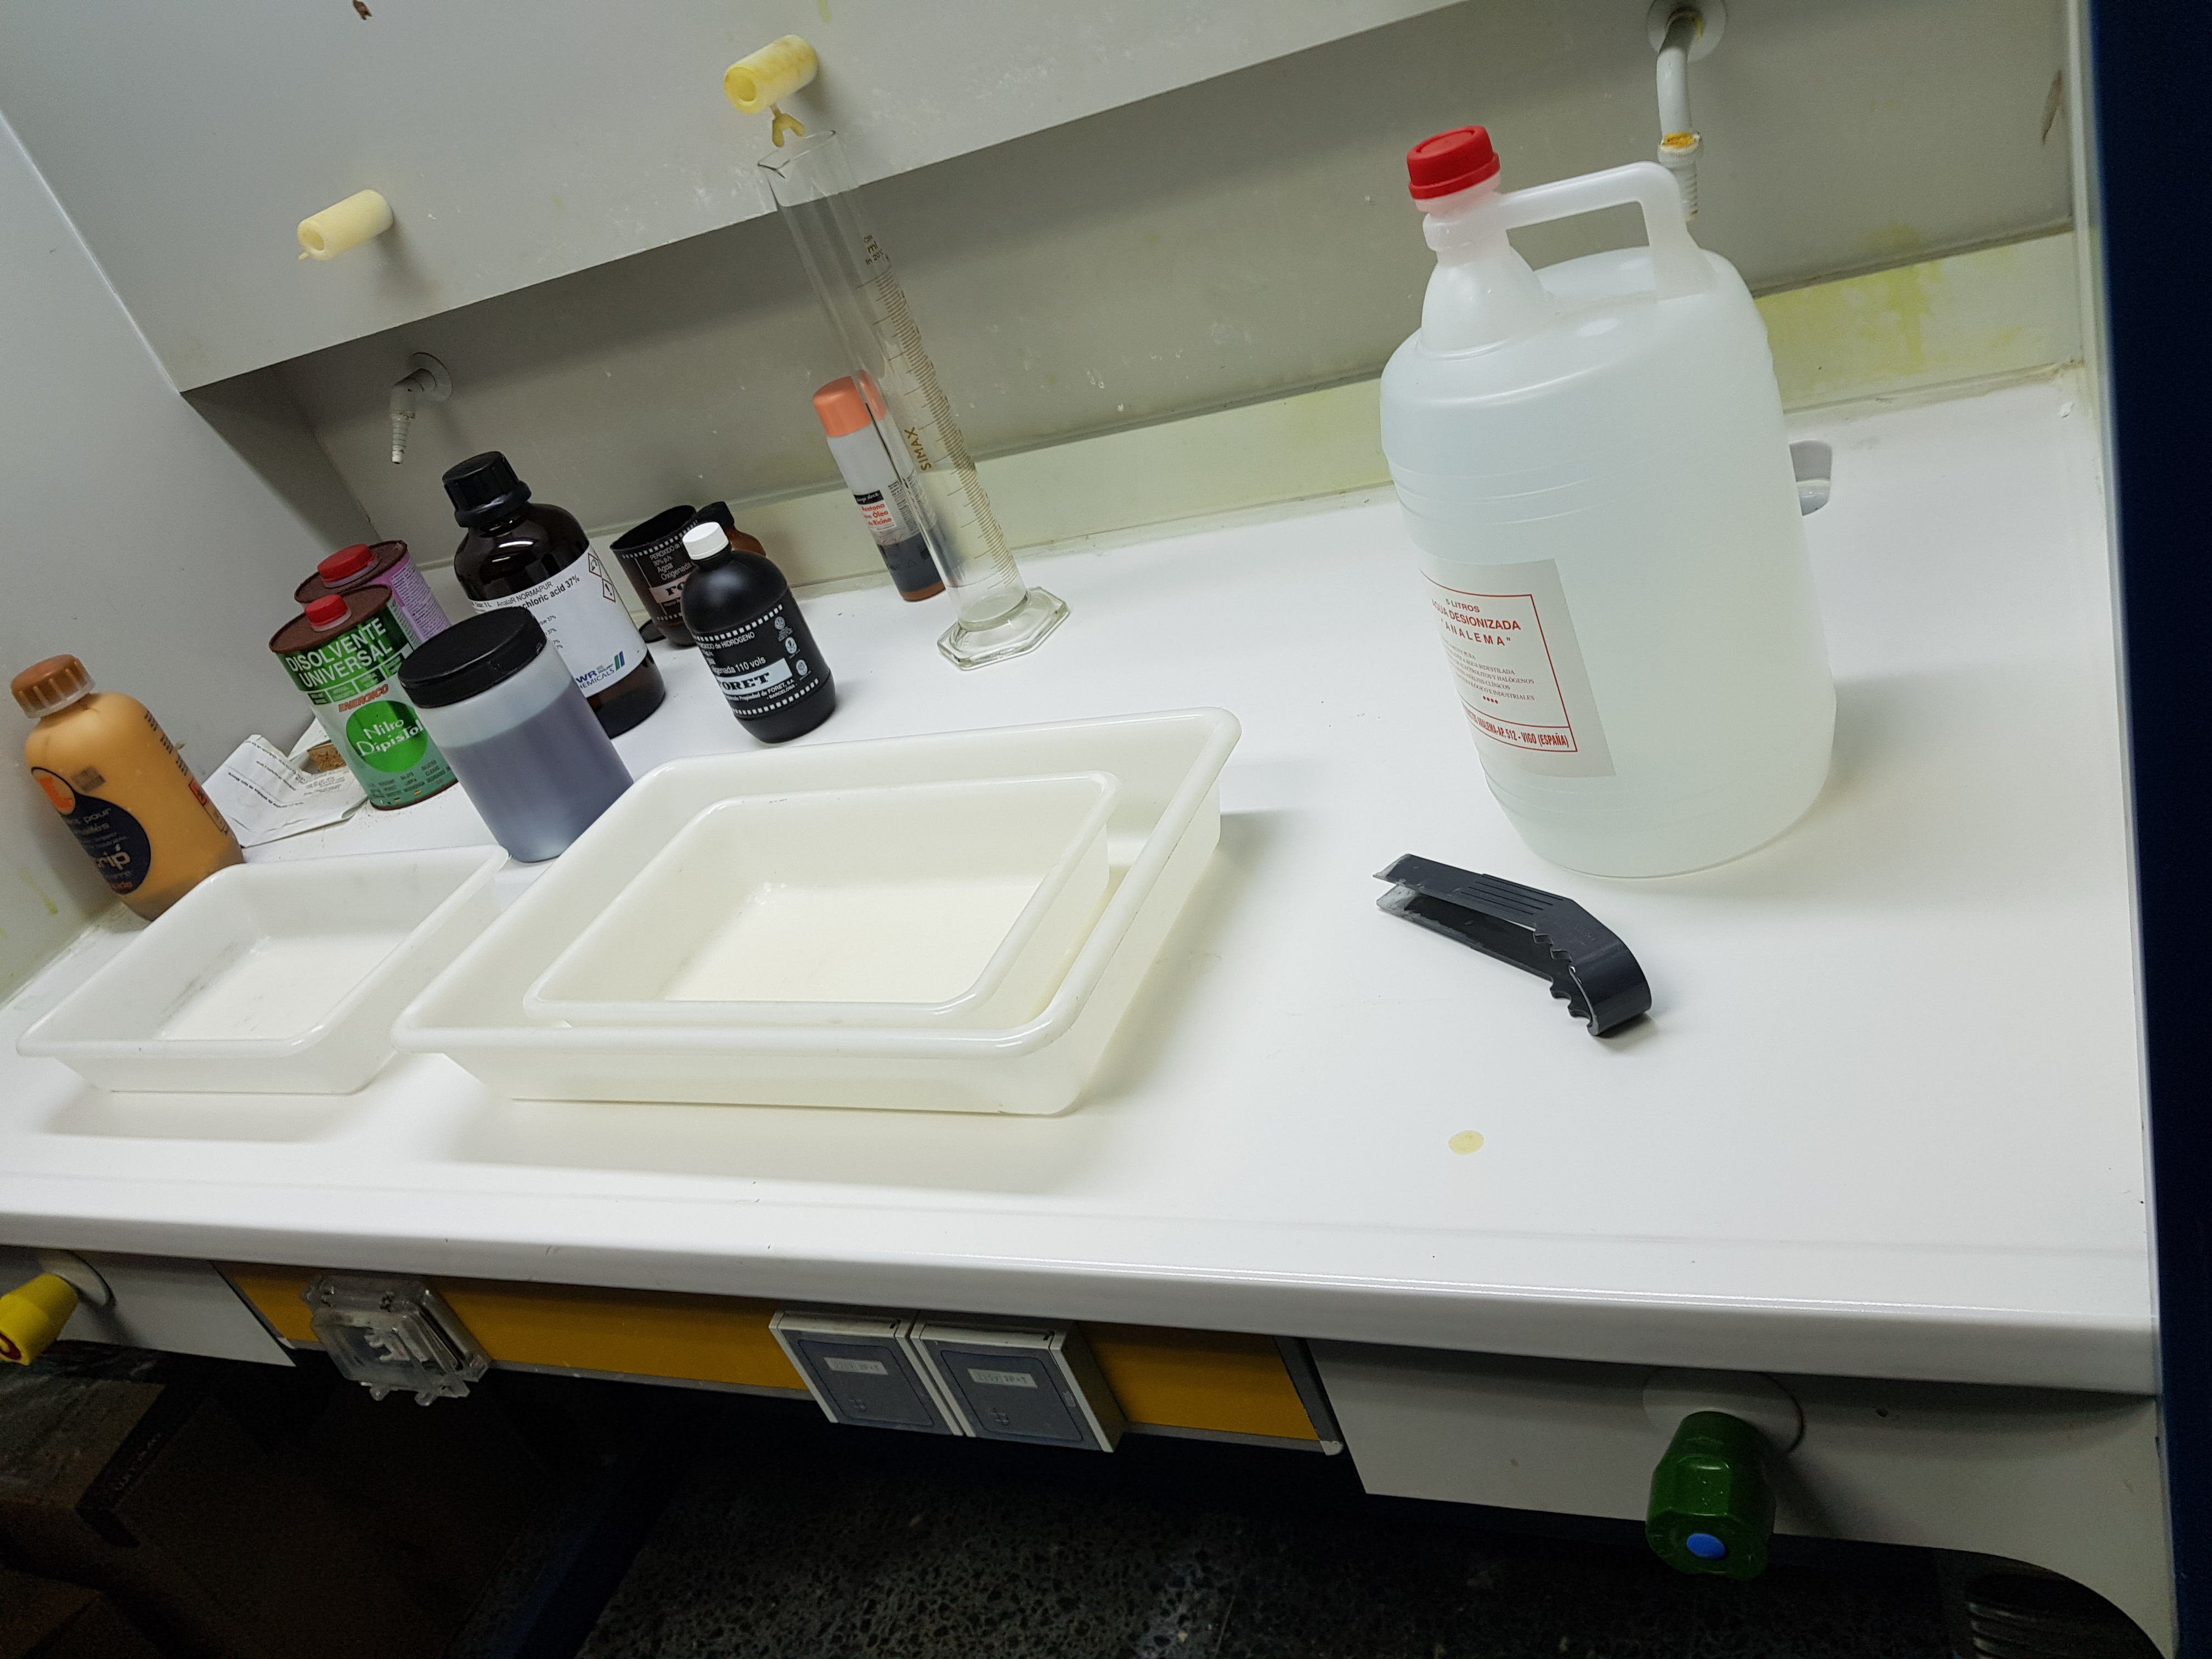
\includegraphics[width=.49\textwidth]{figures/process_chemicals_materials.jpg}}
	\subfigure[soda and acid containers prepared]{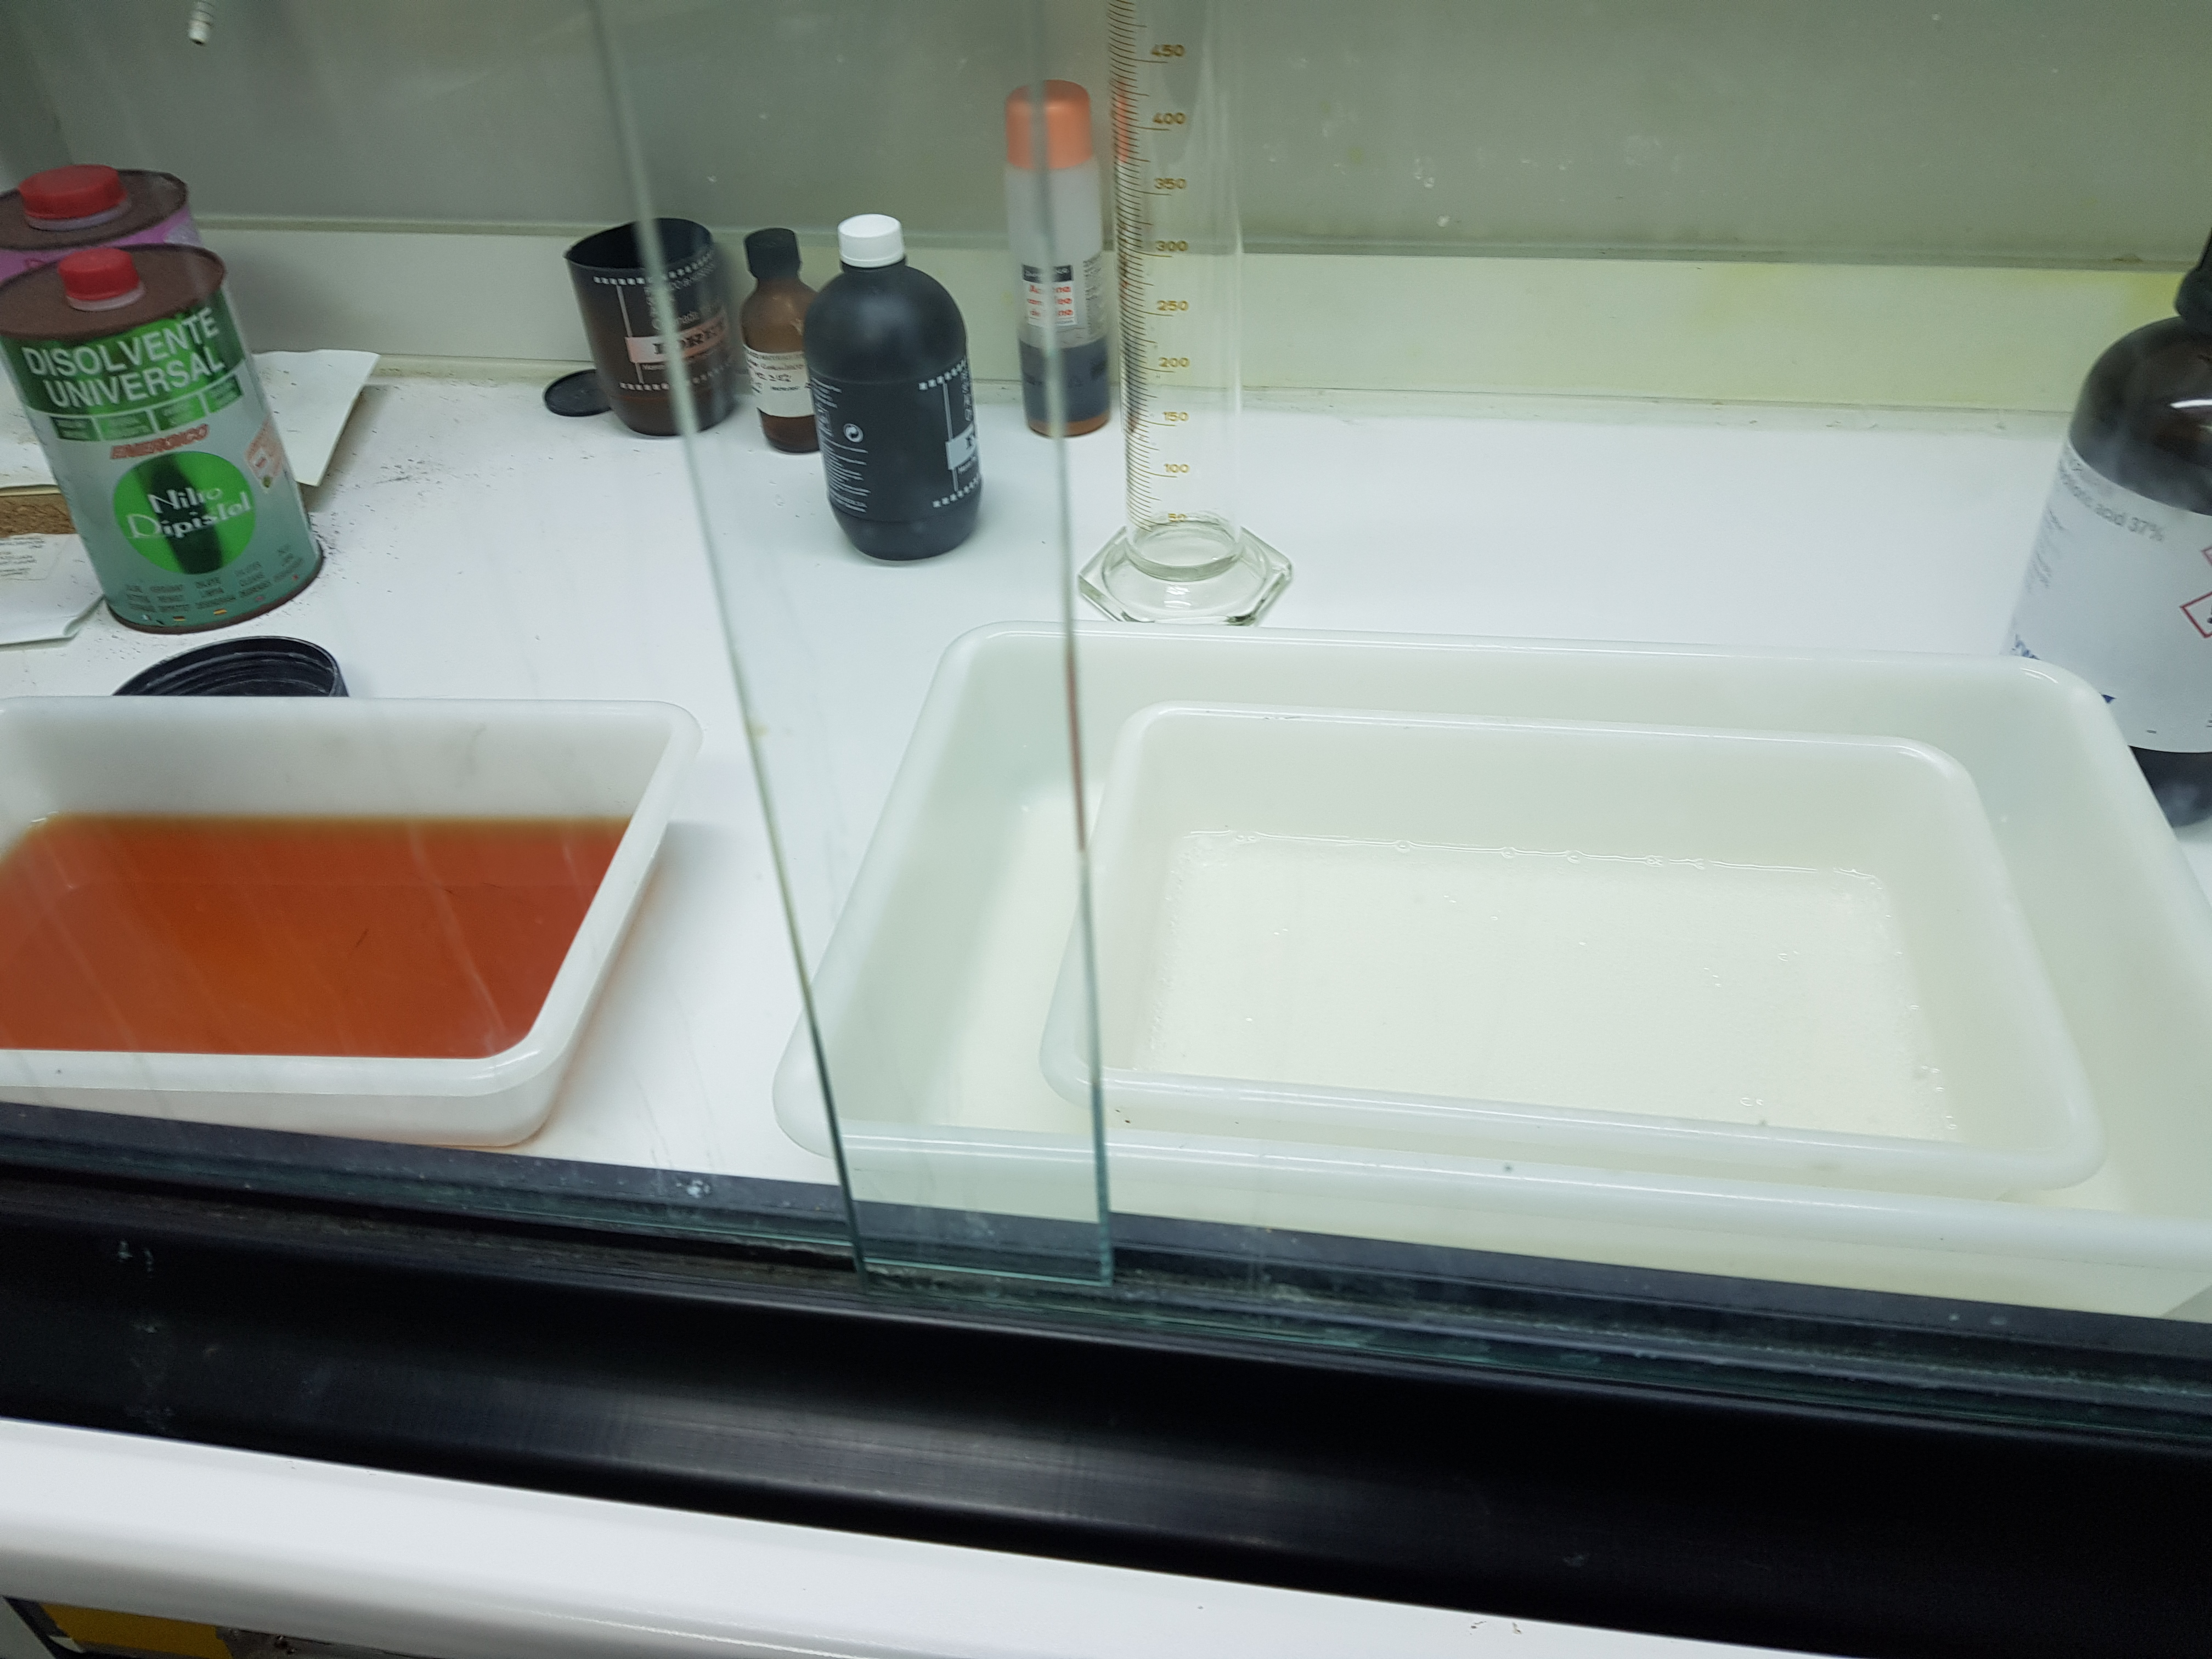
\includegraphics[width=.49\textwidth]{figures/process_chemicals_containers.jpg}}
	\caption{Setup of the soda and acid containers for the PCB cleaning}
	\label{fig:prep}
\end{figure}
%
\section{Caustic soda cleaning}\label{section:soda}
Coming from the \autoref{section:insol} now the copper plate has to be introduced in the container prepared with caustic soda and we have to move it slowly in the soda with soft tweezers, being careful about scratching the copper layers.
%
\begin{figure}[H]
	\centering
	\subfigure[Global vision of the insolation machine]{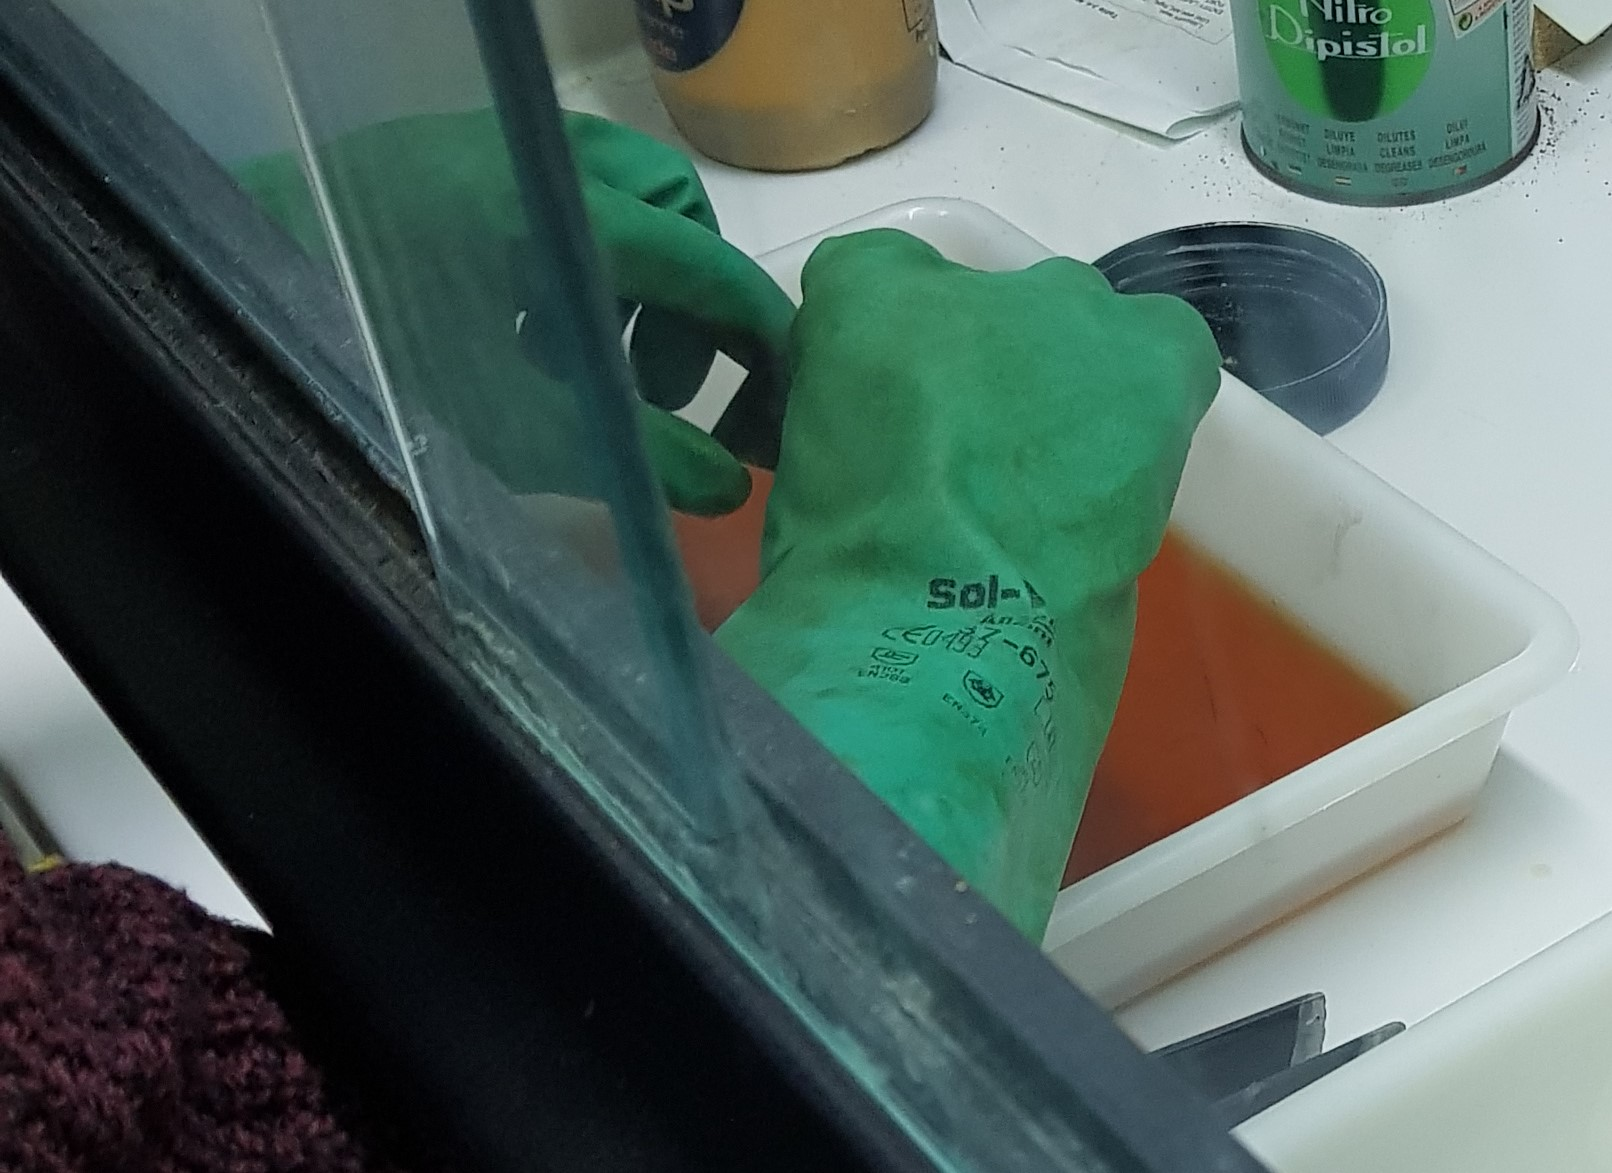
\includegraphics[width=.49\textwidth, height=\insolHeight]{figures/process_soda_immersion.jpg}}
	\subfigure[Zoom in the PCB with the photolites]{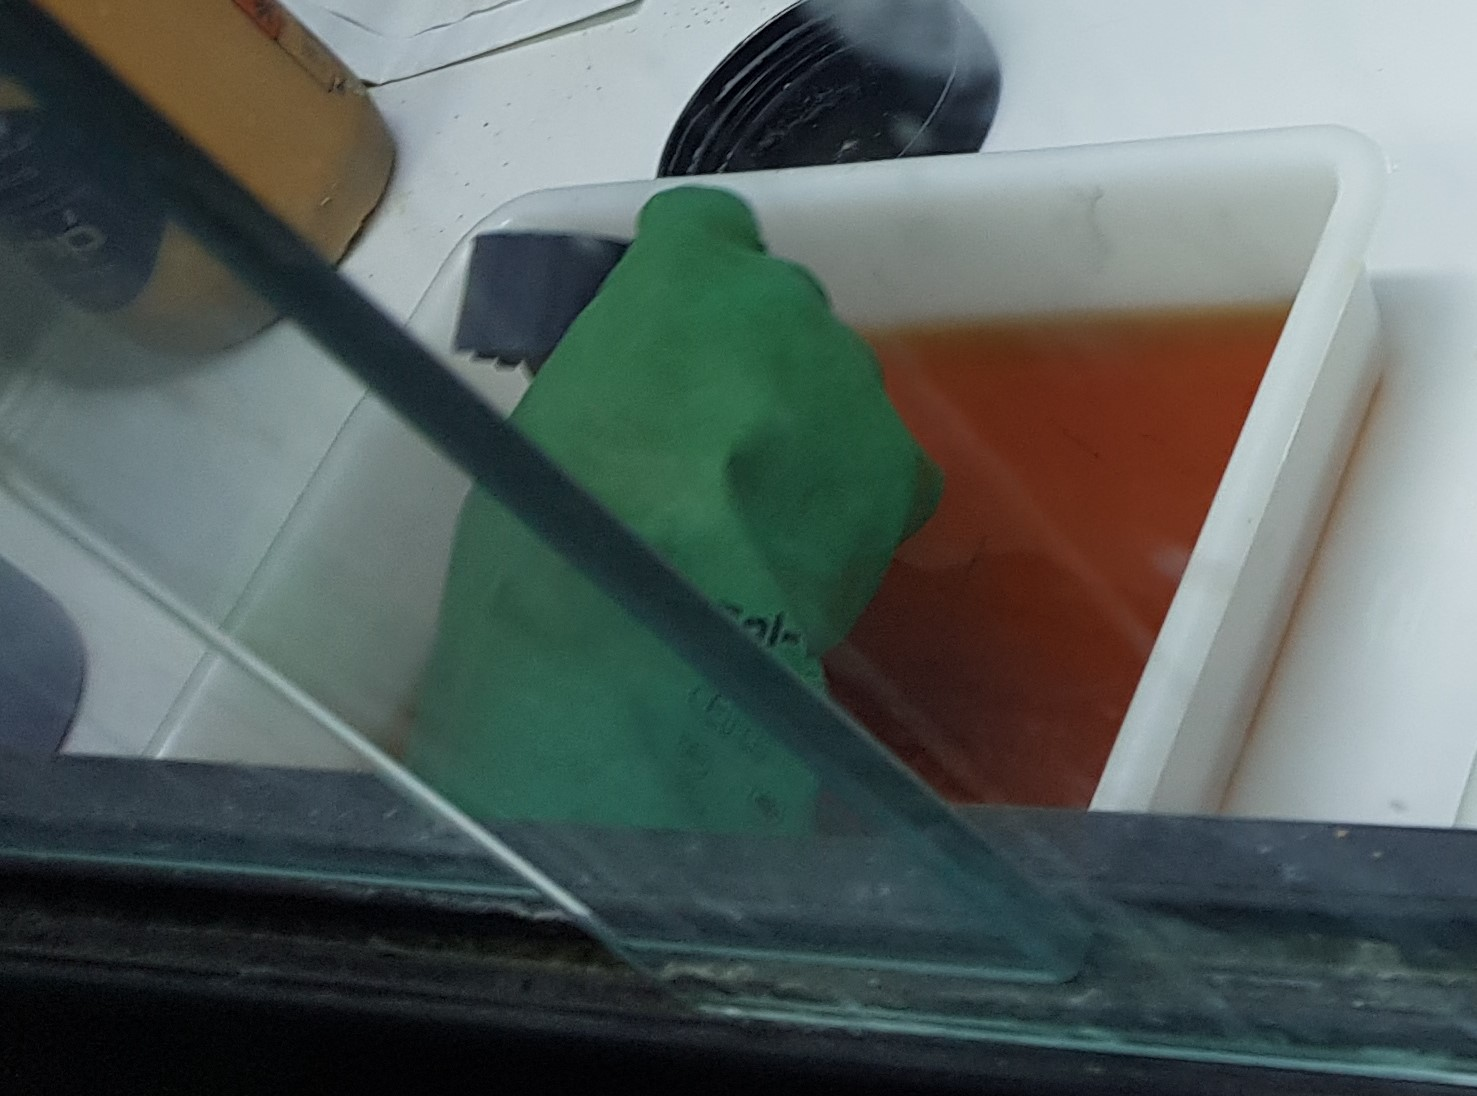
\includegraphics[width=.49\textwidth, height=\insolHeight]{figures/process_soda_detail.jpg}}
	\caption{Insolation machine with the PCB and the photolites ready}
	\label{fig:soda}
\end{figure}
%
The copper plate will be ready for taking it out of the caustic soda when its appearance seems like the copper plate shown in the \autoref{fig:aftersoda}, all the footprints and traces have to be well defined. The dark zones keep the copper protector and the other zones no longer have this protector.

Now, both layers have to be cleaned with water and paper to delete the caustic soda that remains on the surface of both layers. It needs to be dried with paper after this.
%
\begin{figure}[H]
	\centering
	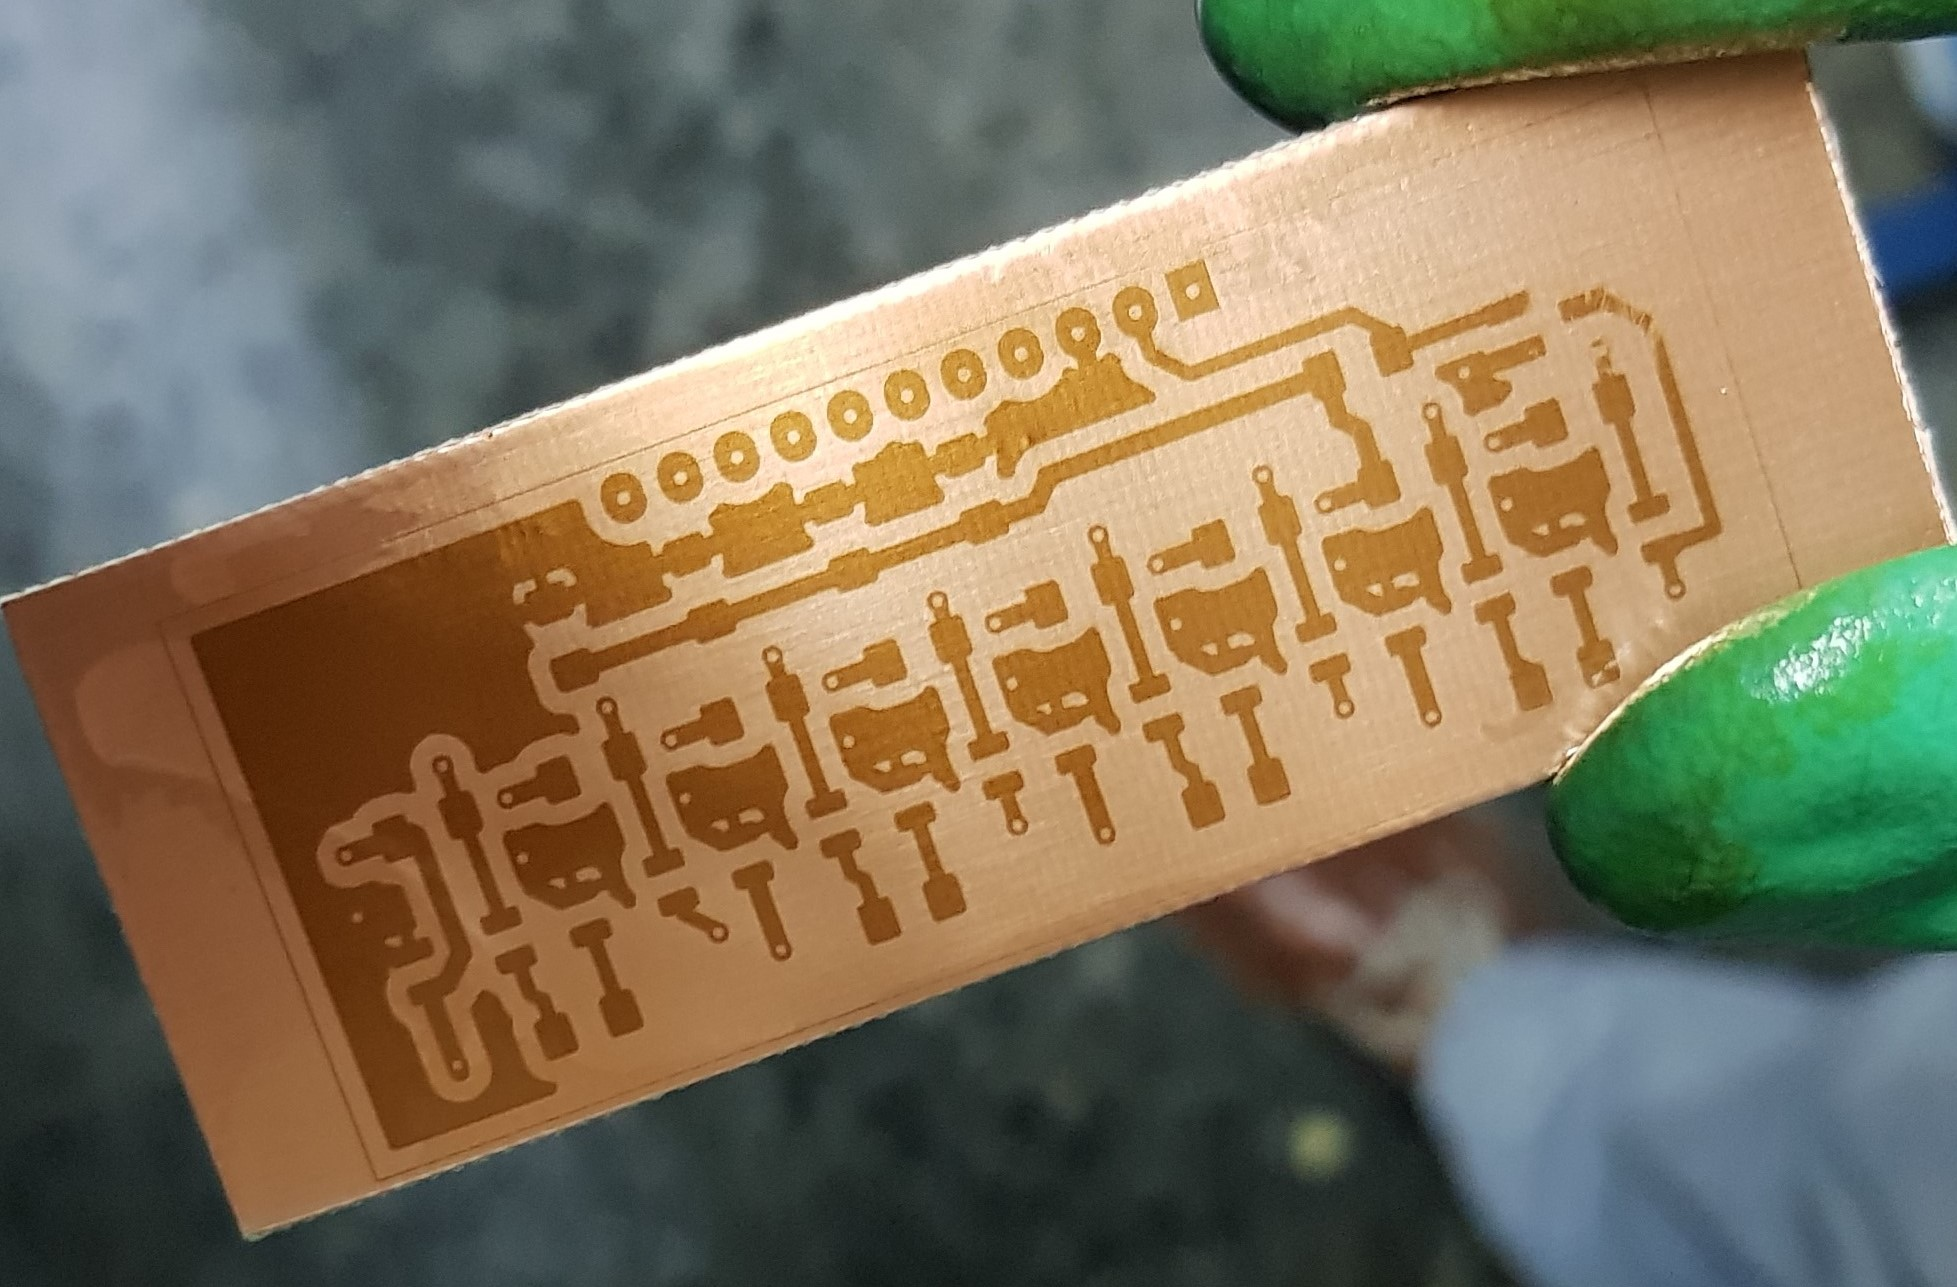
\includegraphics[width=.7\textwidth]{figures/pcb_result_after_soda.jpg}
	\caption{PCB view after soda cleaning}
	\label{fig:aftersoda}
\end{figure}
%
%
\section{Acid cleaning}\label{section:acid}
The process with the acid mix is similar to caustic soda cleaning. Introduce the copper plate in the container with the acid mix and move it using tweezers or tilting the container\footnote{Be careful with the acid mix!} as shown in the \autoref{fig:acid}. 
%
\begin{figure}[H]
	\centering
	\subfigure[Start of the copper cleaning with acid]{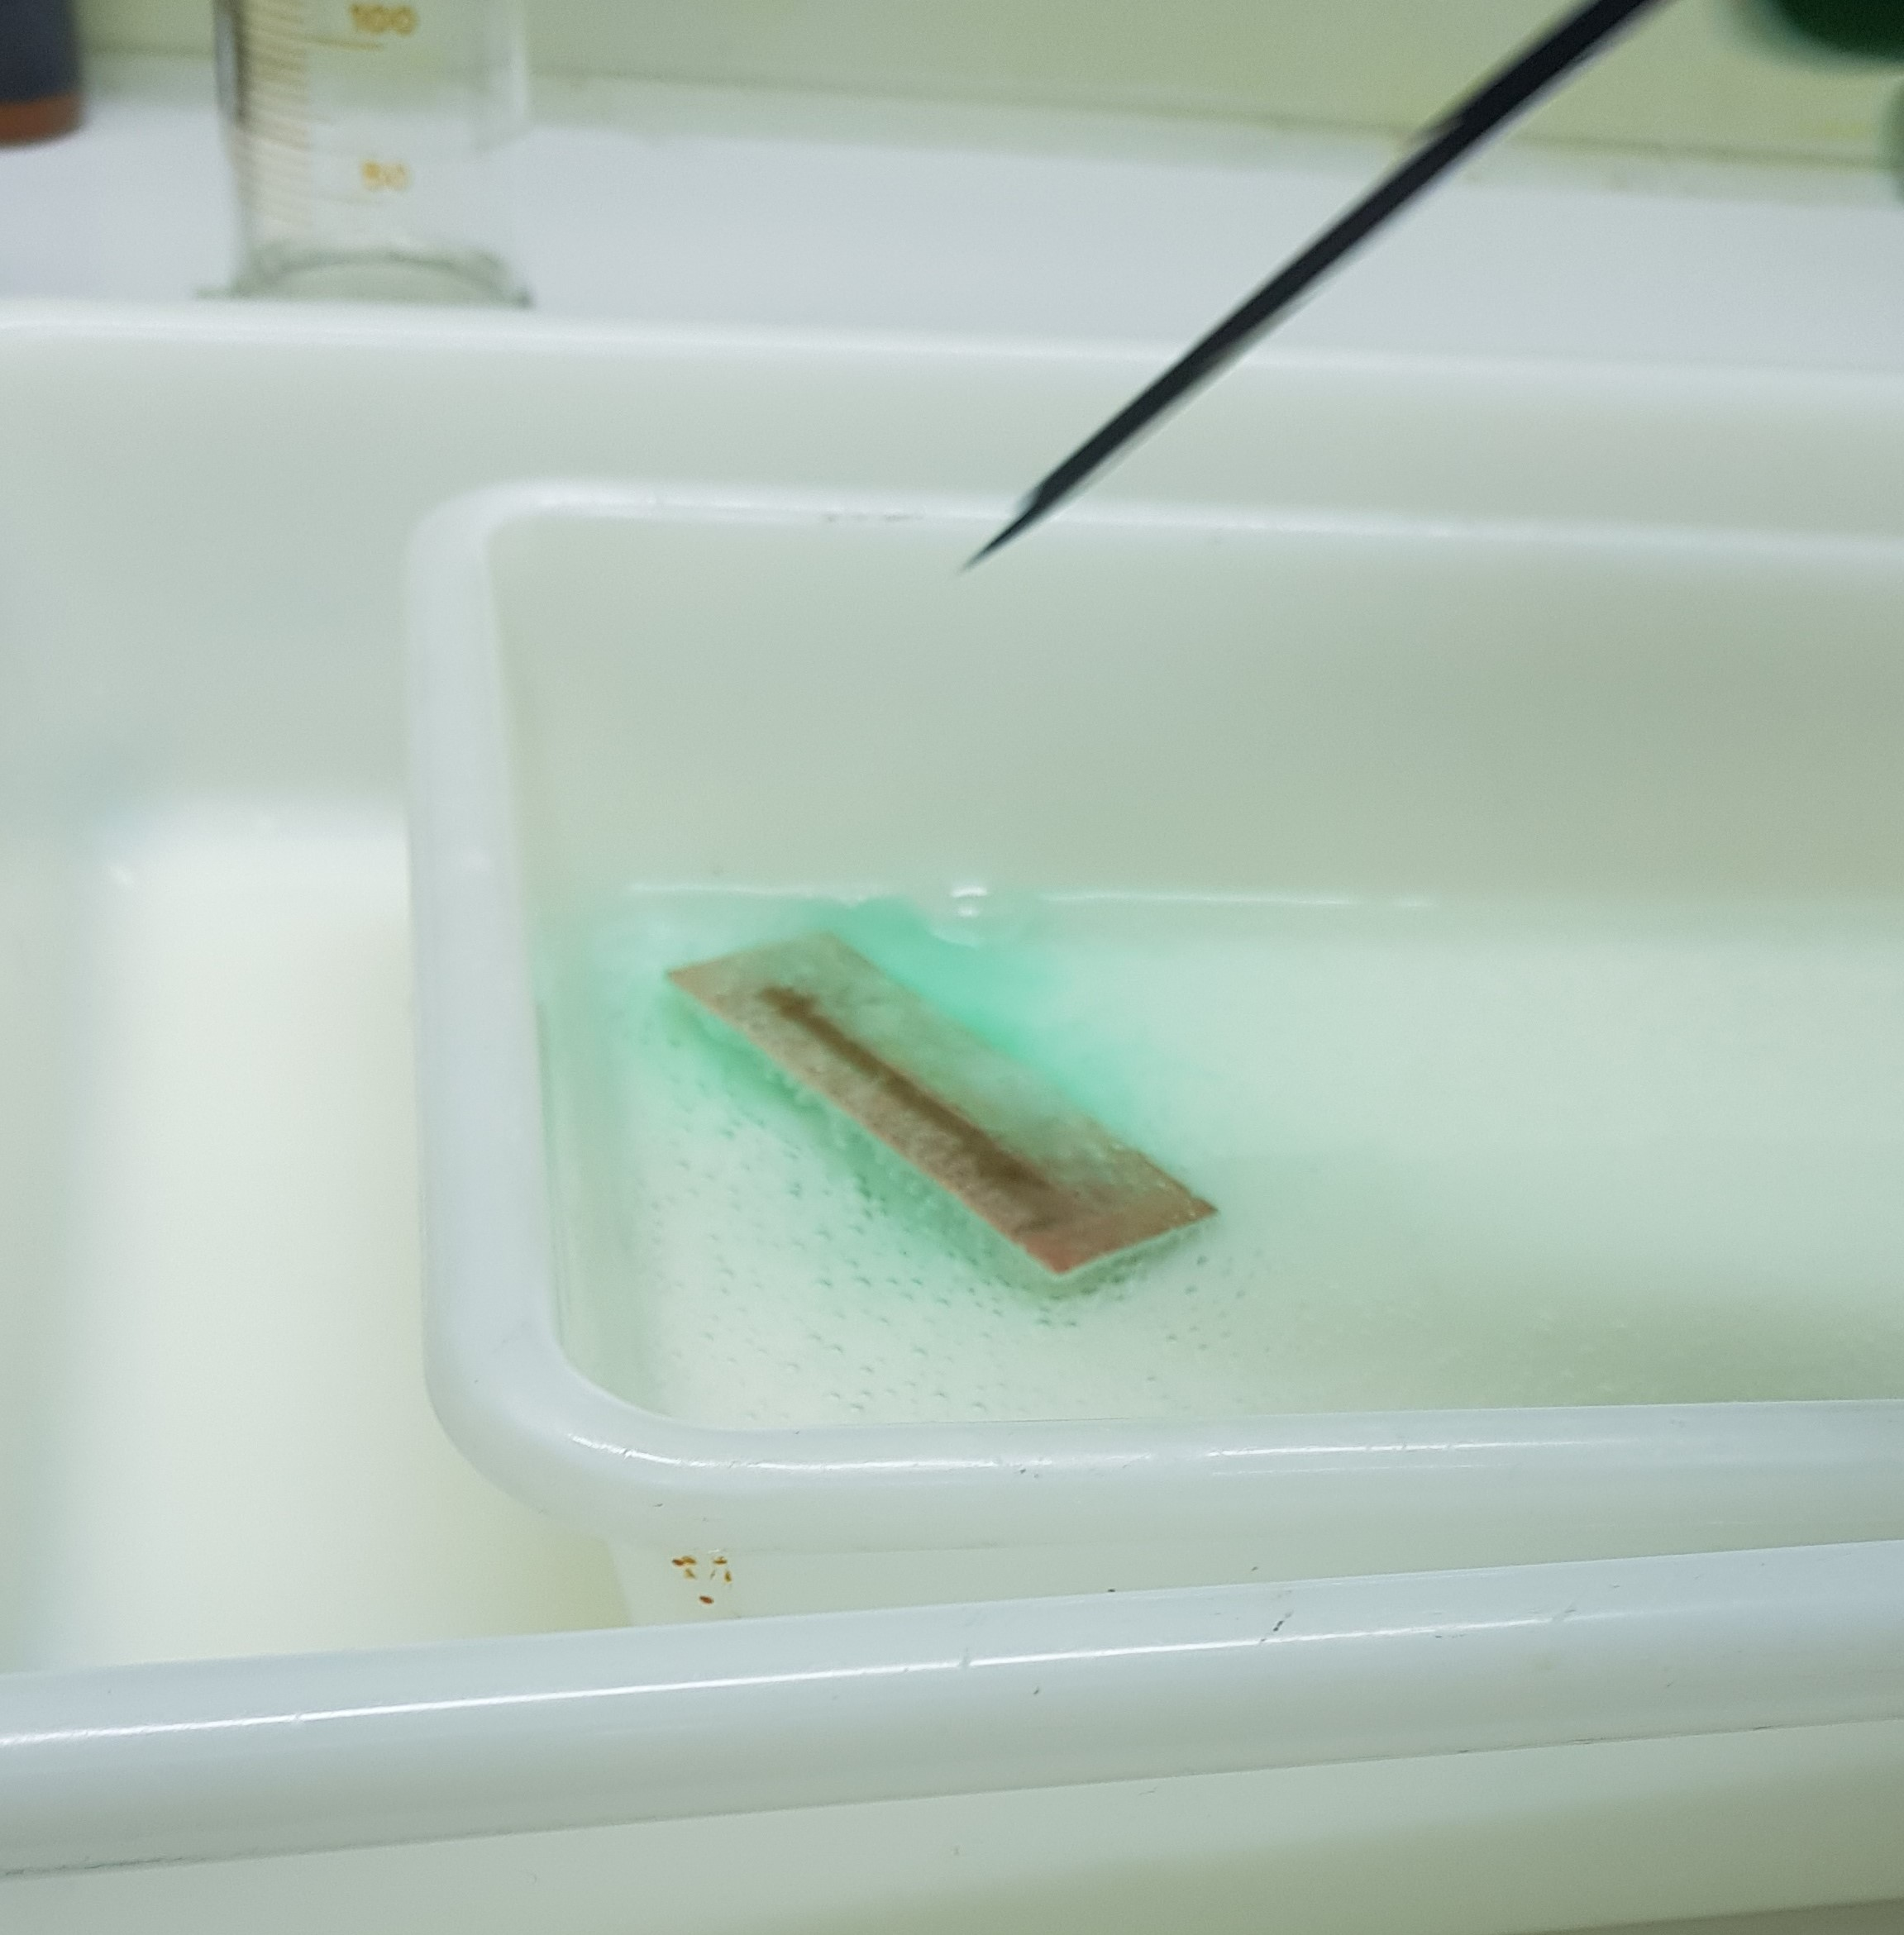
\includegraphics[width=.49\textwidth, height=\acidHeight]{figures/process_etching_start.jpg}}
	\subfigure[Moving the PCB in the acid]{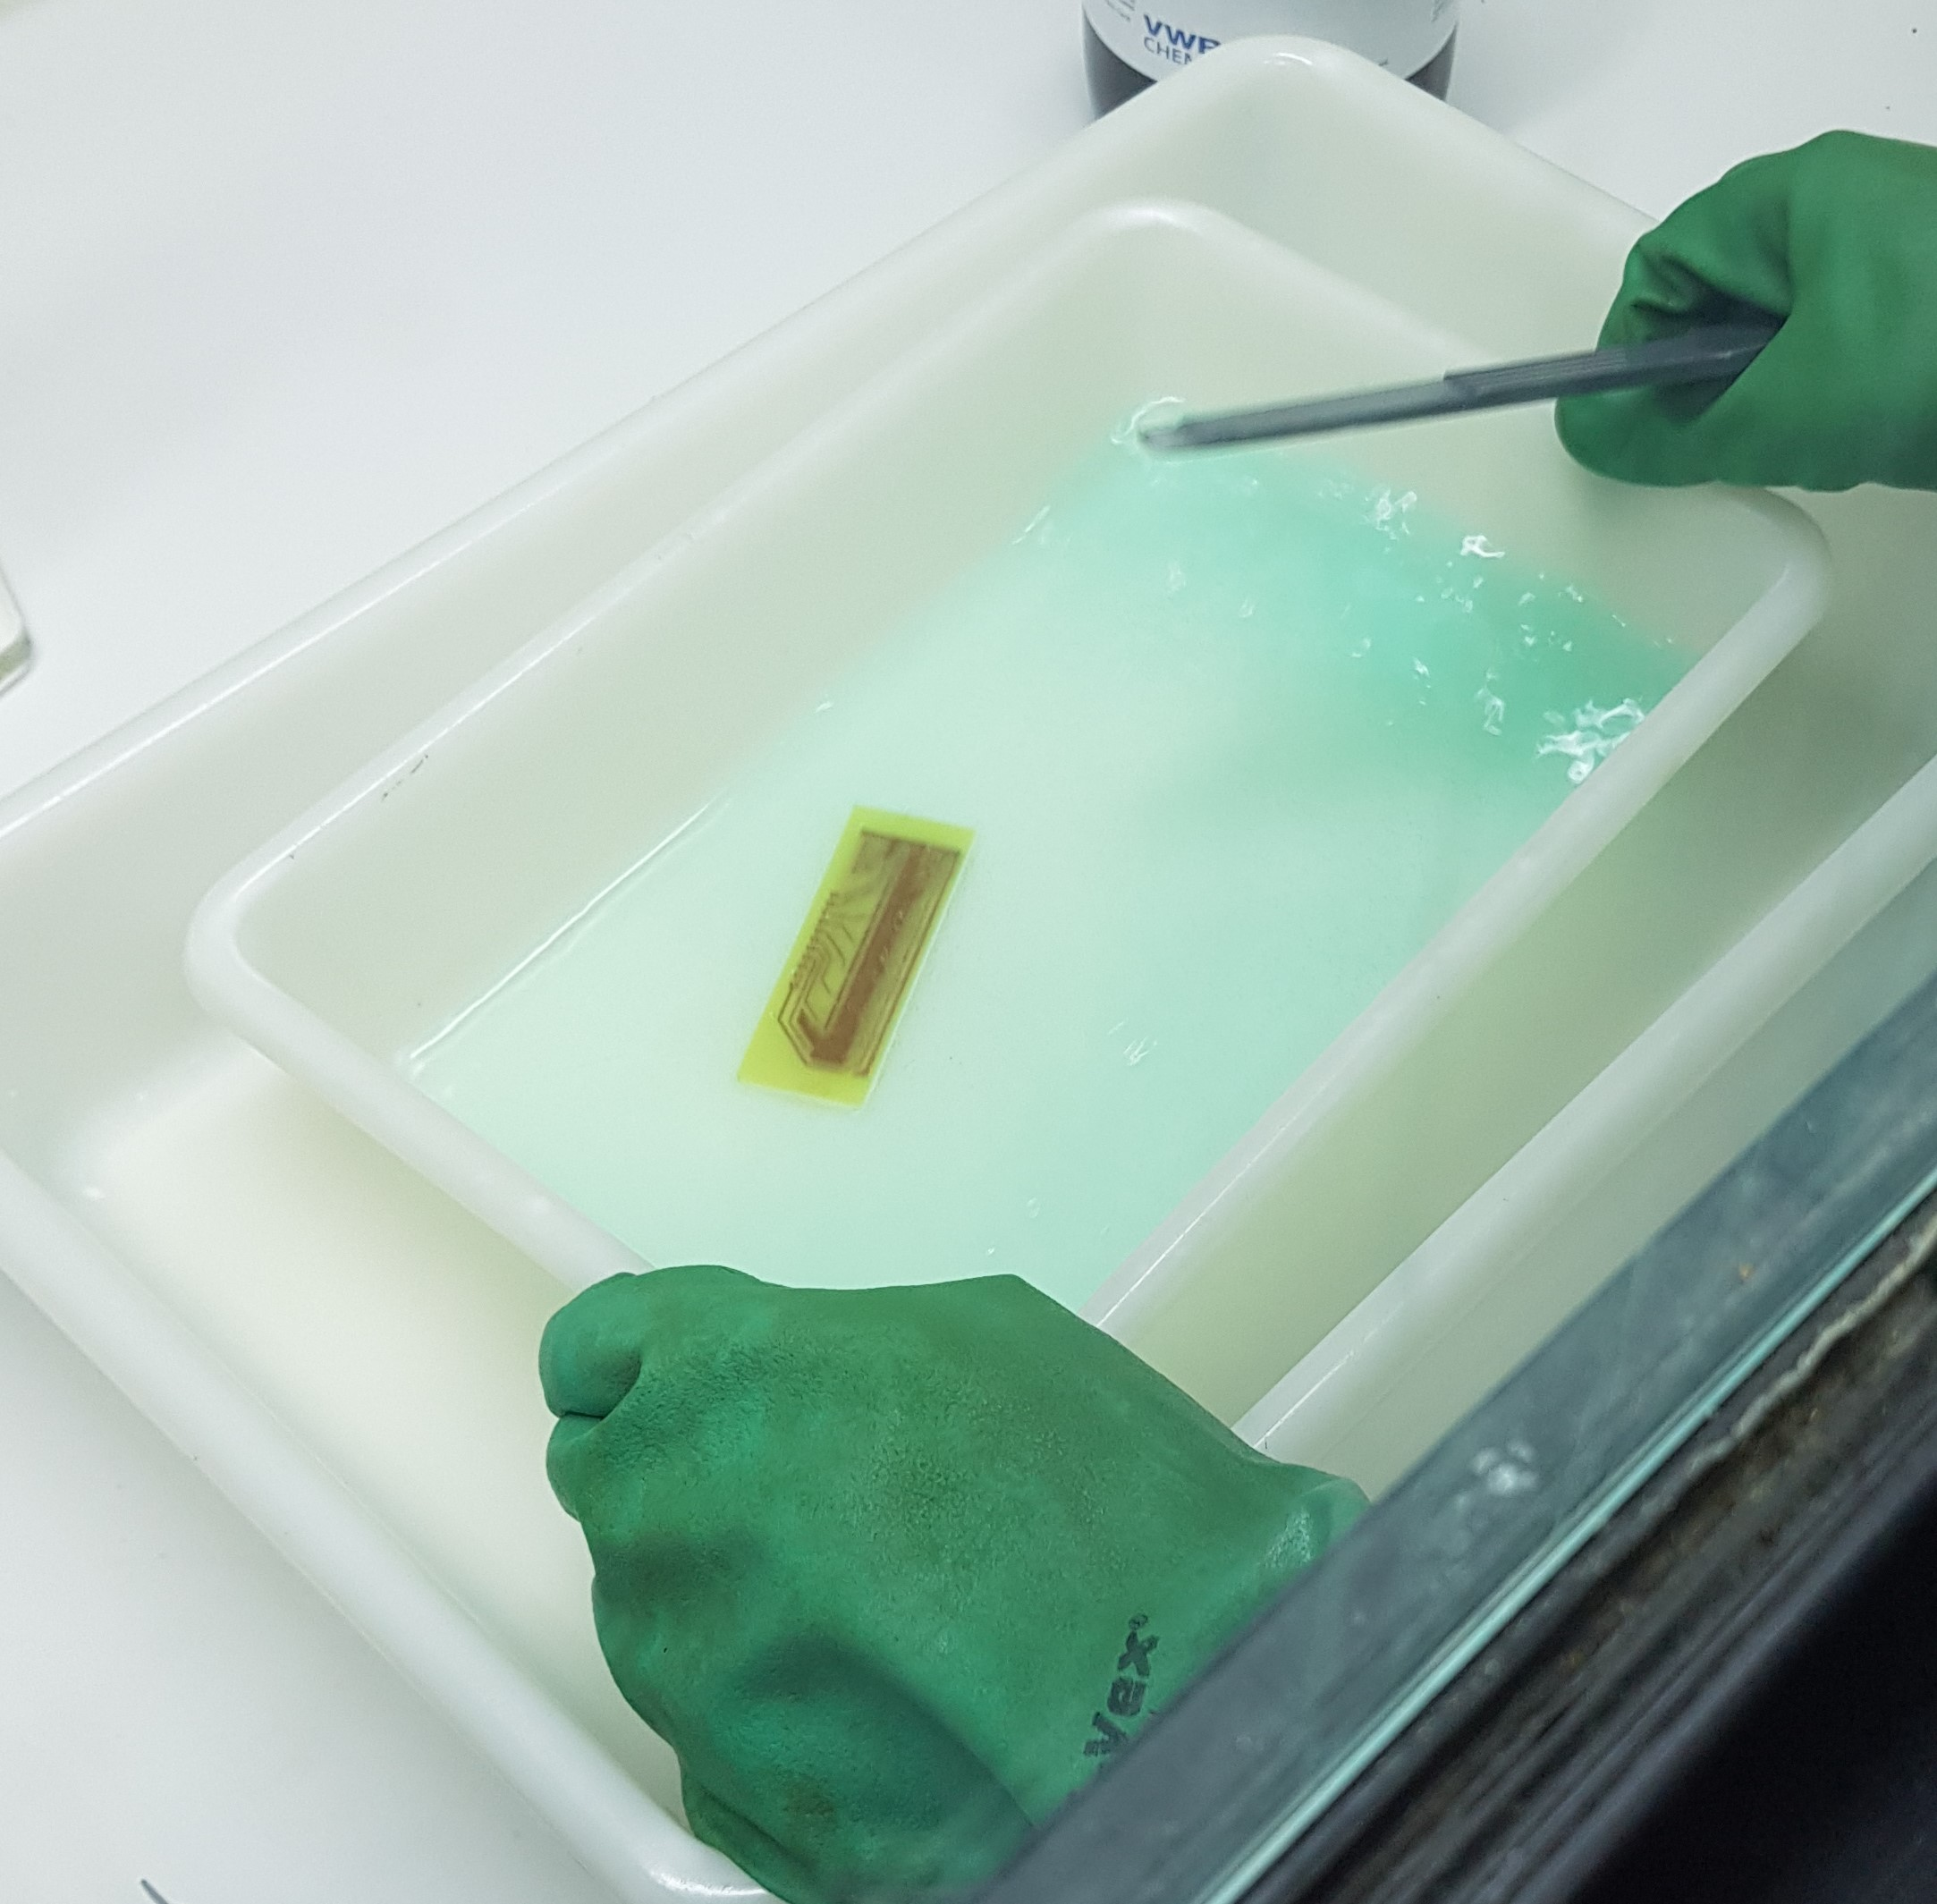
\includegraphics[width=.49\textwidth, height=\acidHeight]{figures/process_etching_progress.jpg}}
	\subfigure[End of the PCB copper cleaning with acid]{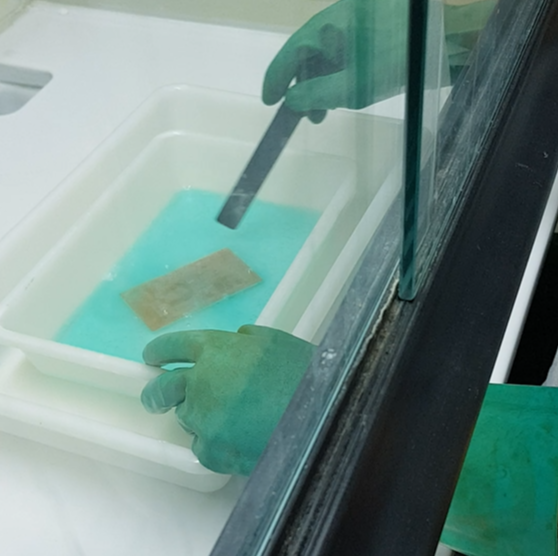
\includegraphics[width=.49\textwidth, height=\acidHeight]{figures/process_etching_complete.png}}
	\caption{PCB acid cleaning}
	\label{fig:acid}
\end{figure}
%
The admixtures ratio described in the \autoref{section:prep} is a fast mix, so you have to be moving all the time the copper plate until it seems similar to the PCBs shown in the \autoref{fig:pcbs}. It is really important to be careful with the tiny details and do not exceed the time of the copper plate in the acid mix.

After take it out of the acid mix, clean the copper plate with abundant water and dry it with some paper. The result should seem like the two sides of two PCBs of the \autoref{fig:pcbs}.
%
\begin{figure}[H]
	\centering
	\subfigure[Top view]{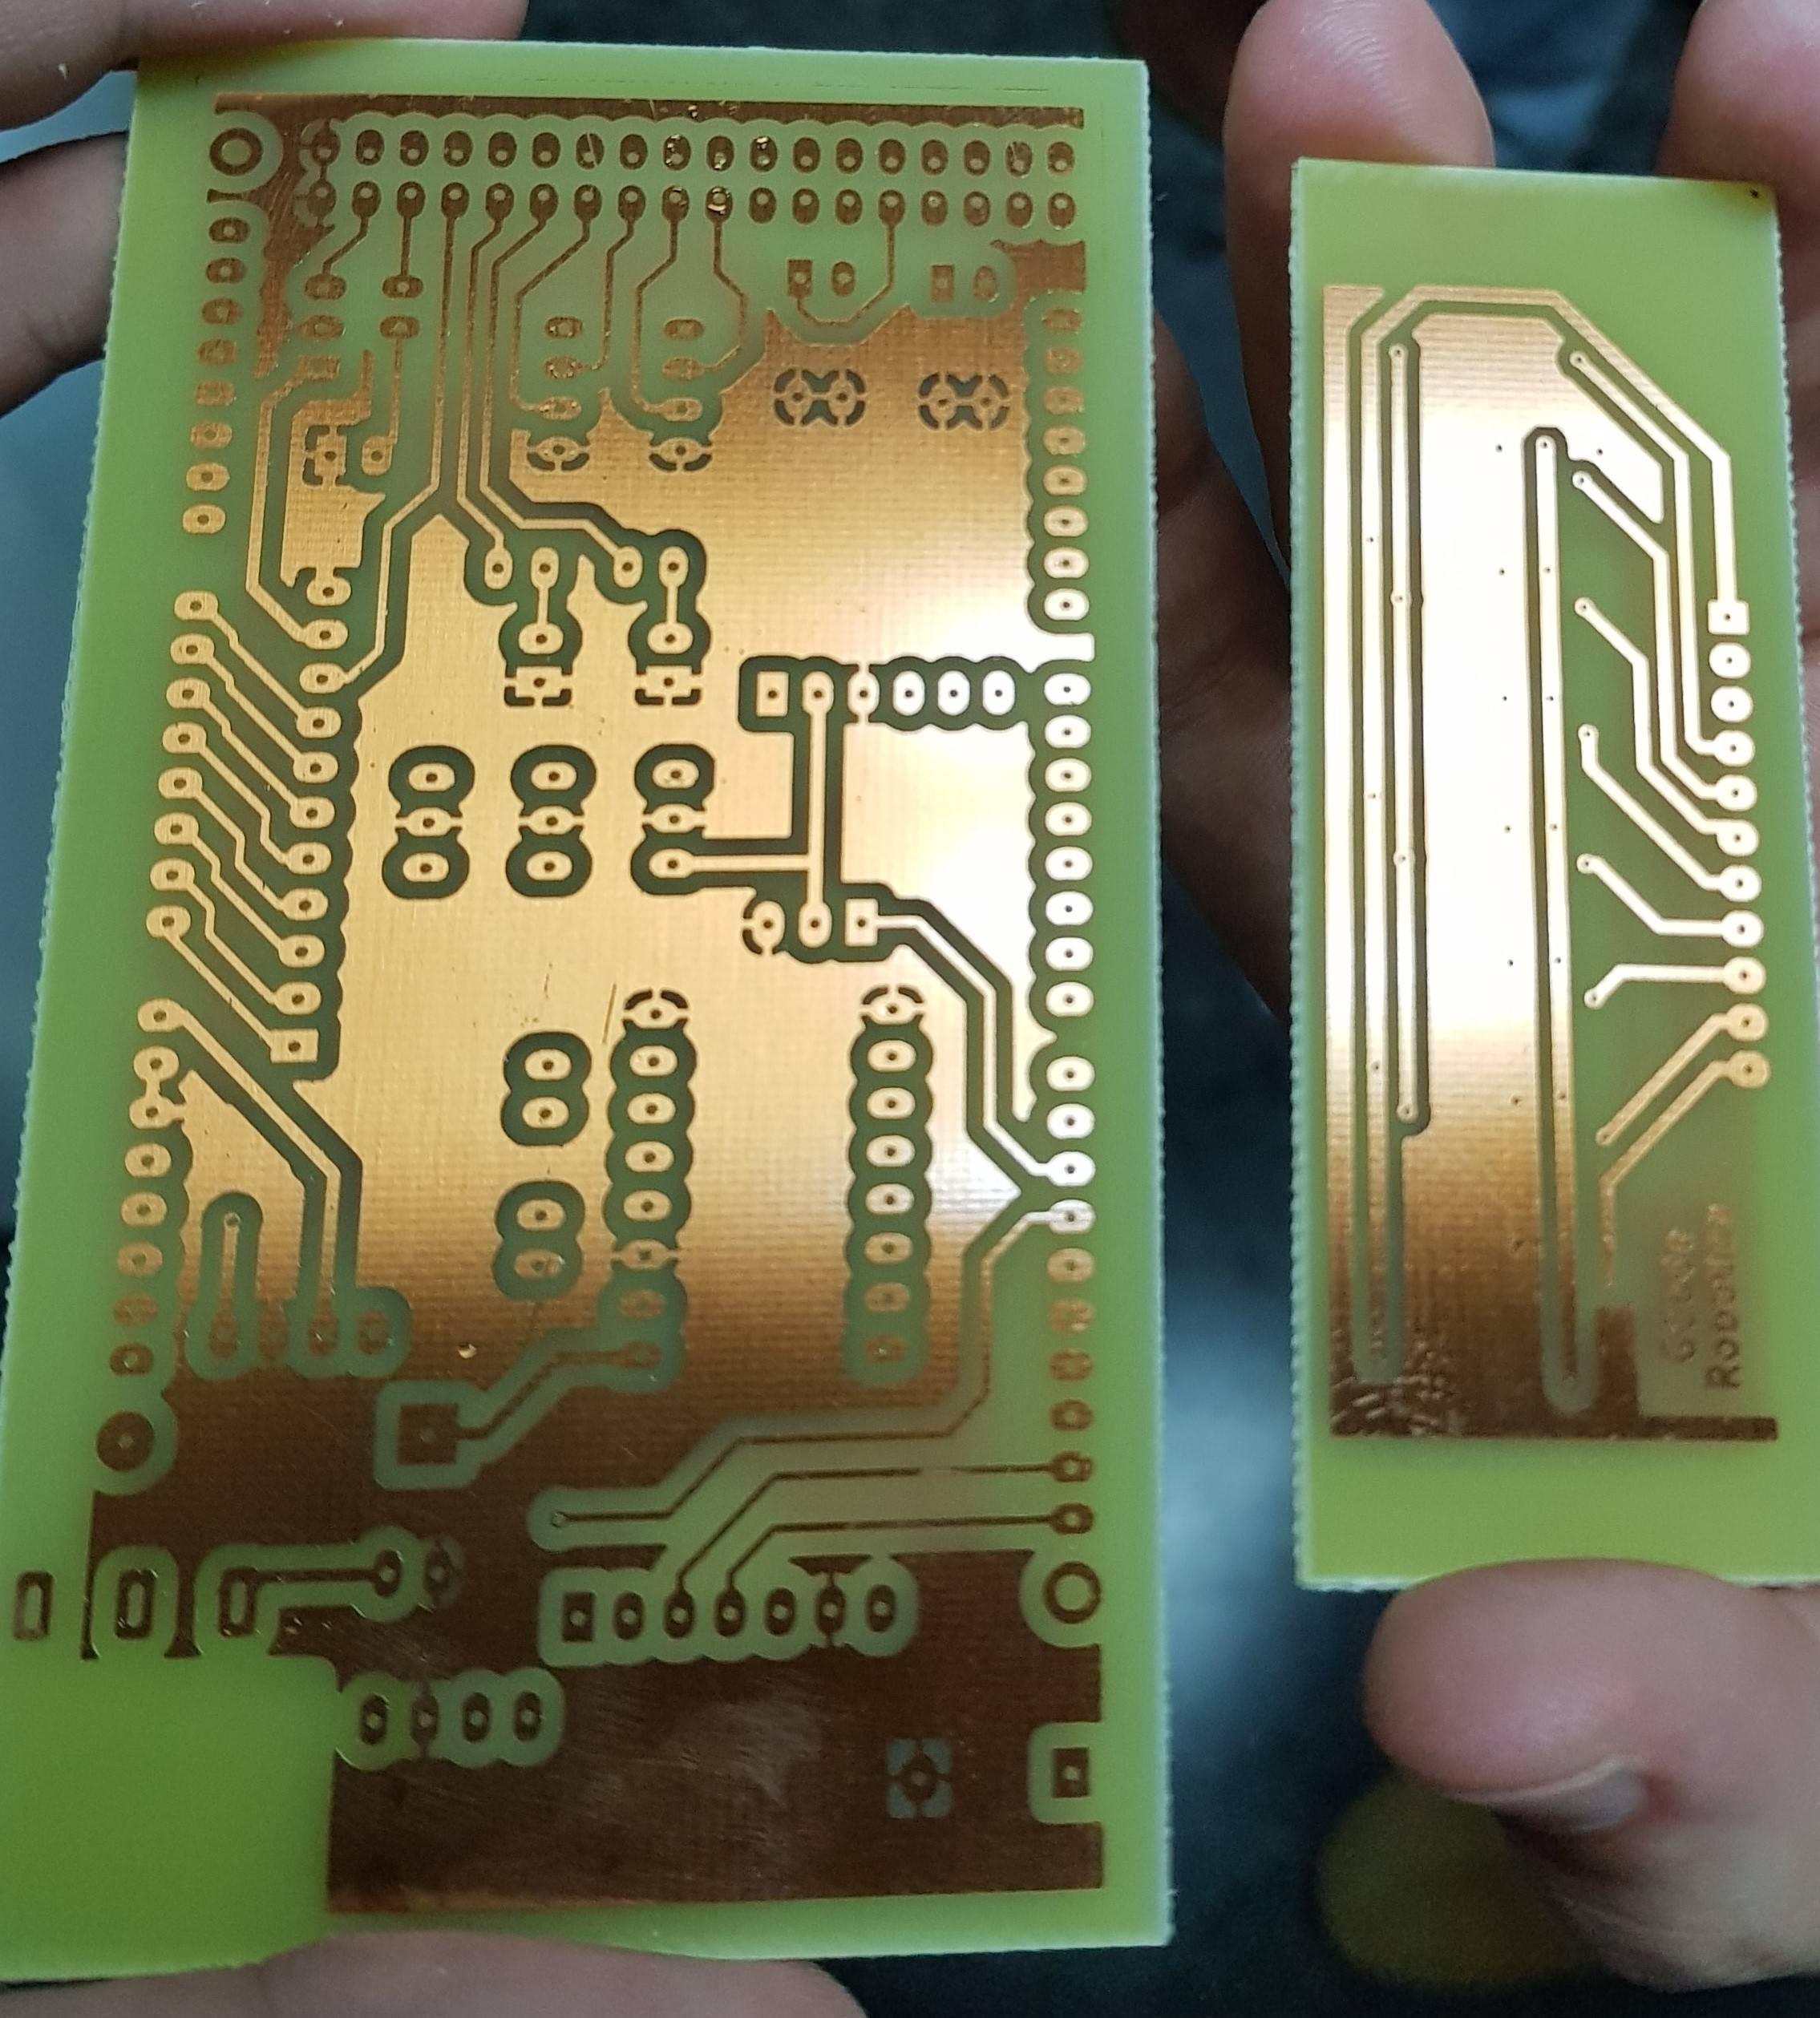
\includegraphics[width=.49\textwidth, height=\pcbsHeight]{figures/pcb_result_etched_top.jpg}}
	\subfigure[Bottom view]{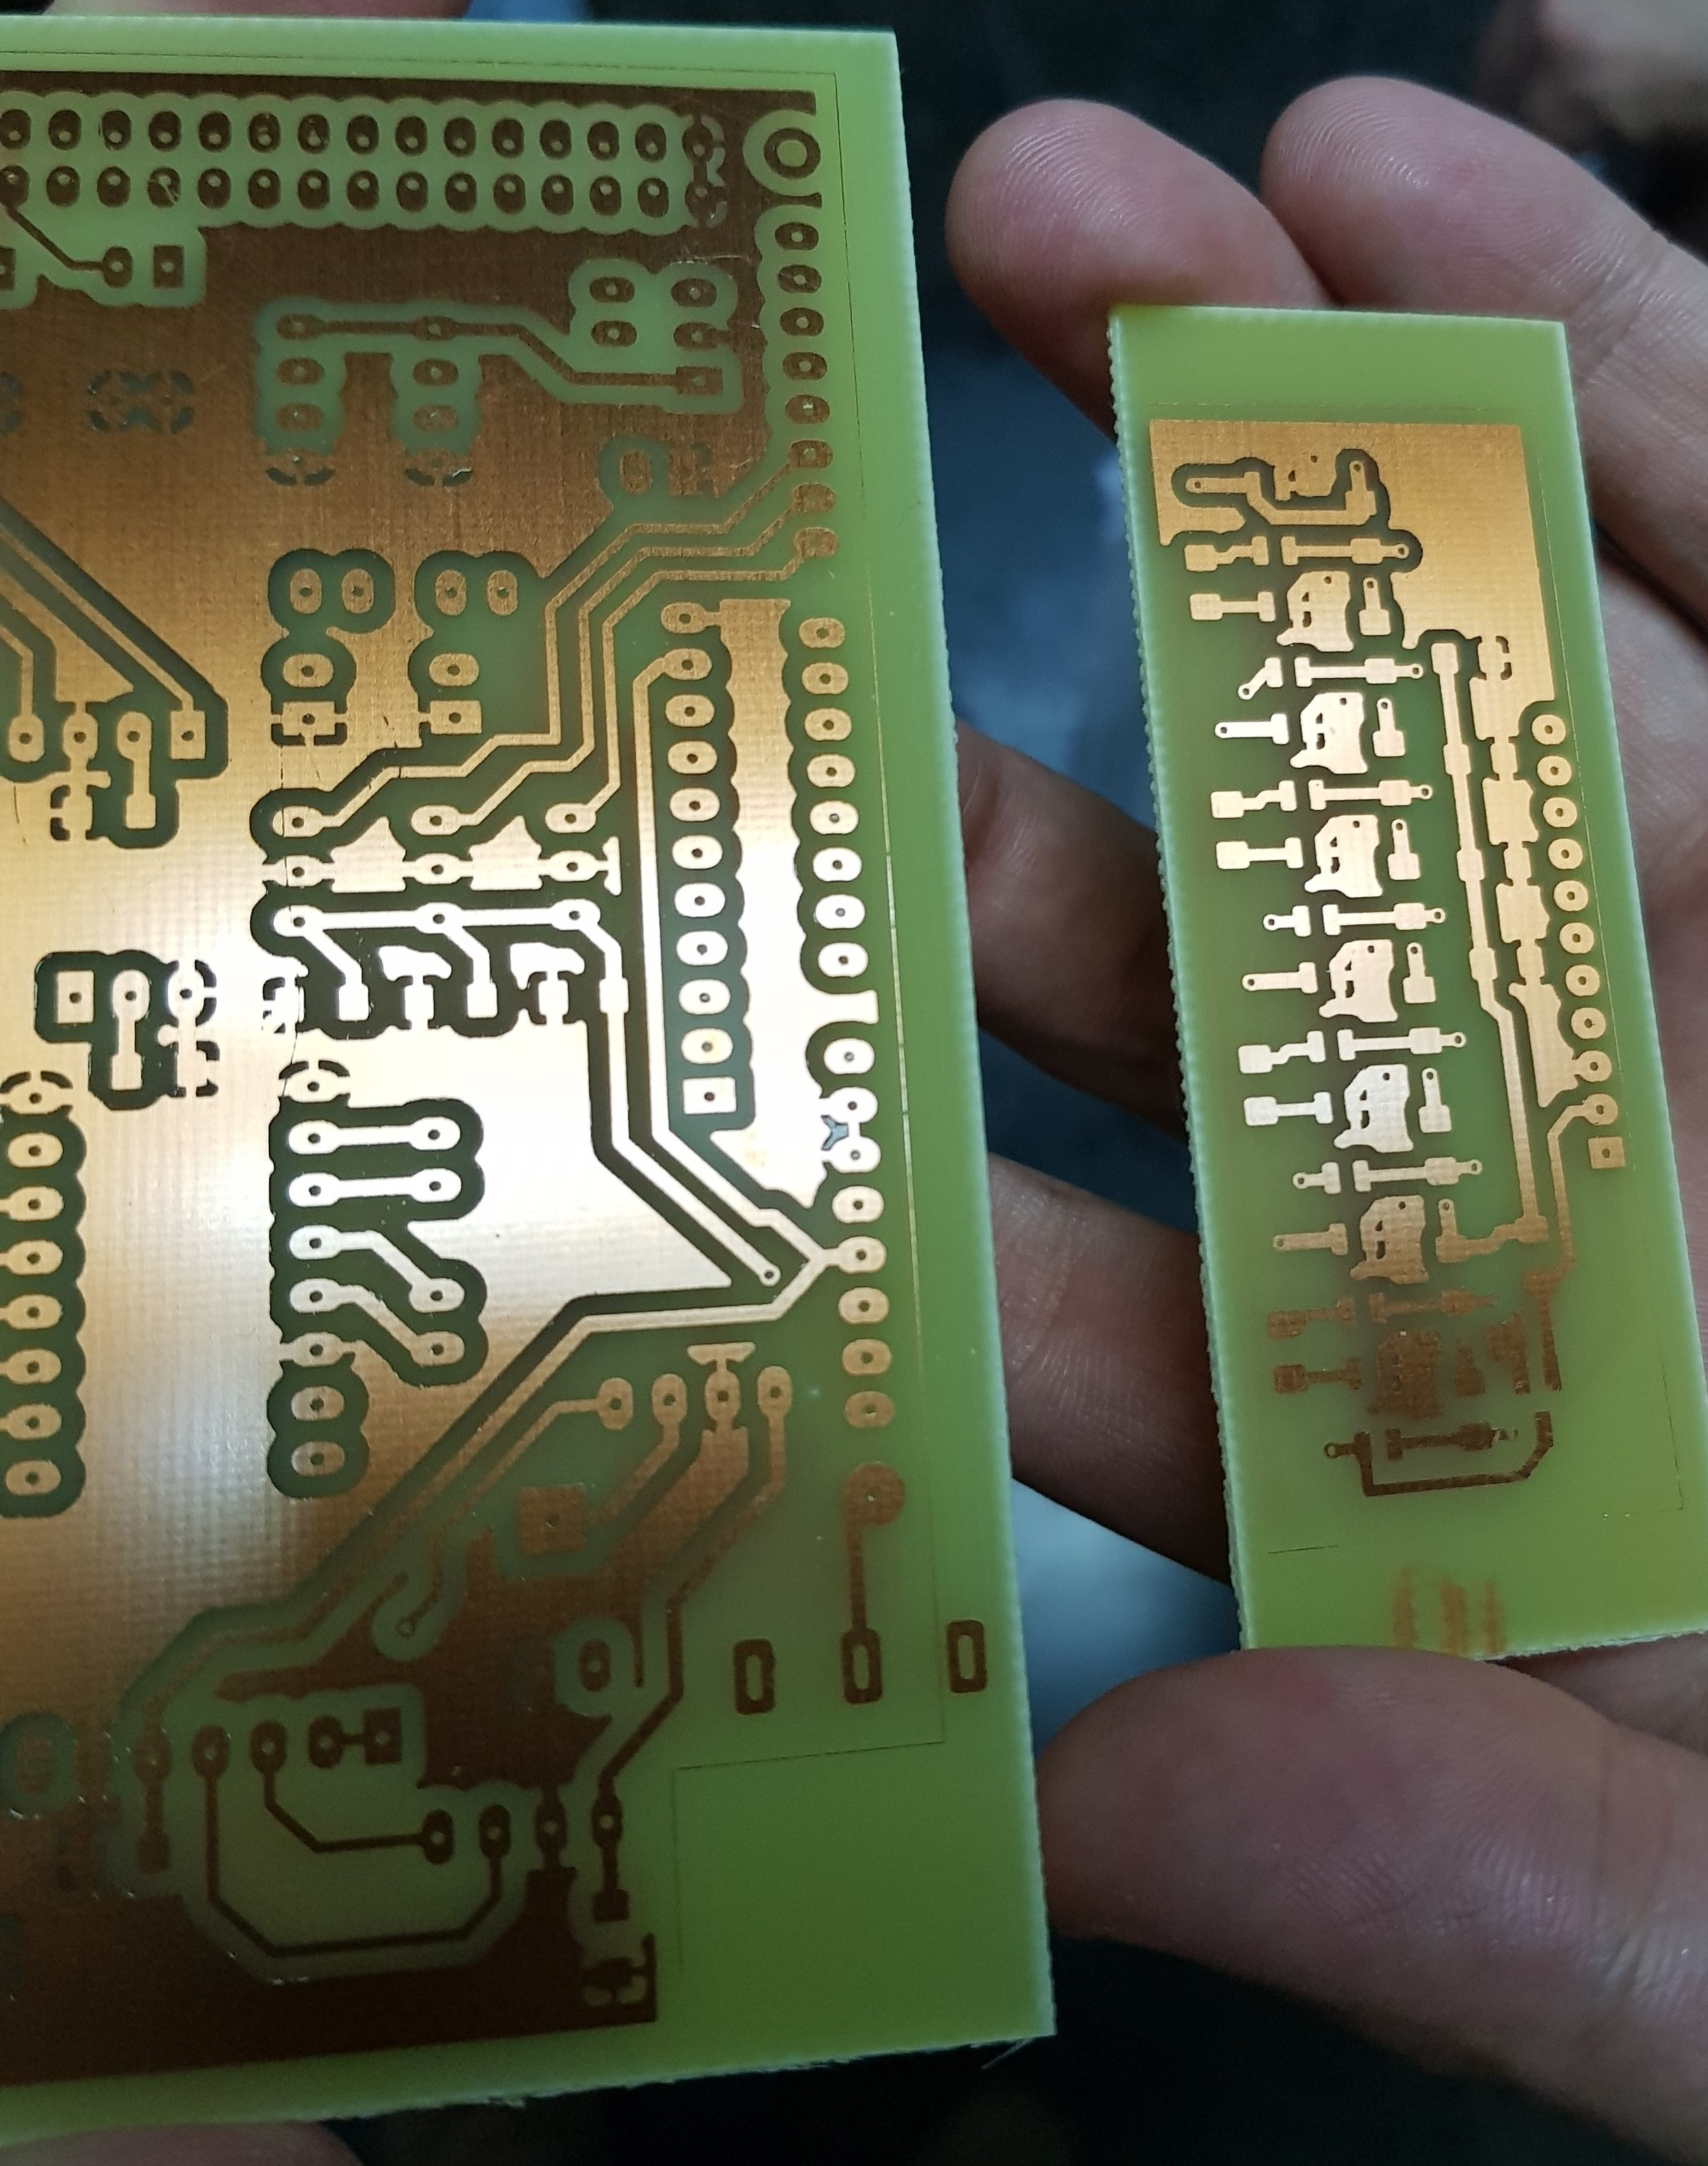
\includegraphics[width=.49\textwidth, height=\pcbsHeight]{figures/pcb_result_etched_bottom.jpg}}
	\caption{Top and bottom view of a pair of finished PCBs}
	\label{fig:pcbs}
\end{figure}
%
Whereas that caustic soda can be reused several times, the acid mix has to be stored in a container suitable for this purpose and removed by some company able to do it. A container example is shown in the \autoref{fig:containers}.
%
\begin{figure}[H]
	\centering
	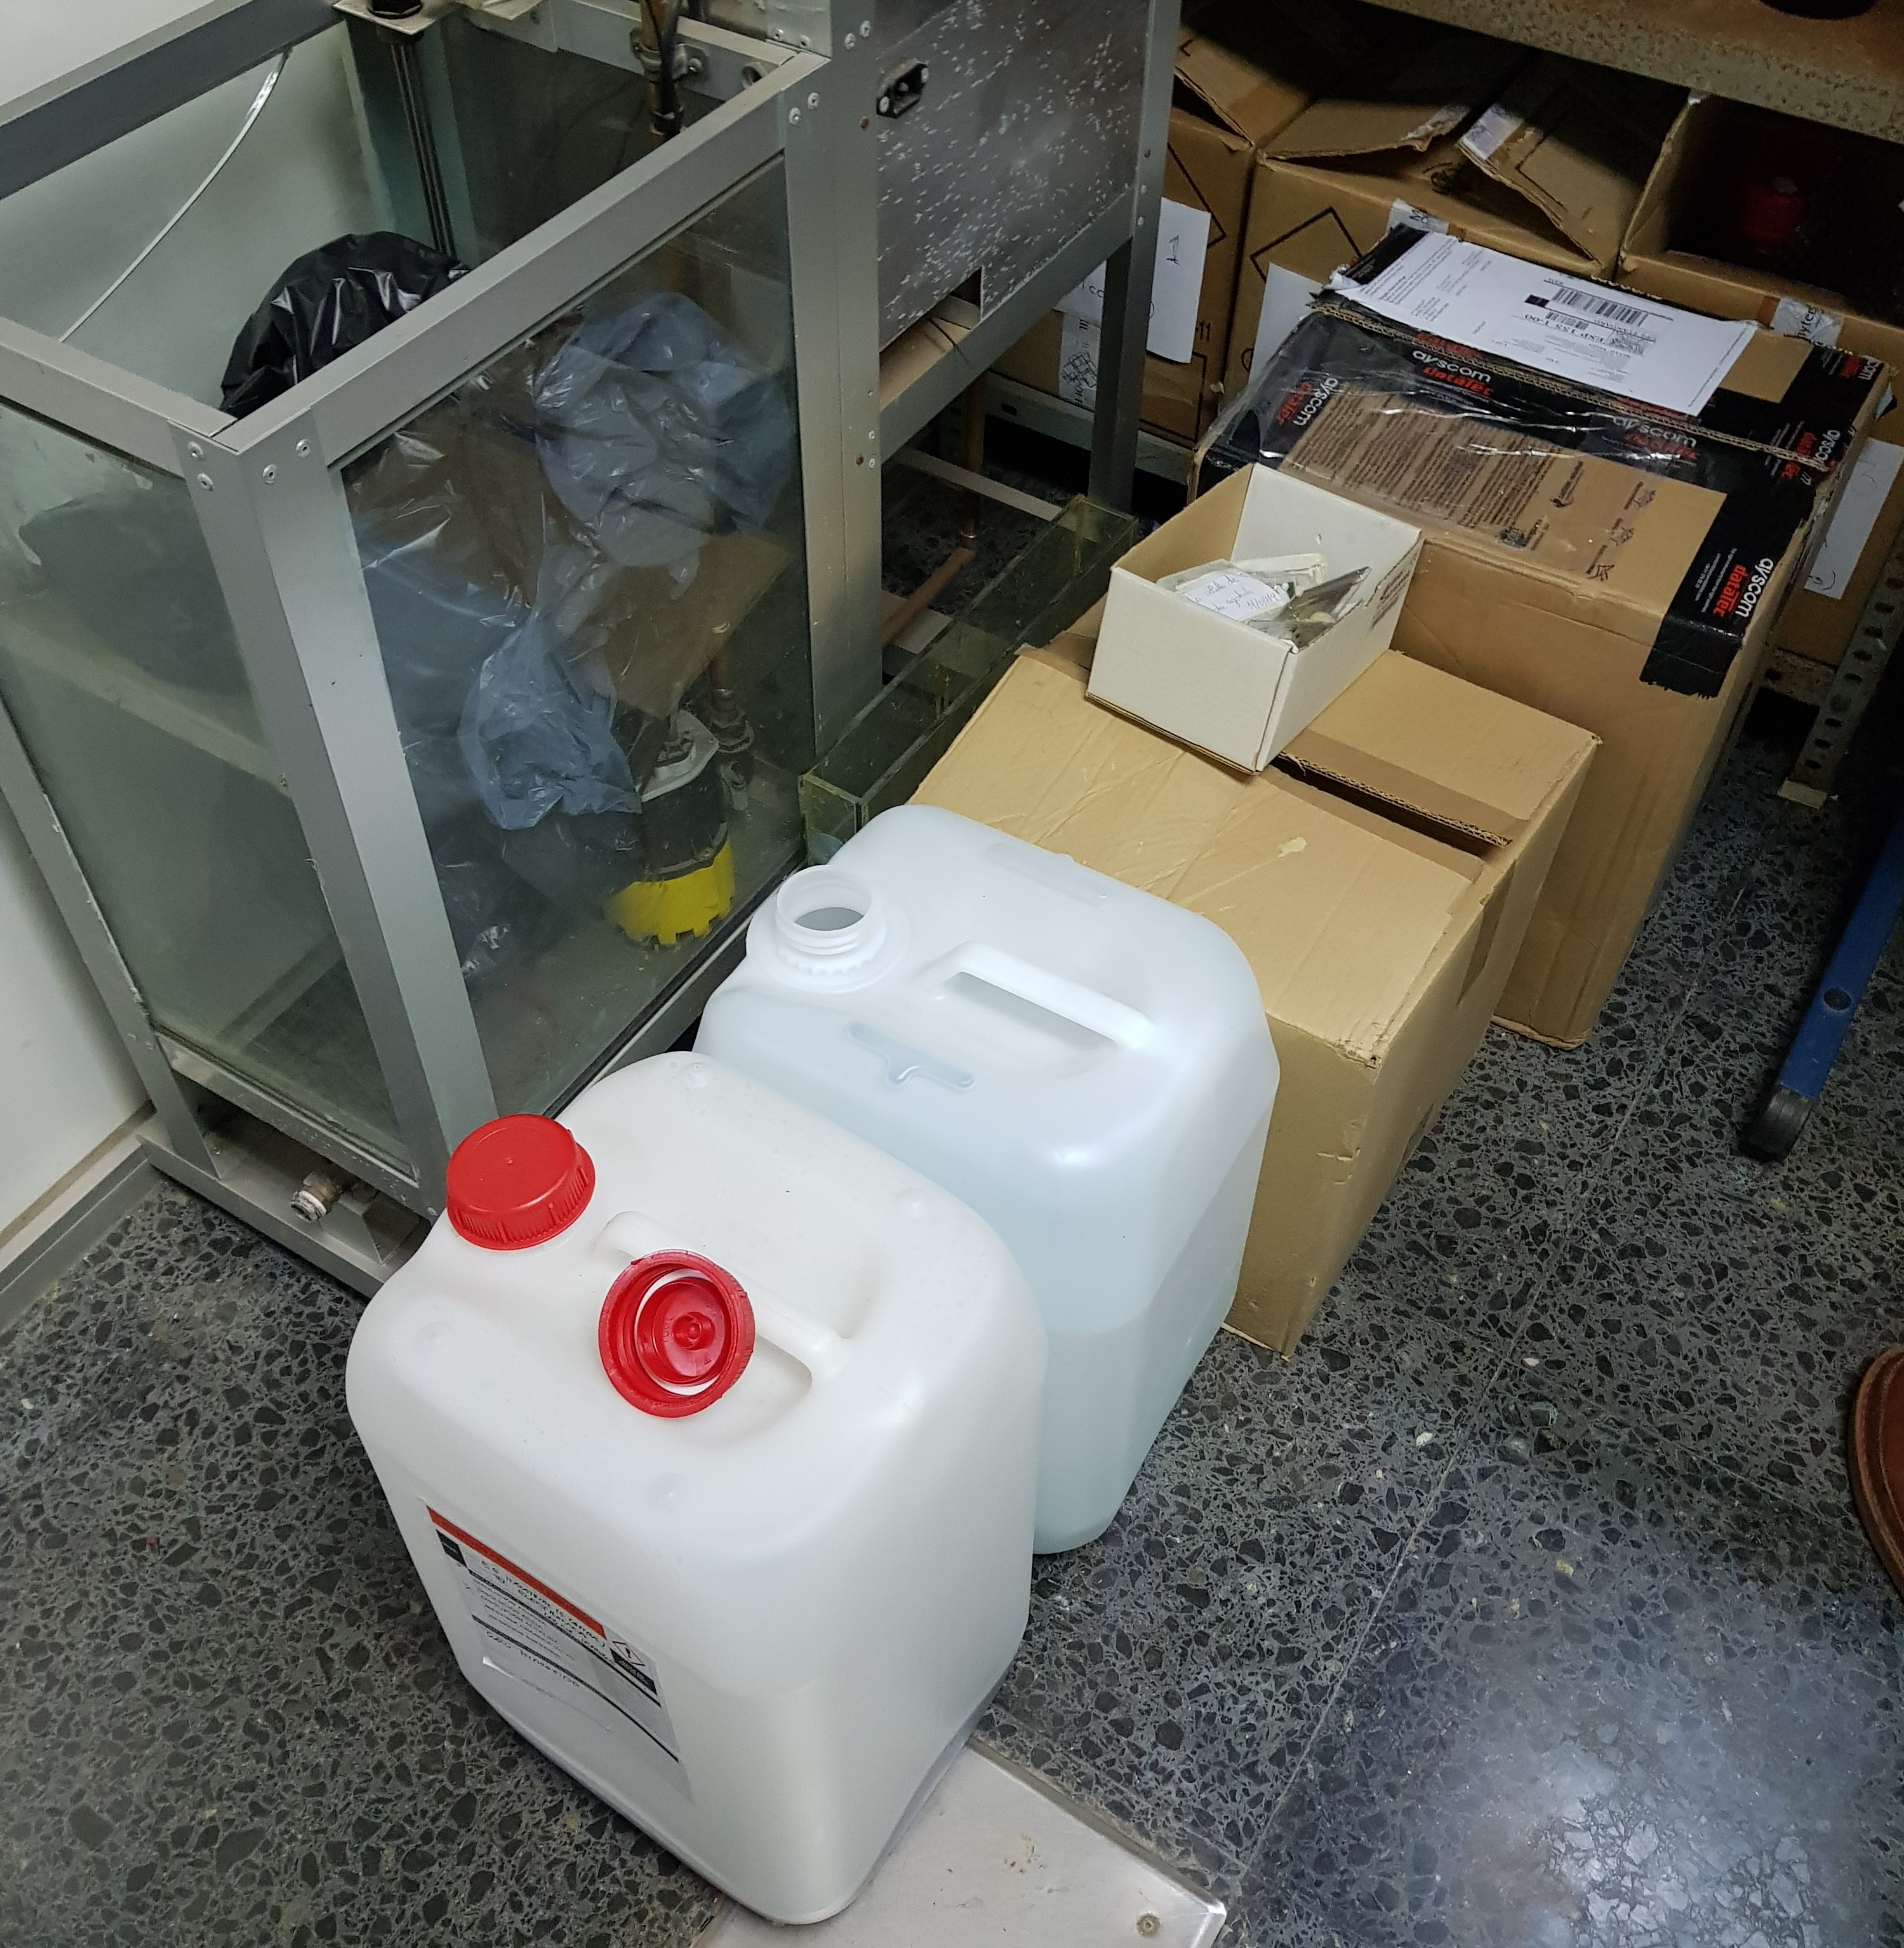
\includegraphics[width=.49\textwidth]{figures/process_waste_containers.jpg}
	\caption{Acid residues containers}
	\label{fig:containers}
\end{figure}
%
%
\section{Post-processing}
%
Good job! If you have reached this point you already have a beautiful home-made PCB. Now, it is time to adjust more the size of this PCB, if the previous use of the shear machine has not reached a desirable quality grade. The shear machine can used again as shown in the \autoref{fig:postciz} or use a Dremel with a suitable cut disk\footnote{Remember to use protection gloves and glasses}.
%
\begin{figure}[H]
	\centering
	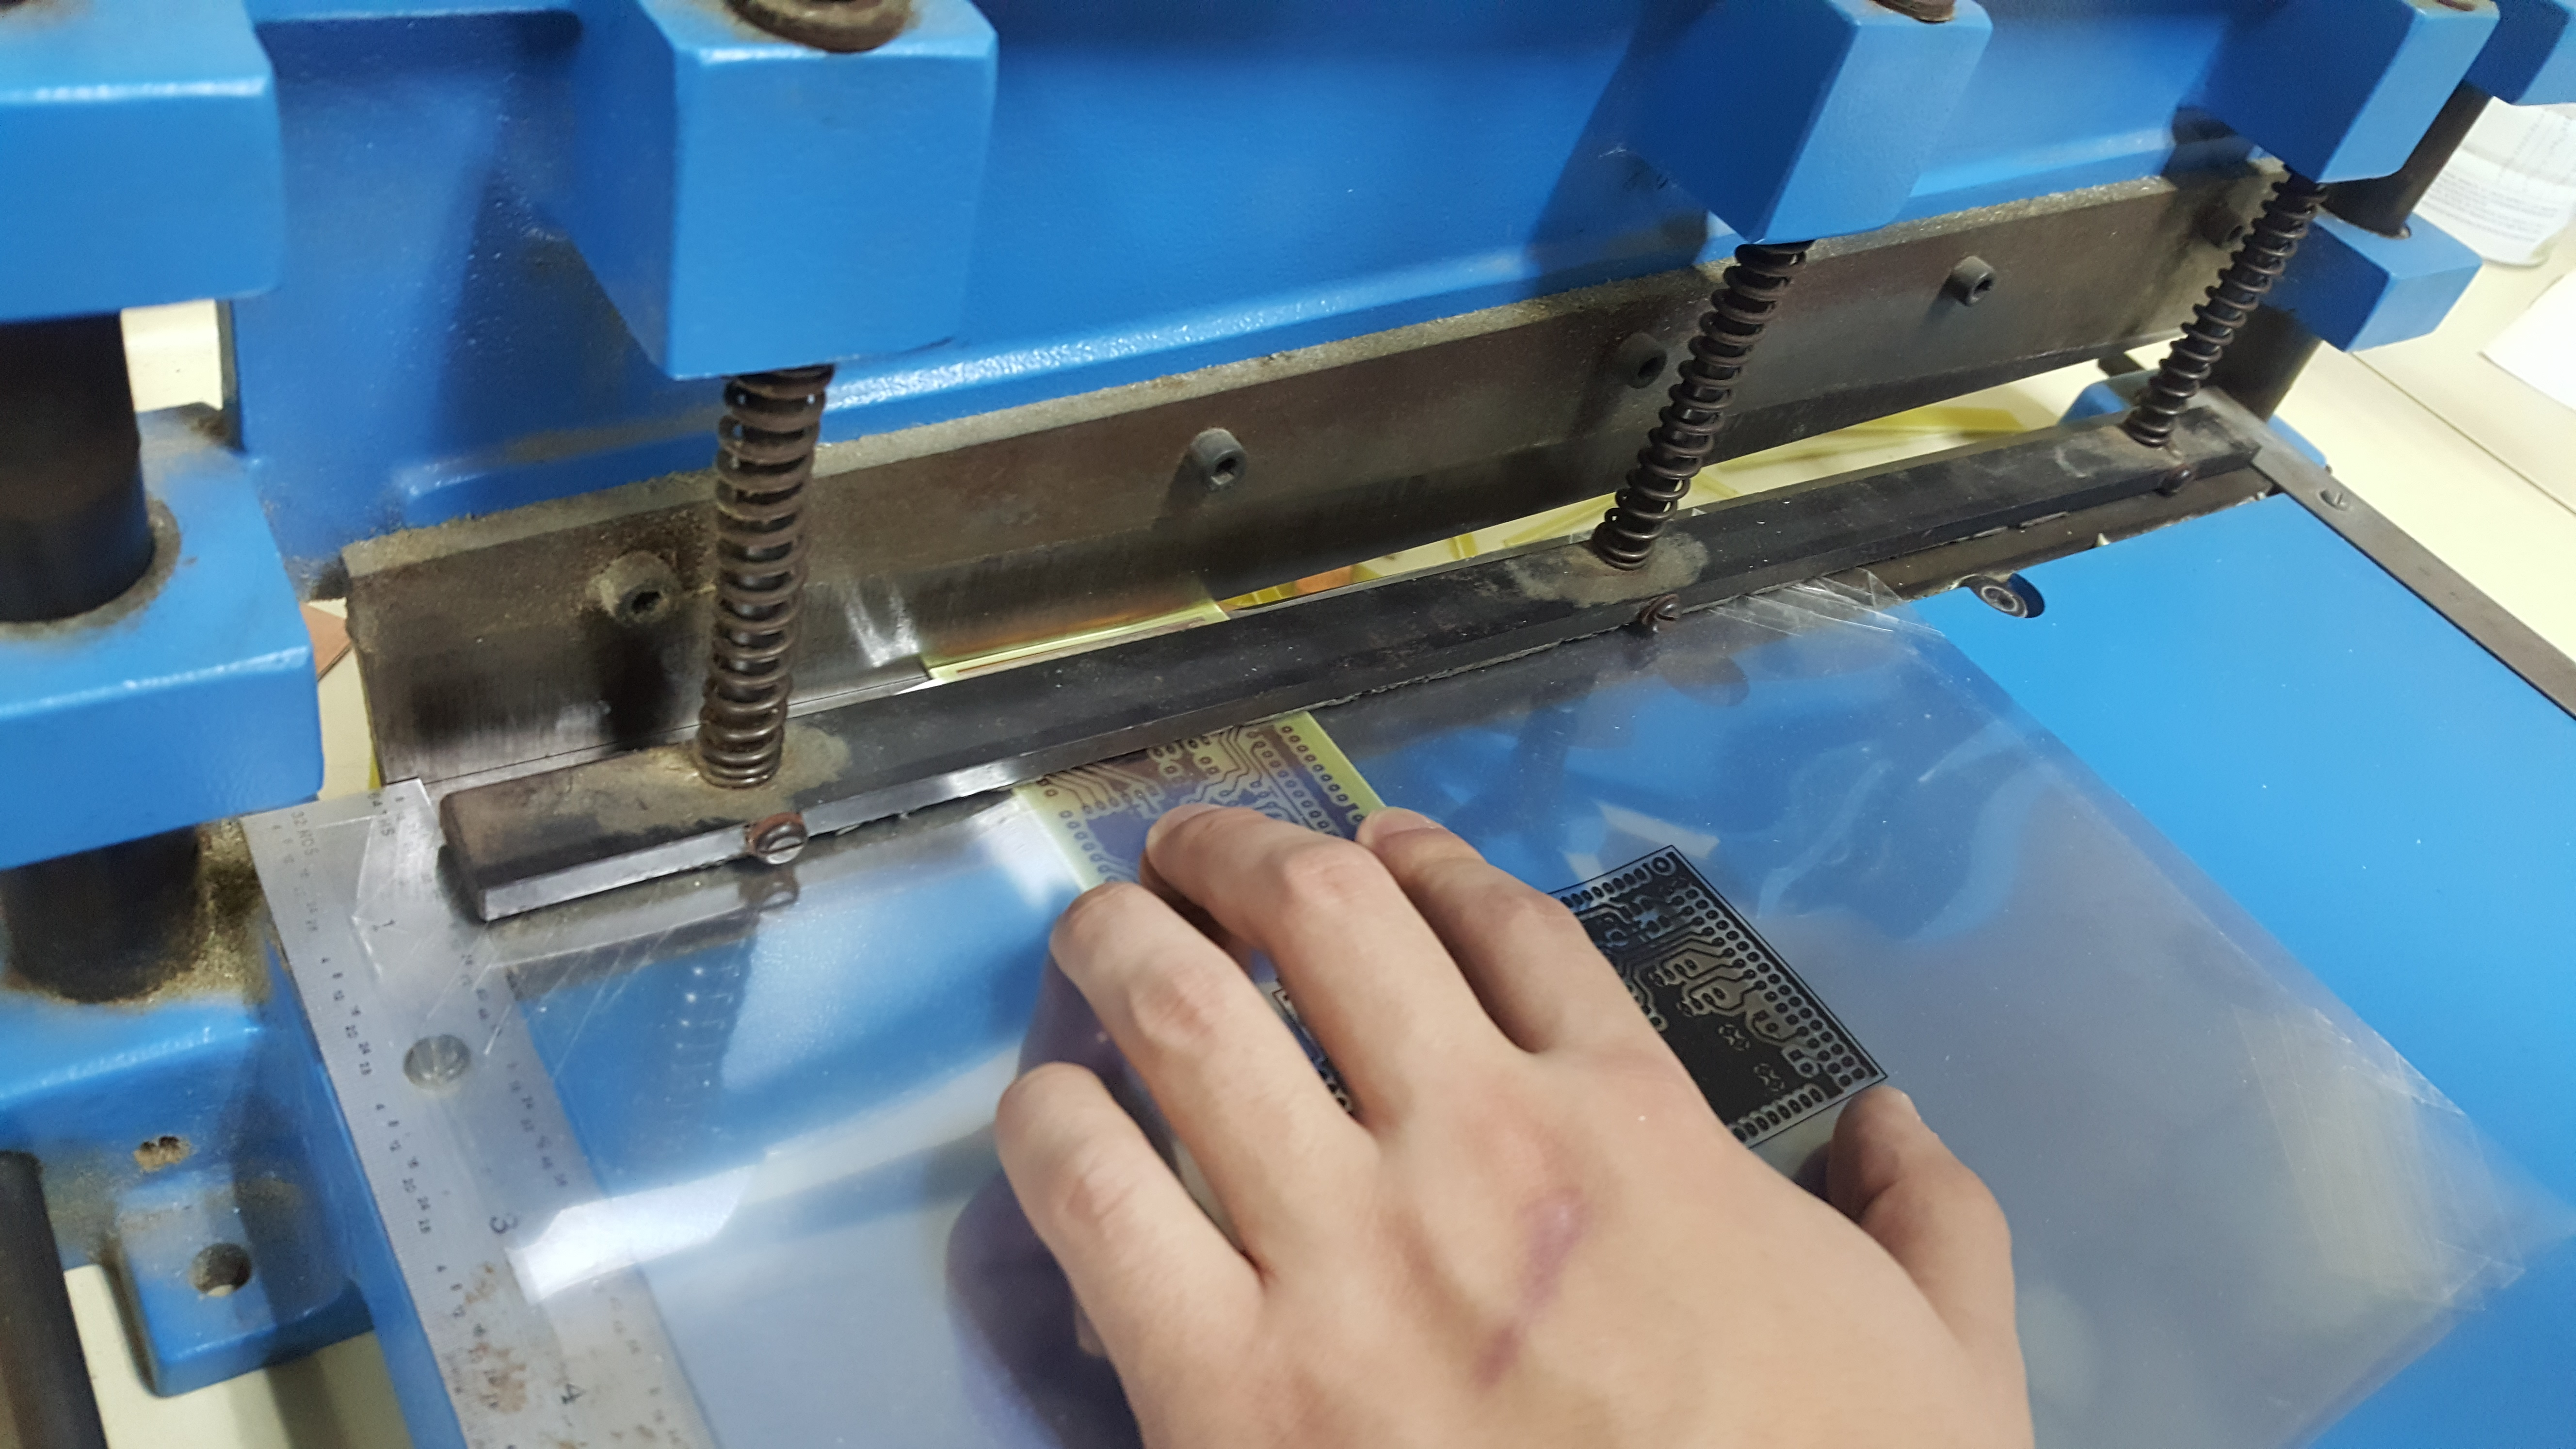
\includegraphics[width=.49\textwidth]{figures/process_cutting_post_etching.jpg}
	\caption{Shear machine with the PCB finished placed}
\label{fig:postciz}
\end{figure}
%
Then, clean the PCB with acetone to clean the copper protection remains. Furthermore, it is usual to have to do some drills in the PCB. It can be made for Through Hole Technology (THT) components, vias or restraint holes, among others. With this on mind, it is a good idea to use a fixed vertical Dremel with a suitable drill diameter as shown in the \autoref{fig:taladrico}. It is recommendable to use some material as wood as PCB support in order to not scratch the PCB traces. In the \autoref{fig:drill} is shown four team members hard drilling a PCB using this method.
%
\begin{figure}[H]
	\centering
	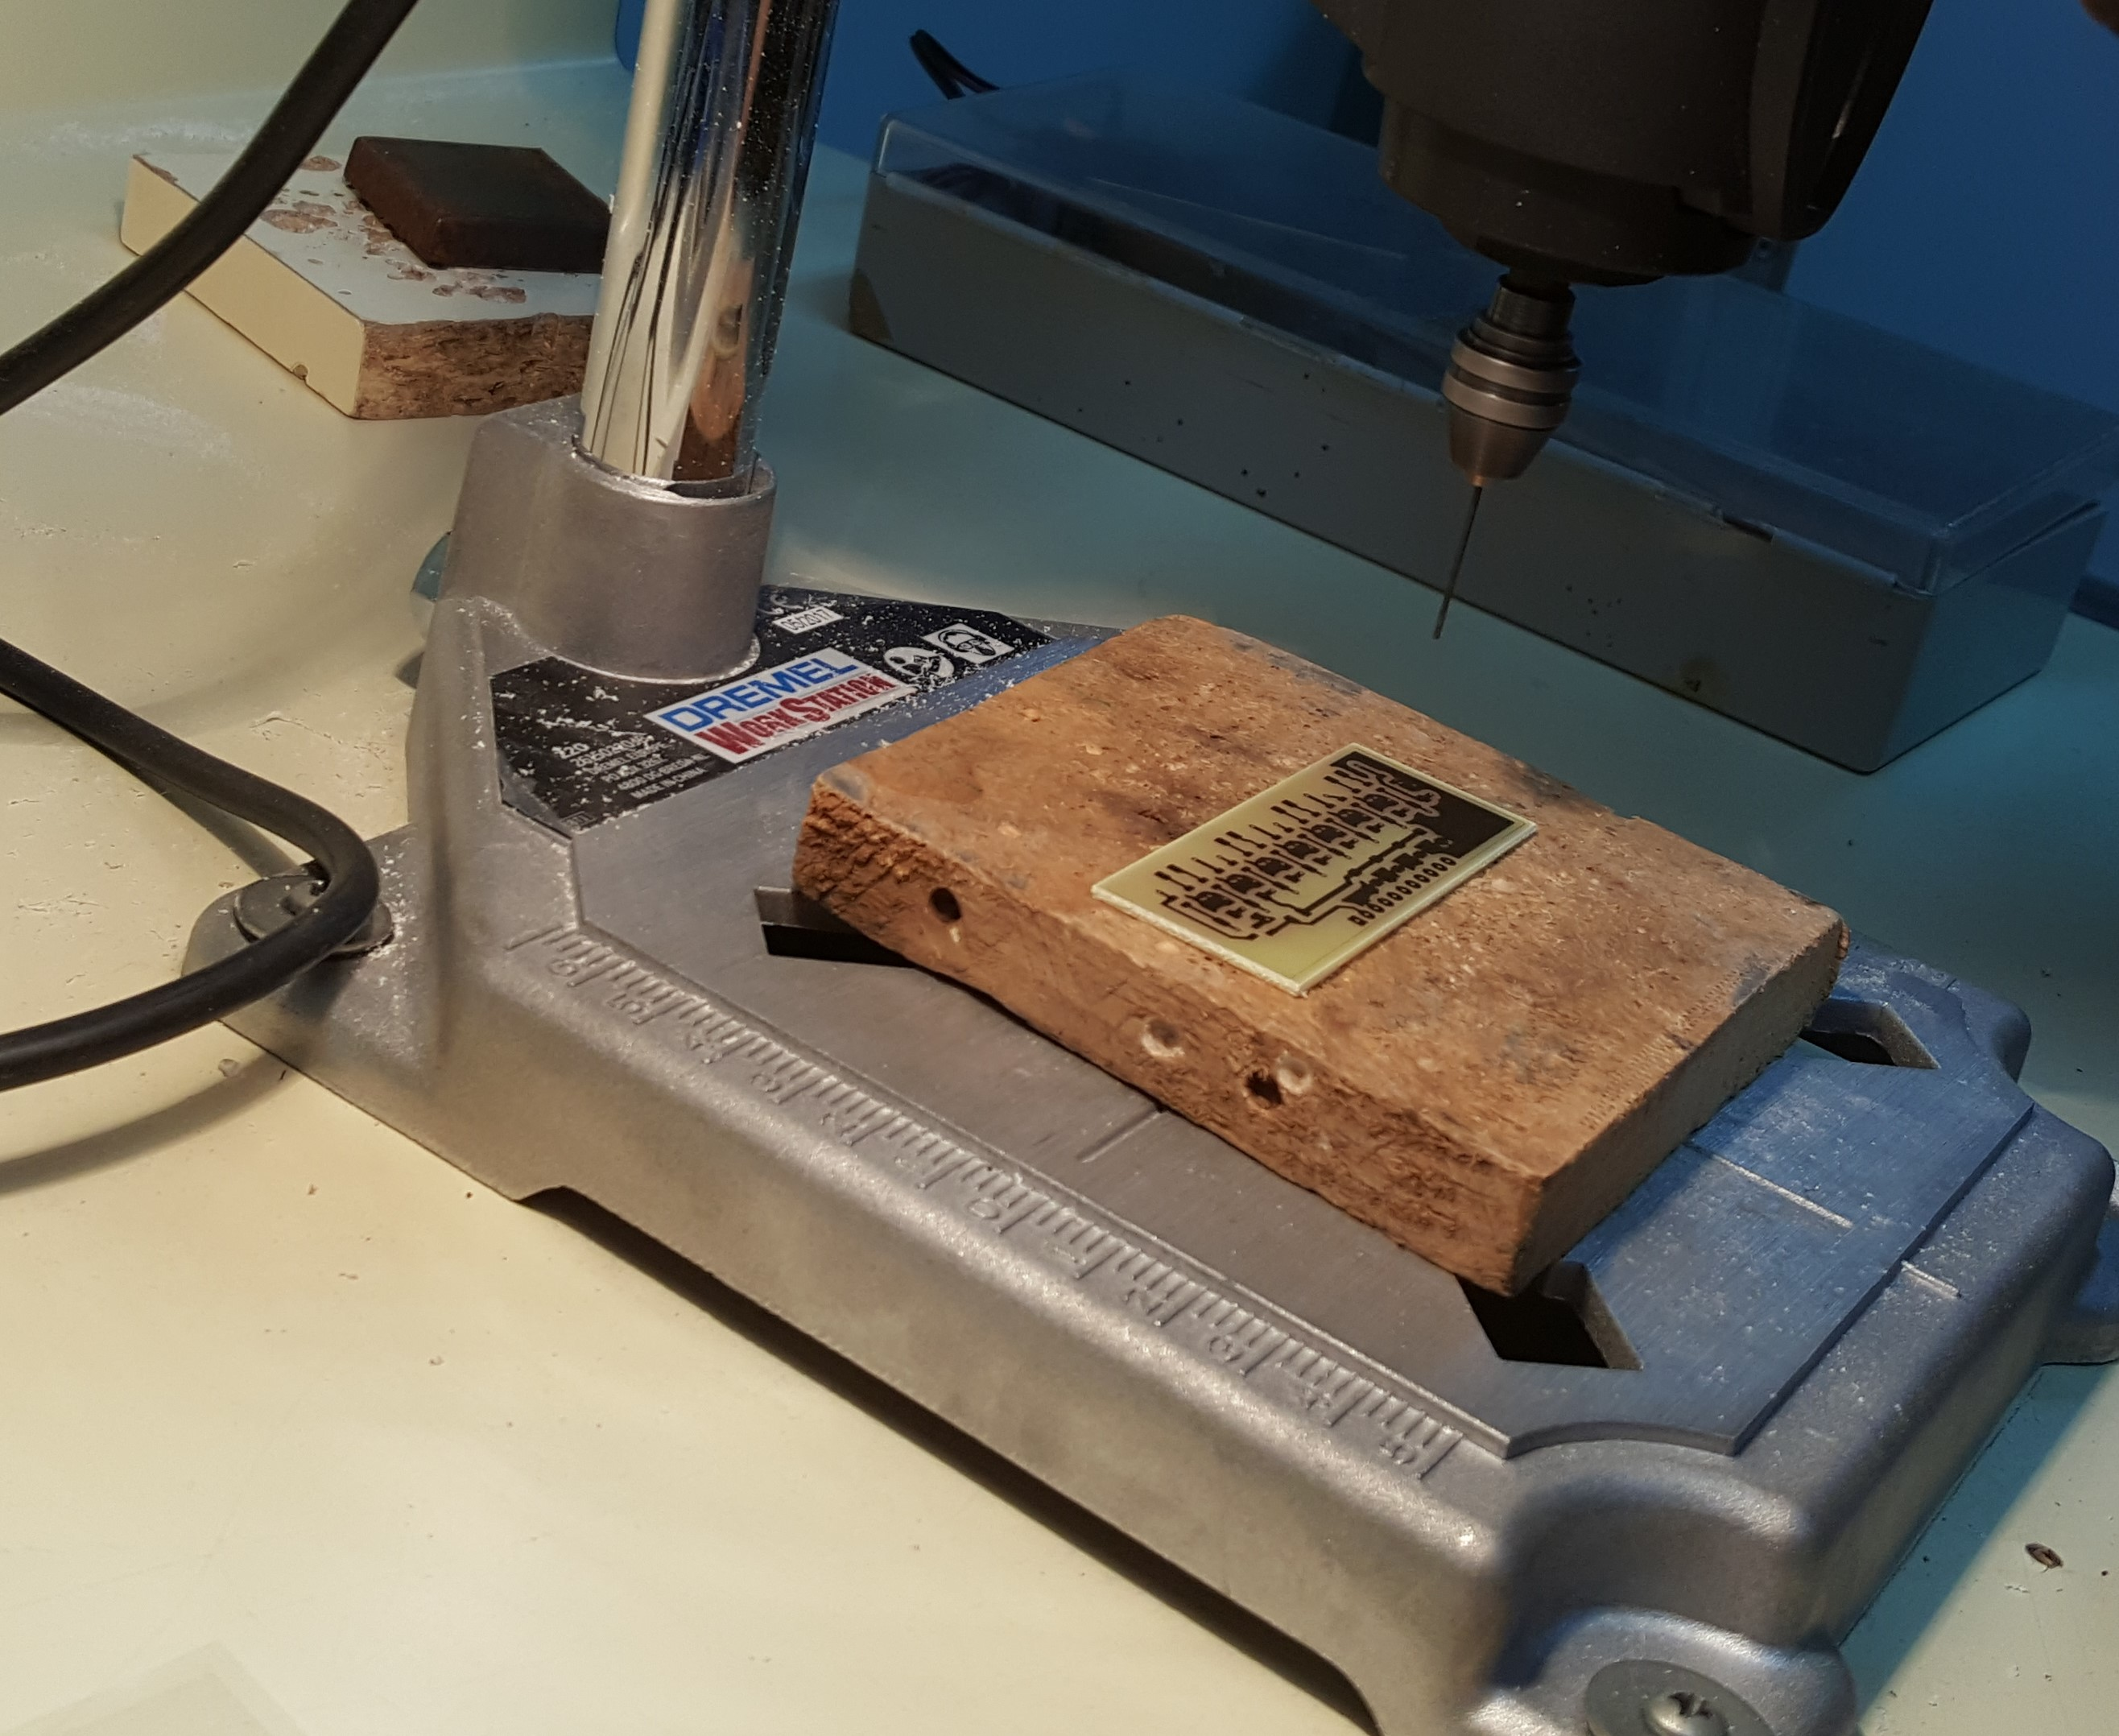
\includegraphics[width=.49\textwidth]{figures/process_drilling_setup.jpg}
	\caption{PCB placement for the drilling with a fixed Dremel}
	\label{fig:taladrico}
\end{figure}
%
%
\begin{figure}[H]
	\centering
	\subfigure[Mateo PCB super-drilling ]{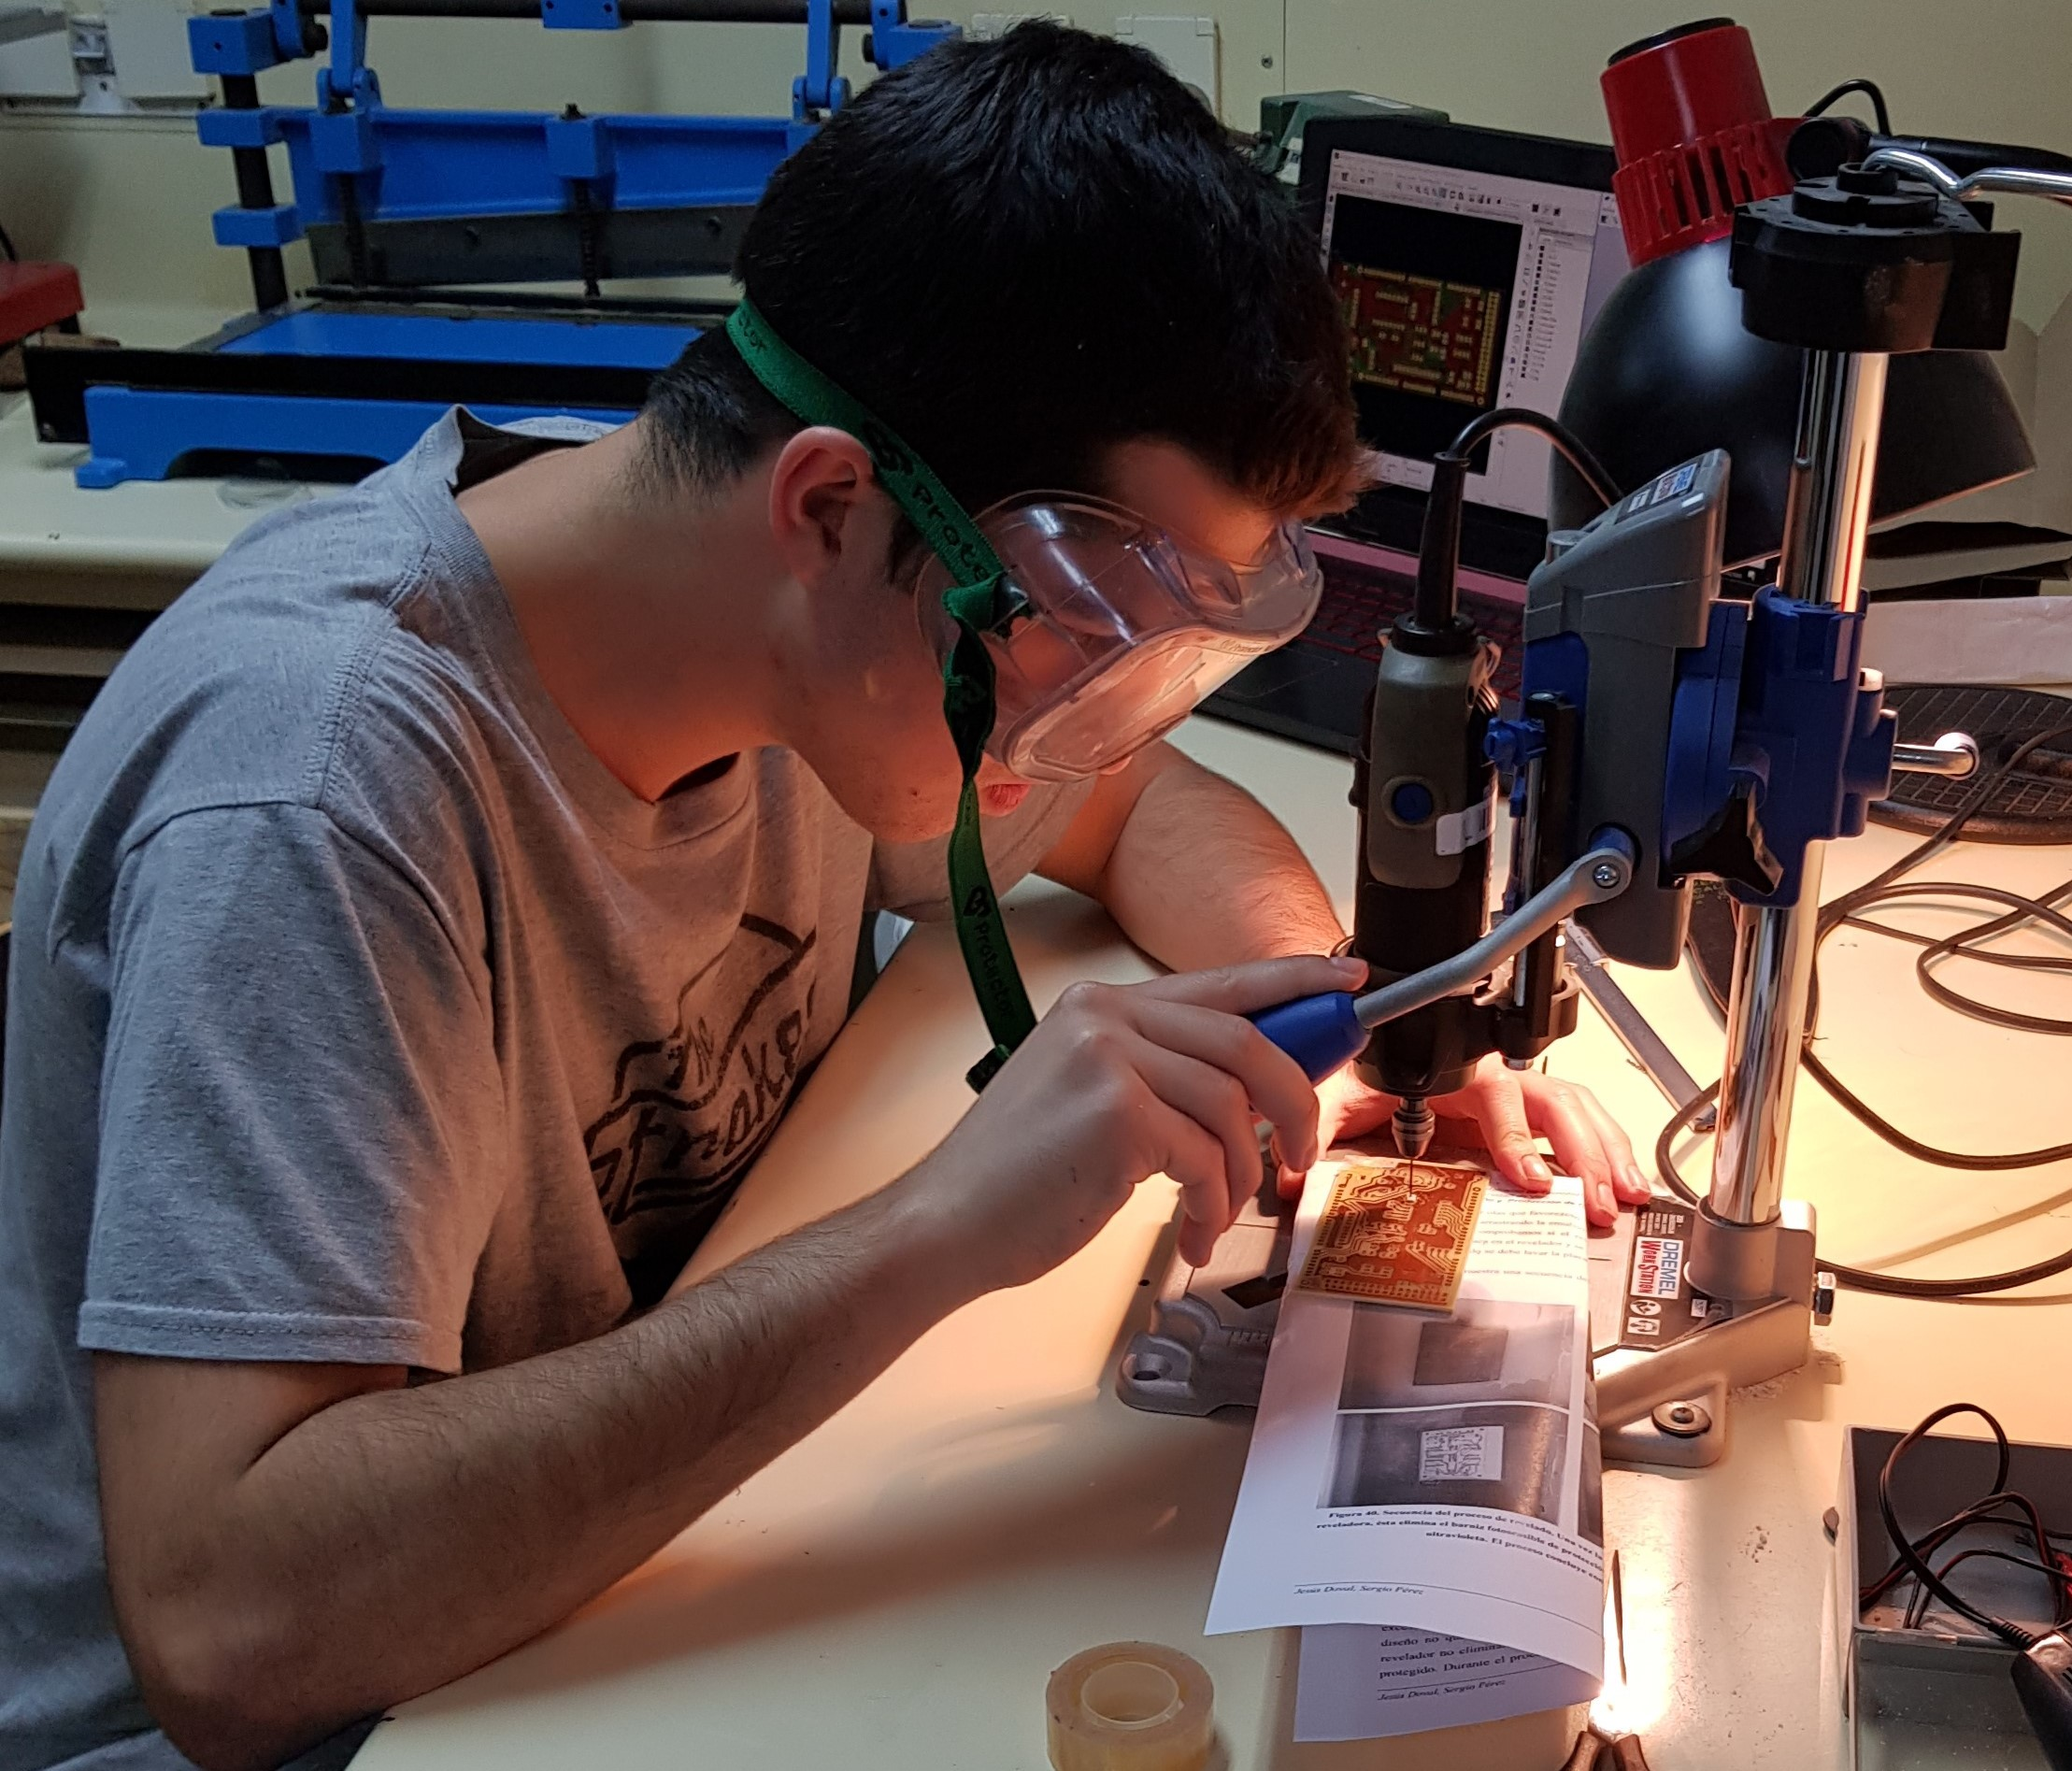
\includegraphics[width=.49\textwidth, height=\taladroHeight]{figures/process_drilling_team_mateo.jpg}}
	\subfigure[Elena PCB extra-drilling]{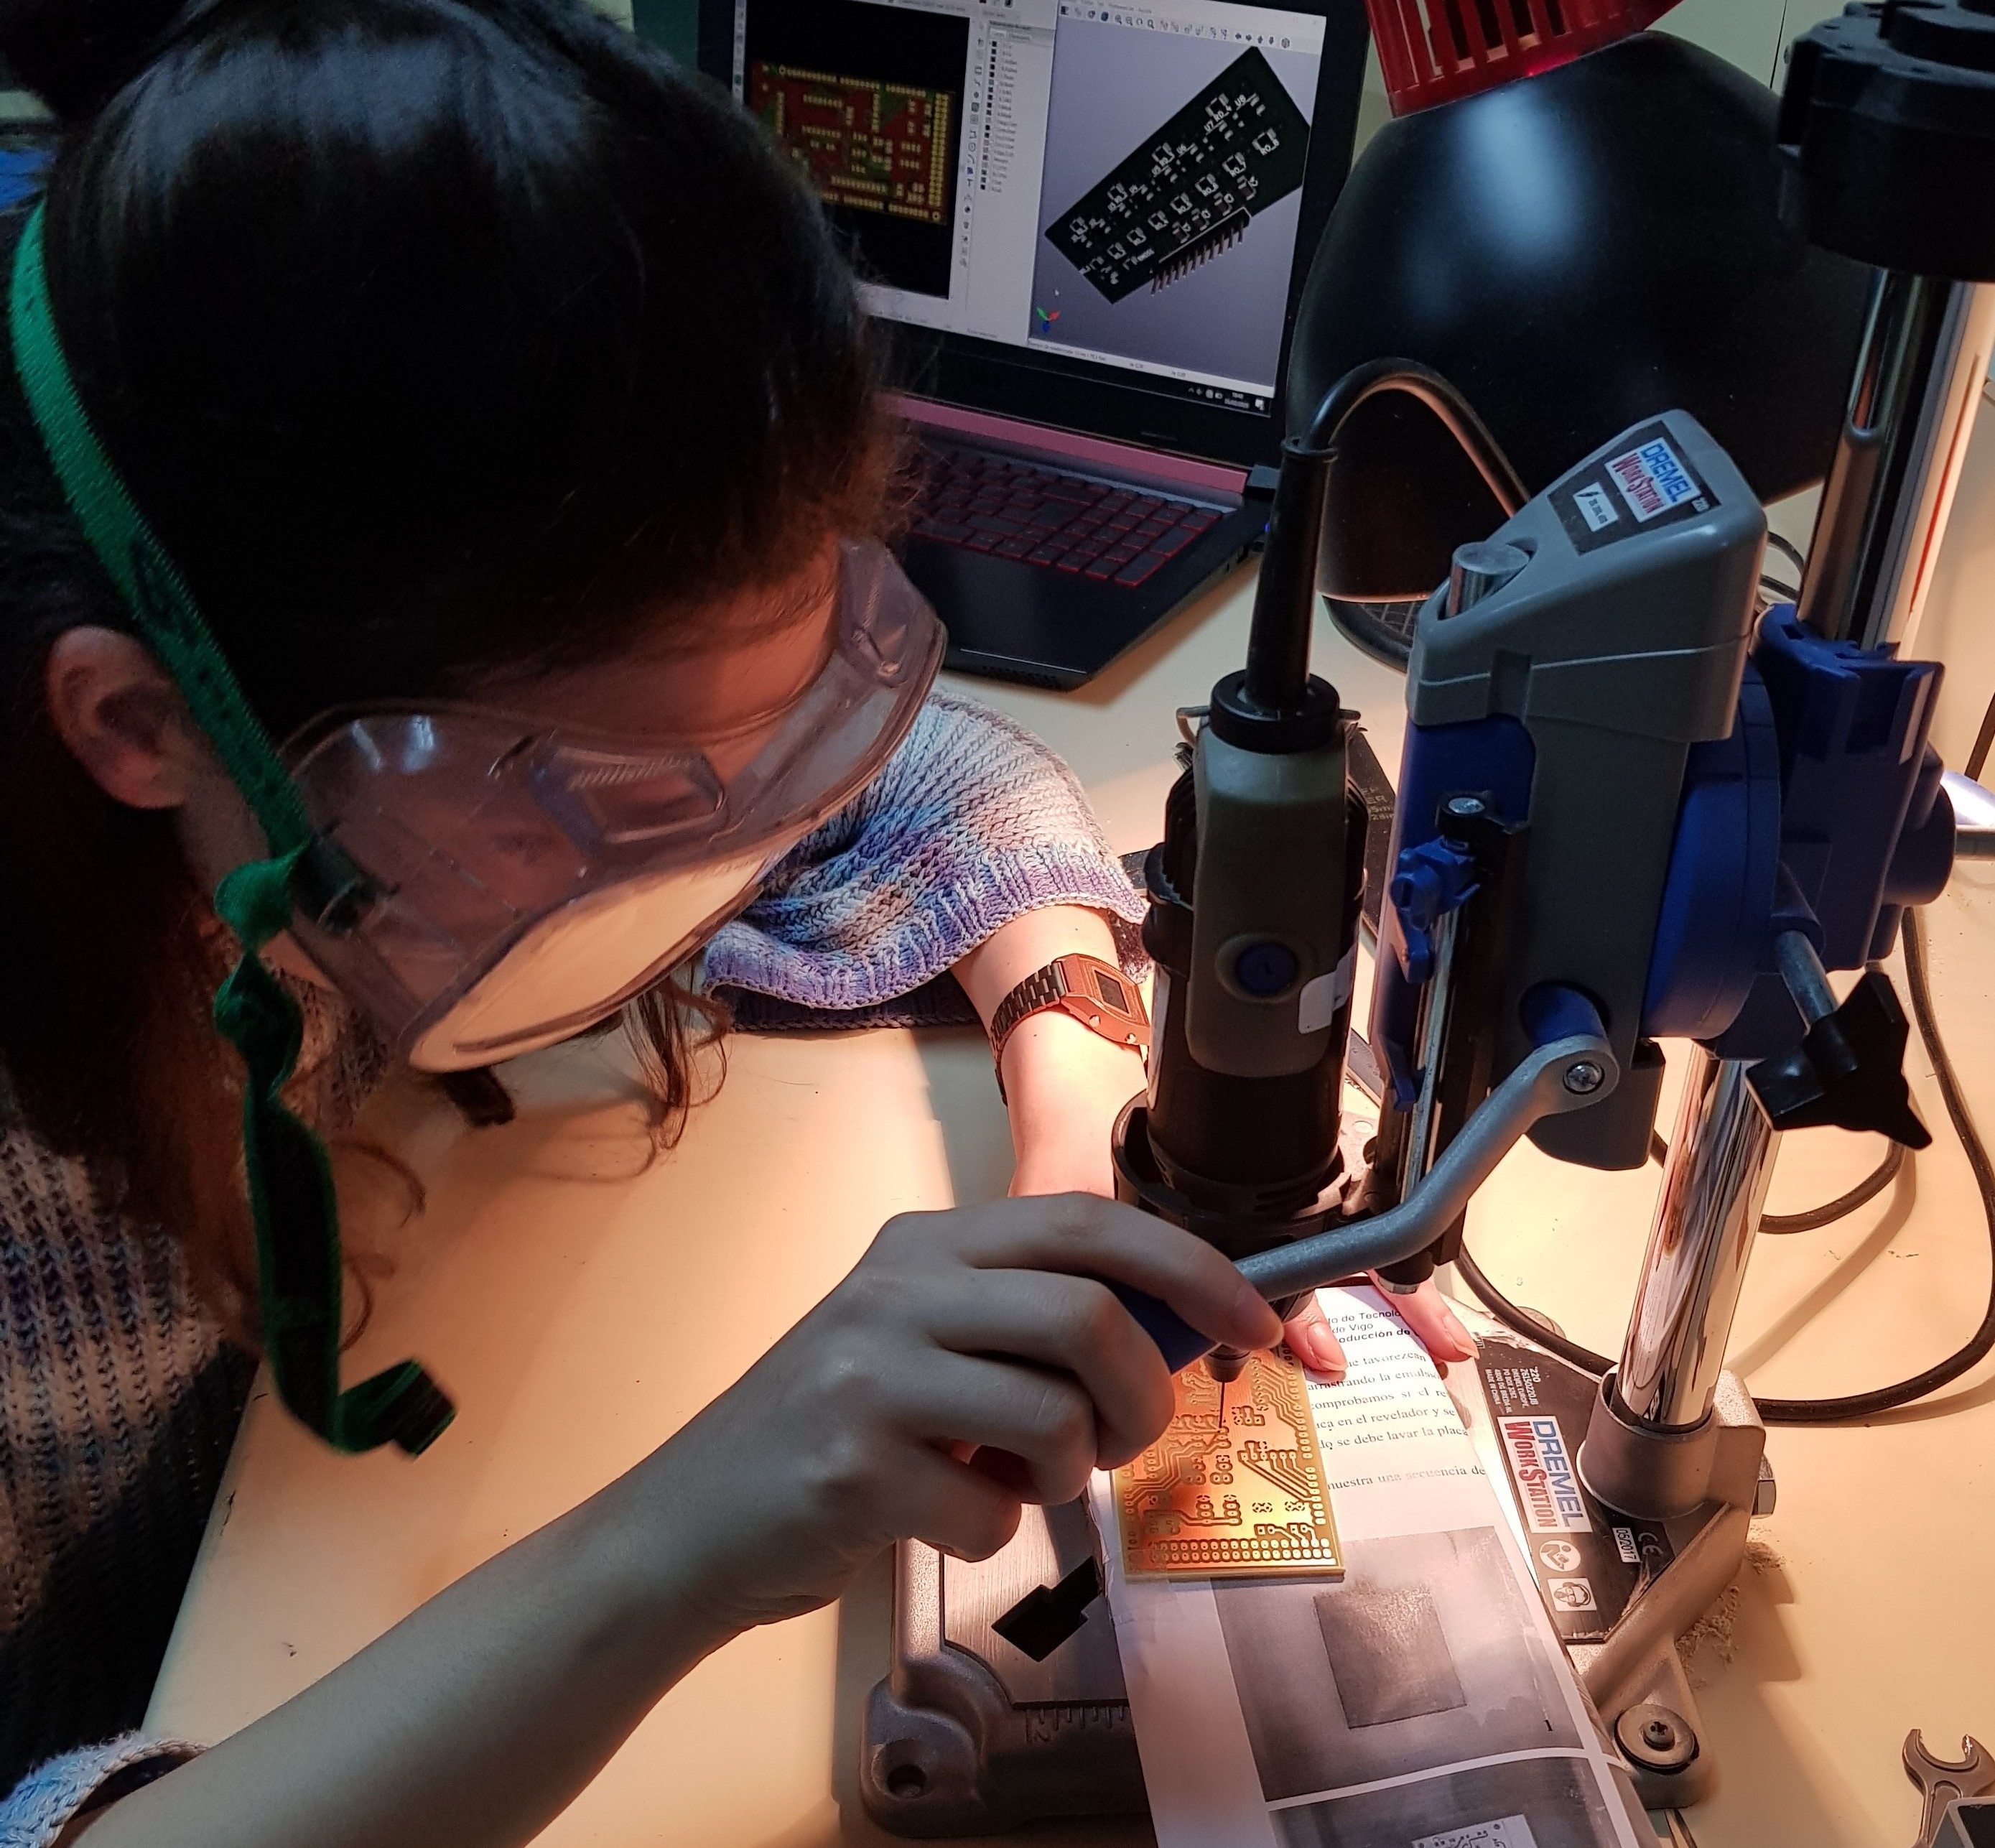
\includegraphics[width=.49\textwidth, height=\taladroHeight]{figures/process_drilling_team_elena.jpg}}
	\subfigure[Miguel hyper-drilling]{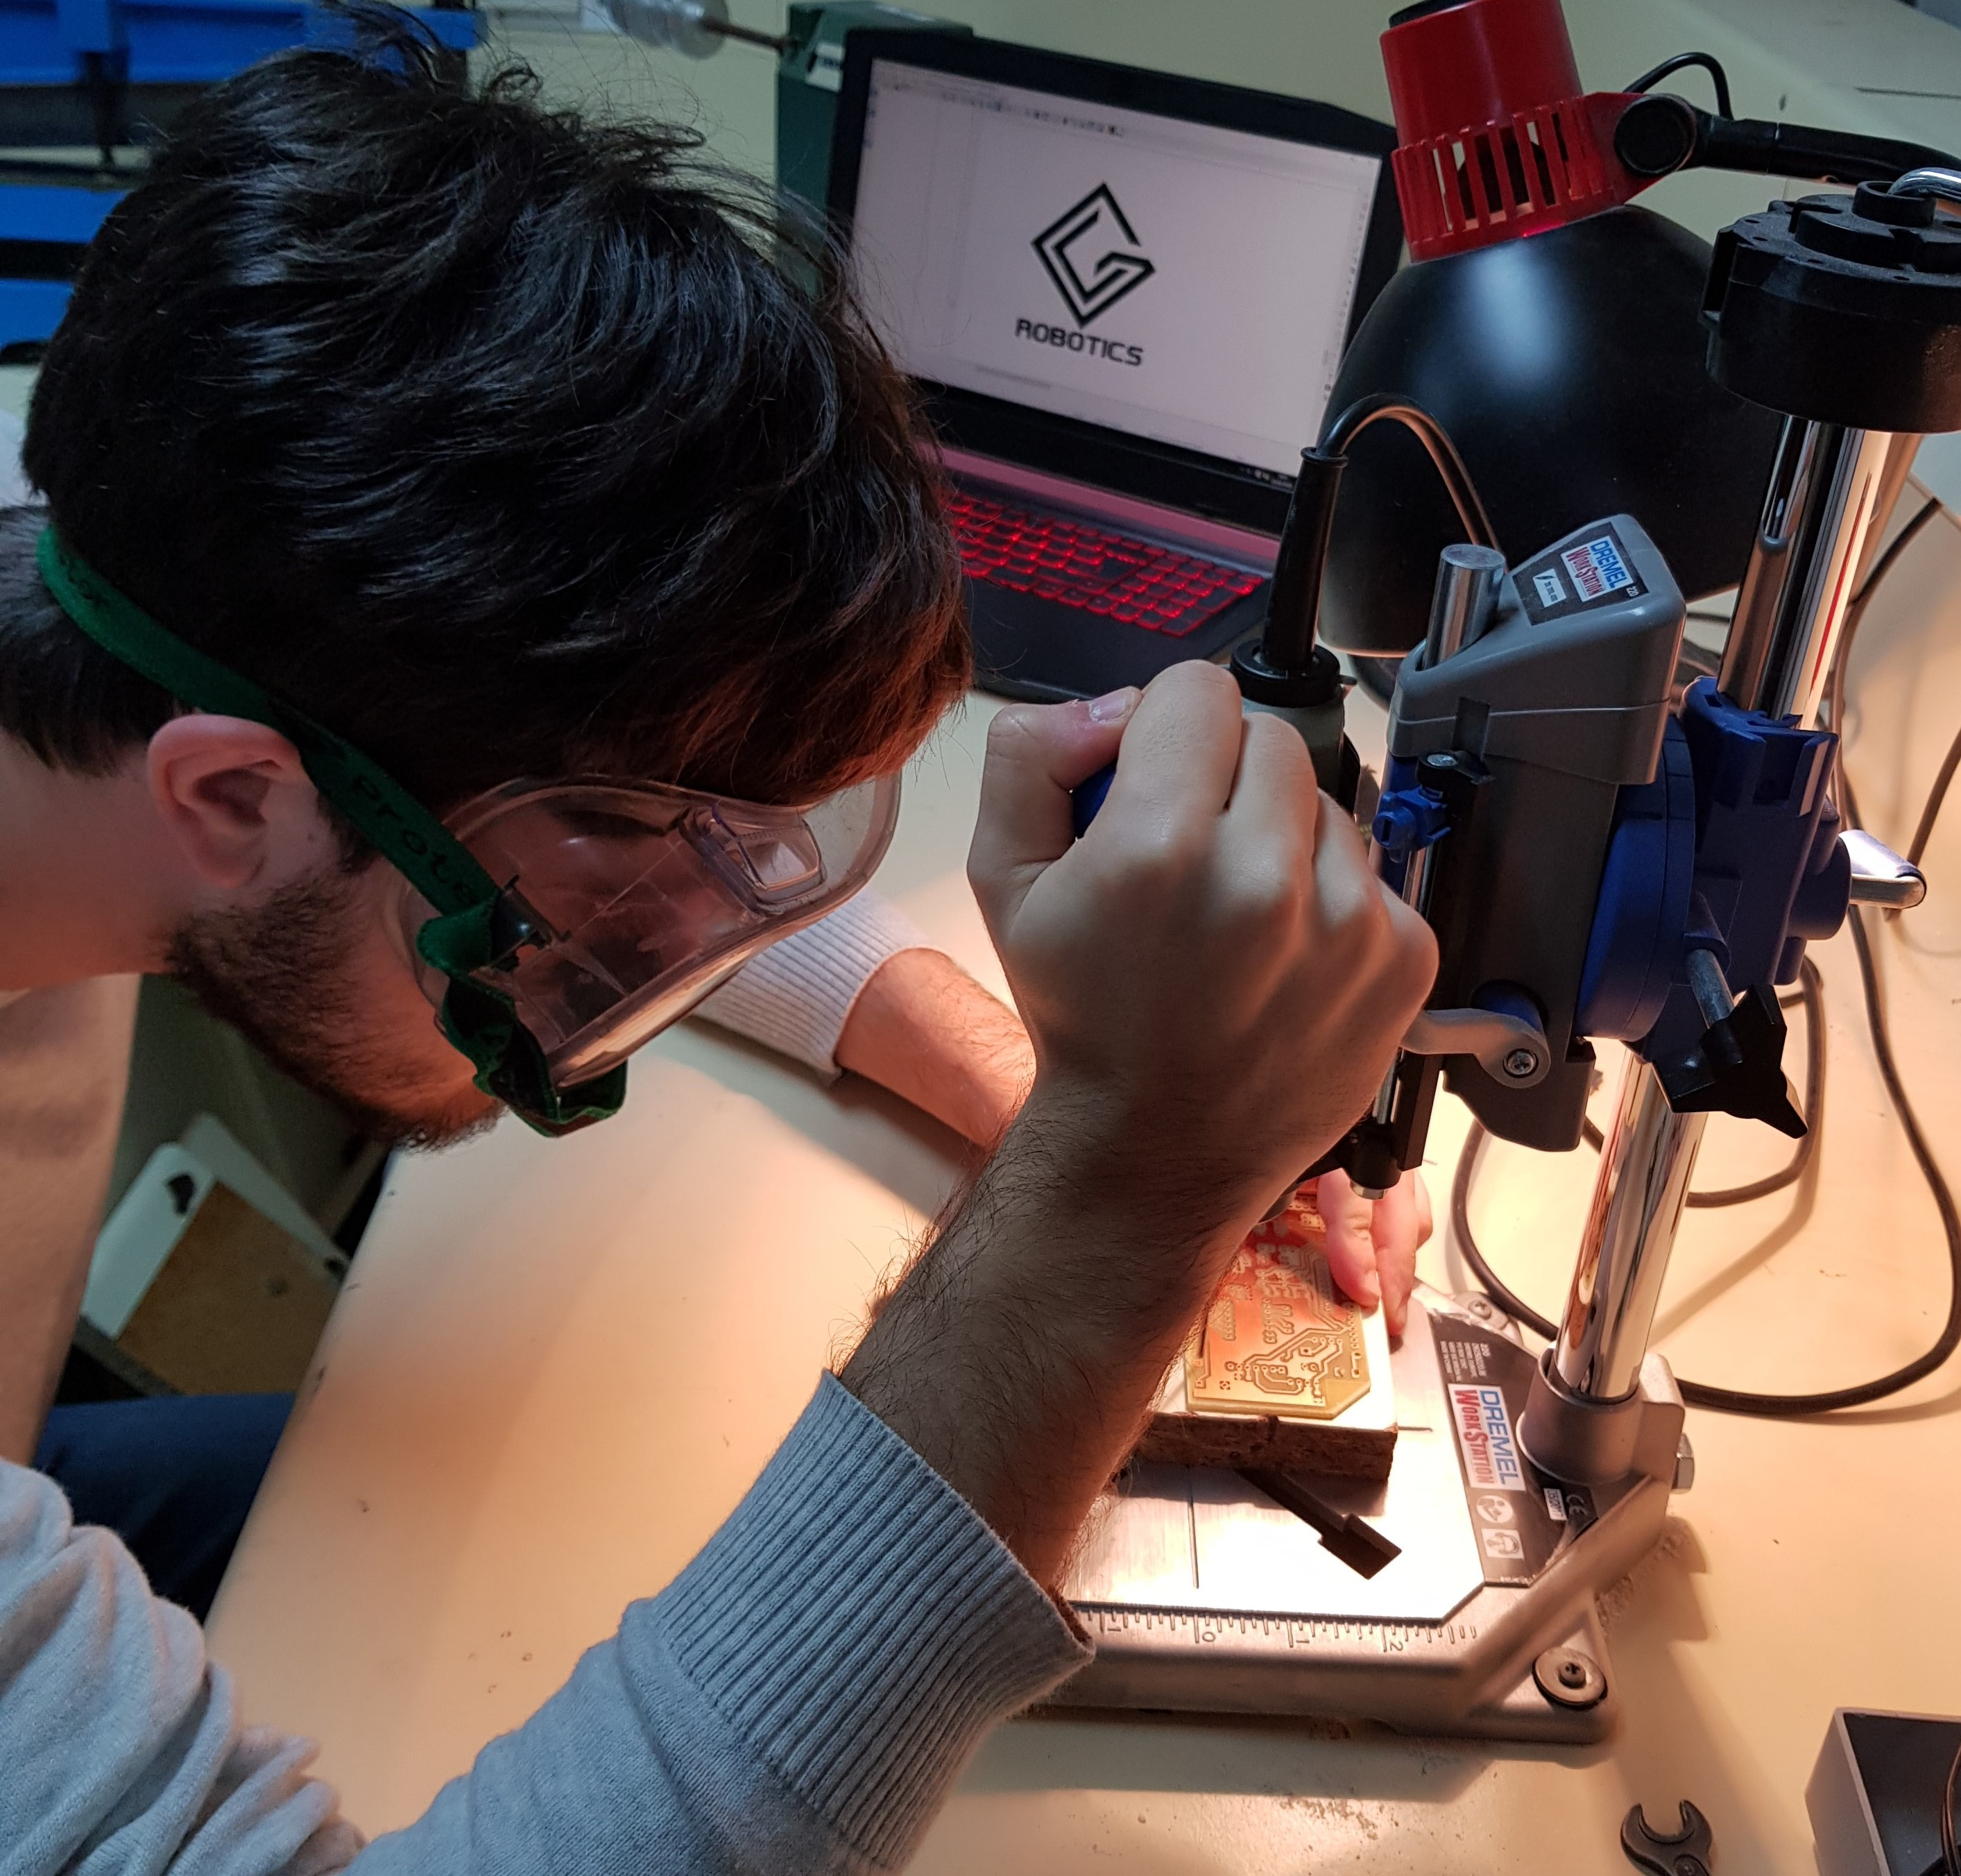
\includegraphics[width=.49\textwidth, height=\taladroHeight]{figures/process_drilling_team_miguel.jpg}}
	\subfigure[Fer flower-drilling]{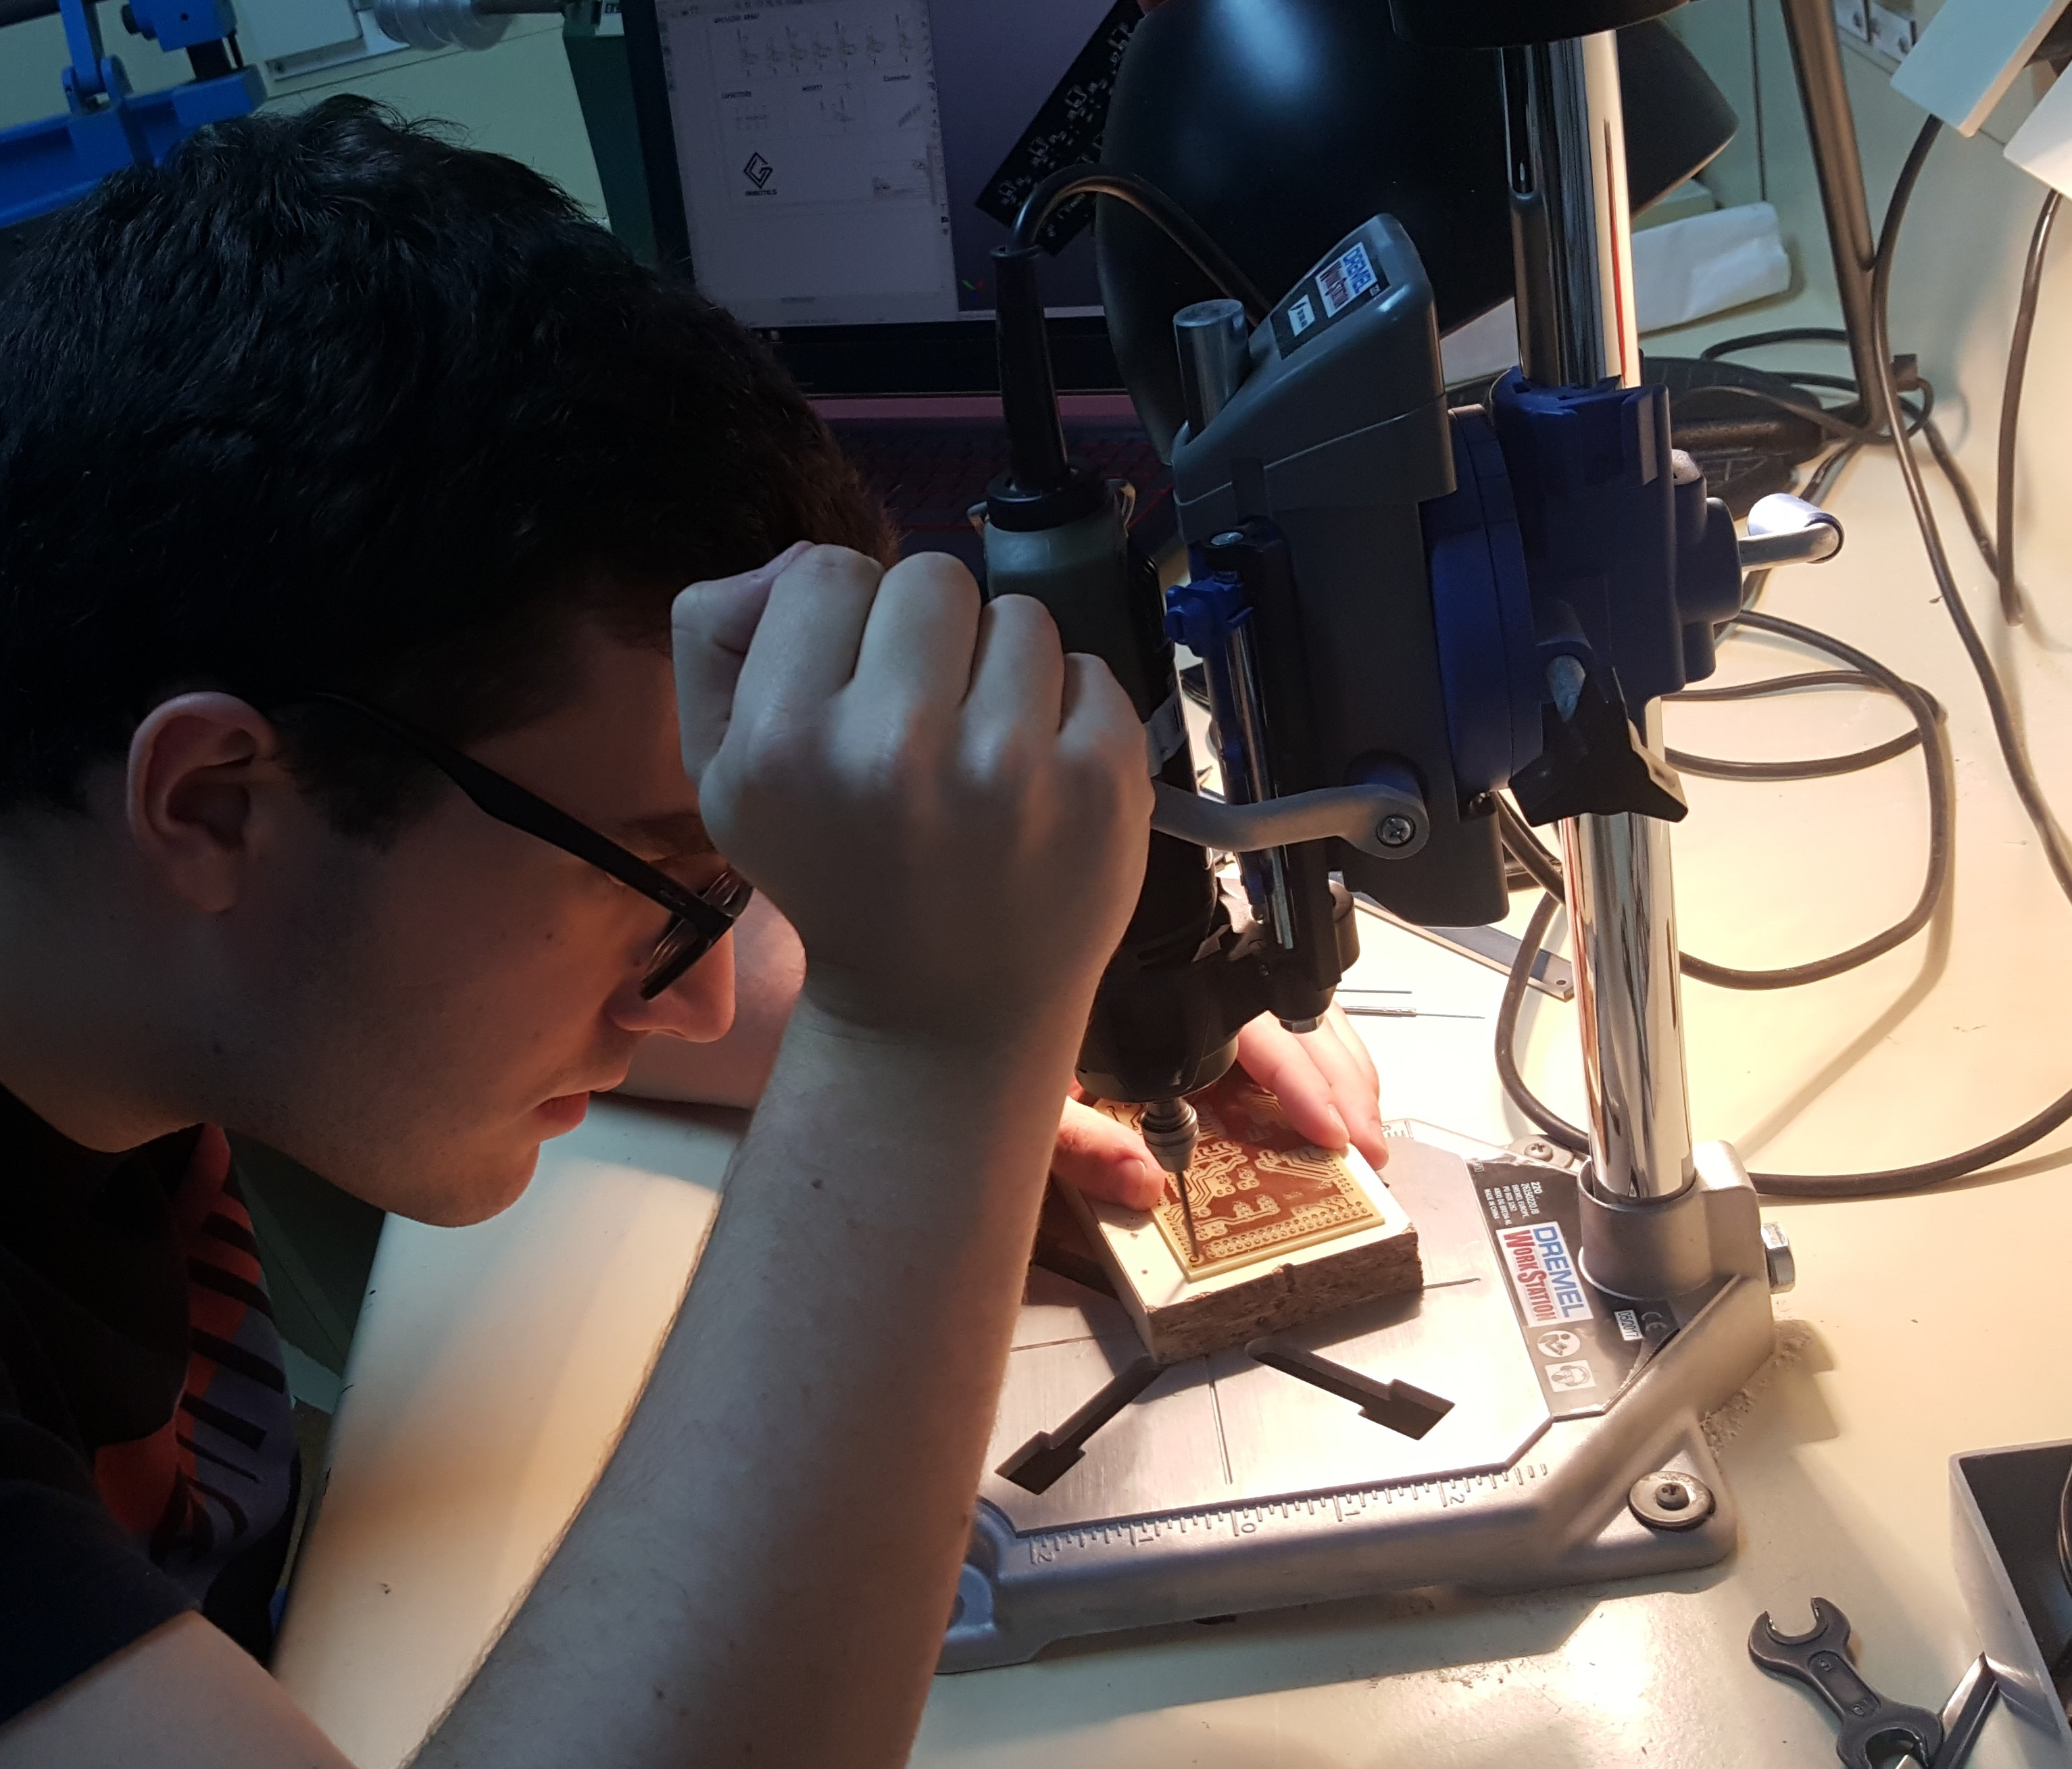
\includegraphics[width=.49\textwidth, height=\taladroHeight]{figures/process_drilling_team_fer.jpg}}
	\caption{Drilling examples with a fixed Dremel}
	\label{fig:drill}
\end{figure}
%
When this process is finished the PCB can seem like the PCB shown in the \autoref{fig:agujeritos}, in which only two diameters have been necessary.
%
\begin{figure}[H]
	\centering
	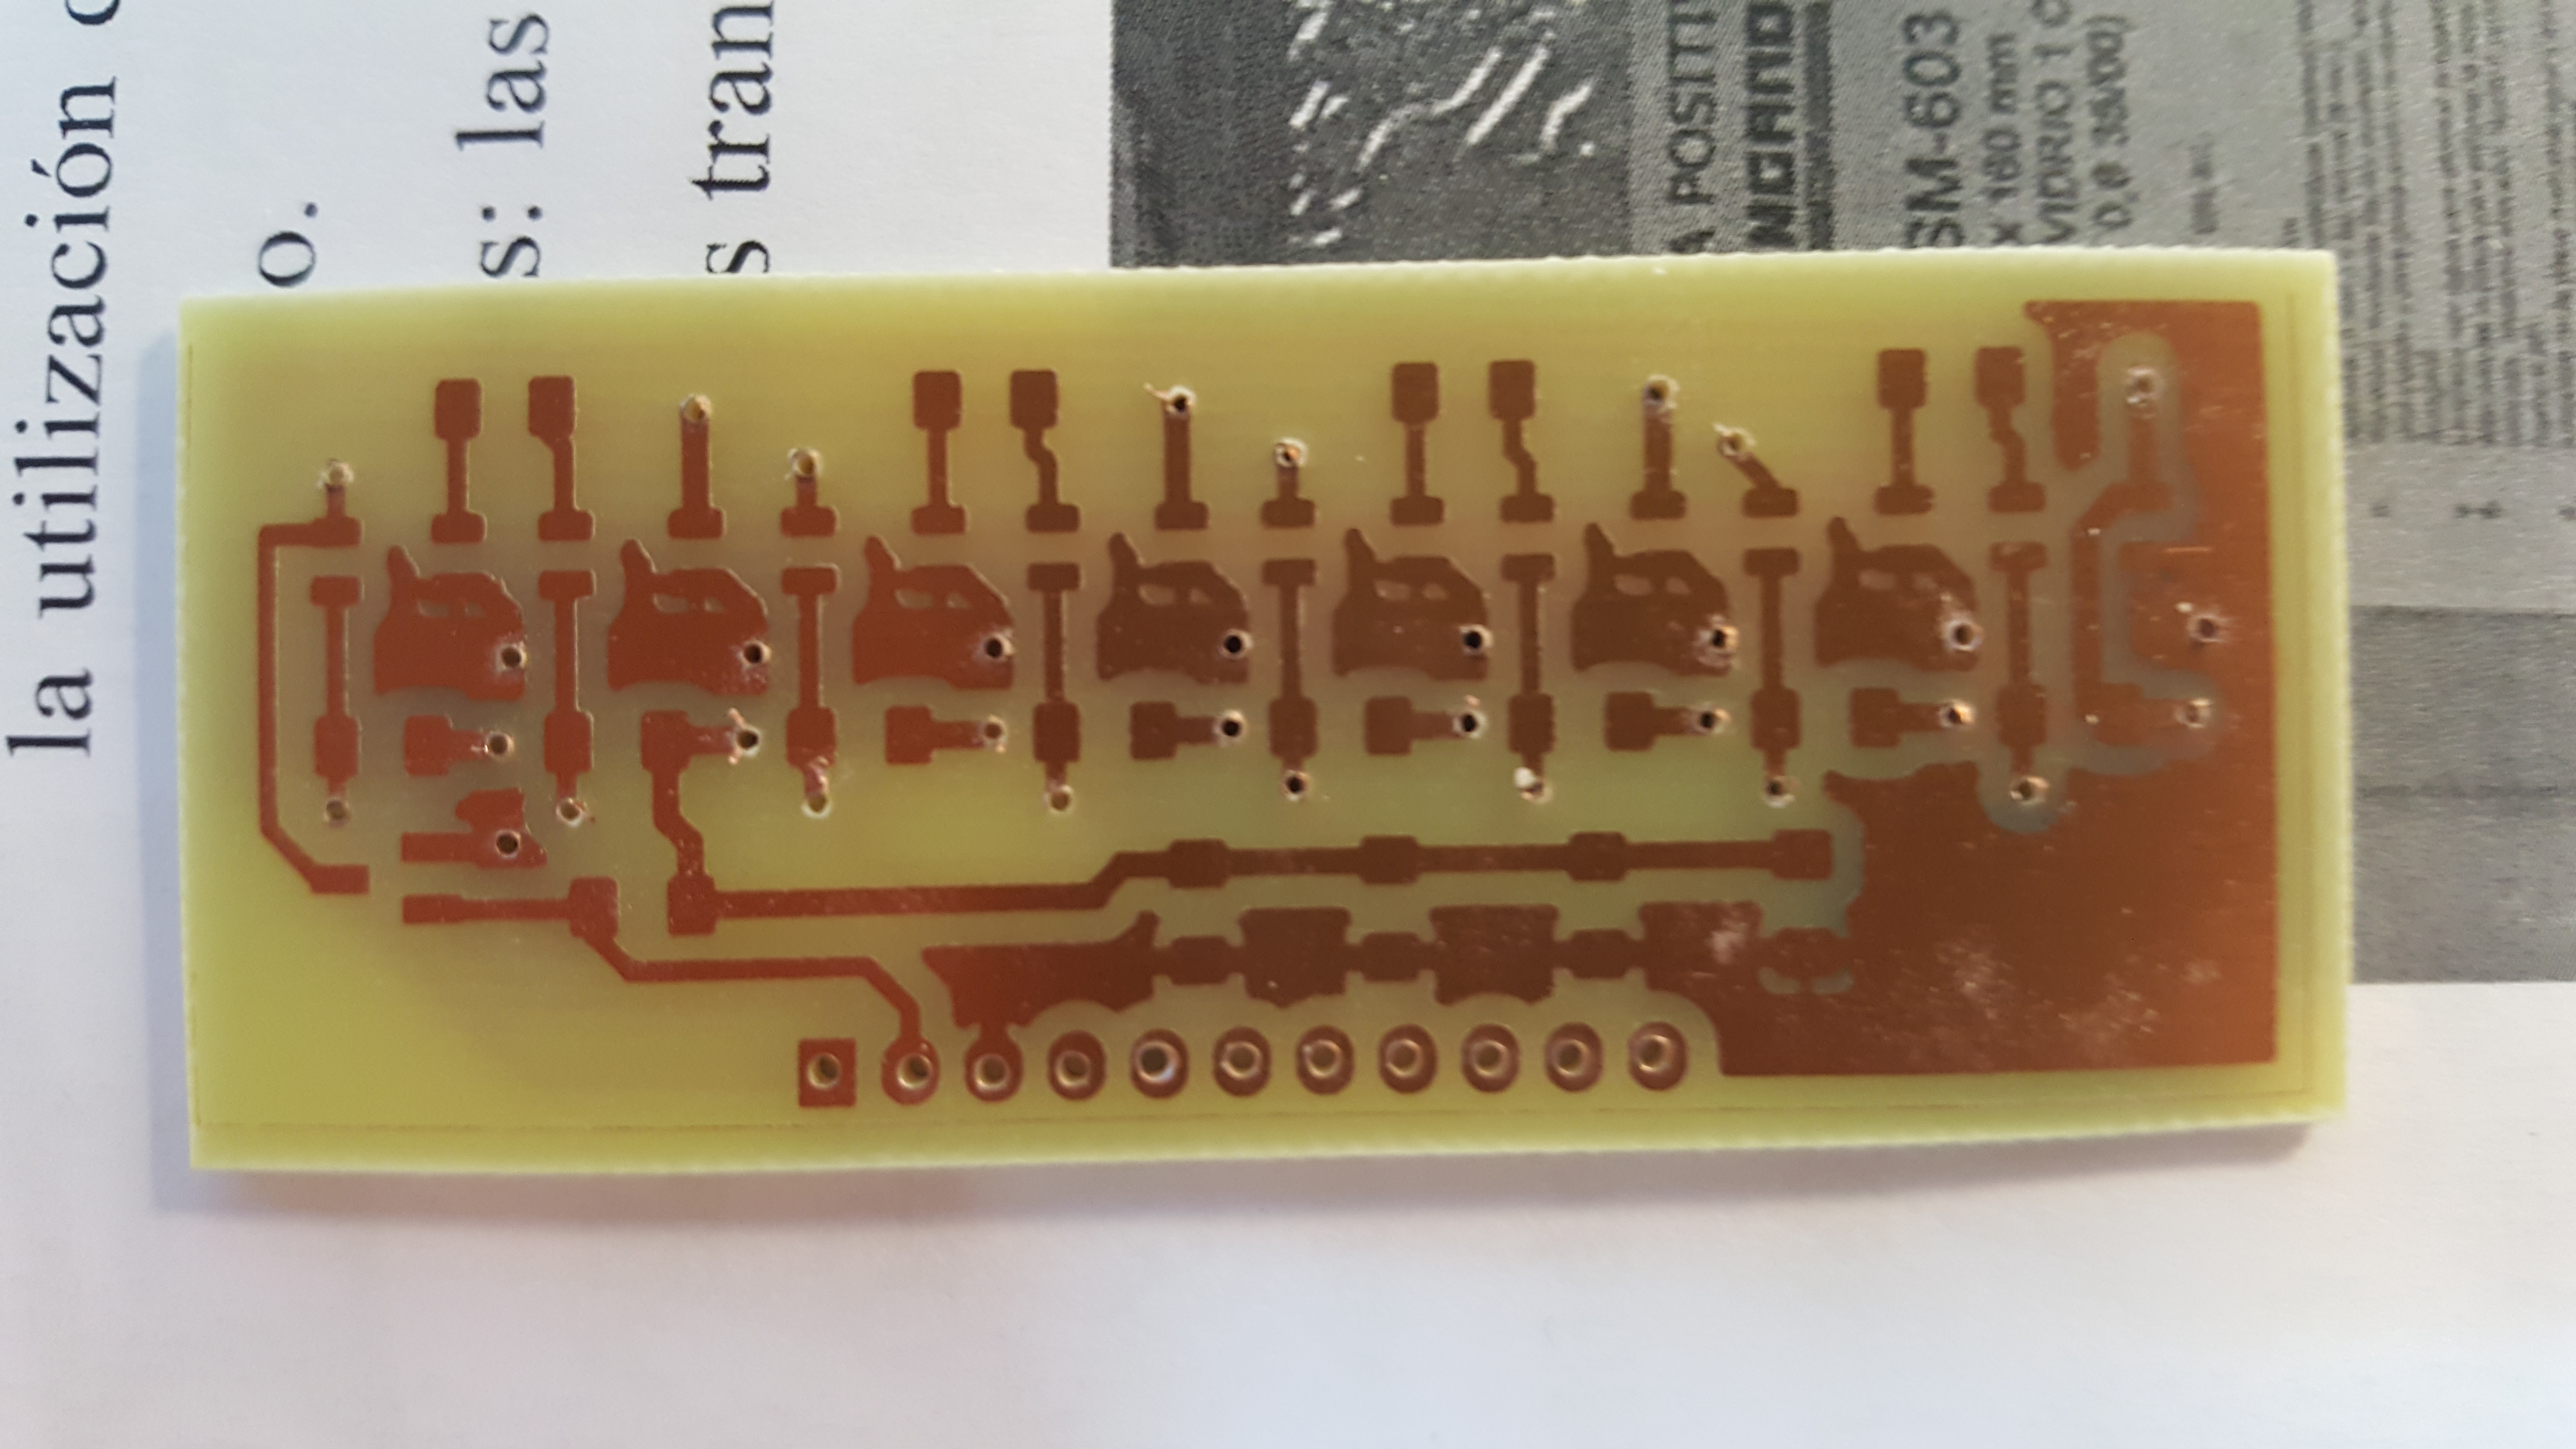
\includegraphics[width=.49\textwidth]{figures/pcb_result_drilled_holes.jpg}
	\caption{PCB drilled view}
	\label{fig:agujeritos}
\end{figure}
%
%
\section{Soldering}
%
After aaaaaaaall this steps only have to sold the components on the PCB. At this case, the components used in the PCBs of the \autoref{fig:pcbsmain} are THT and Surface Mounting Device (SMD). Remember using flux is recommendable in both cases. To end this long adventure use a special spray or transparent nail polish\footnote{There is some special sprays that can be used before solding because they allows to sold even with it} to protect te copper and avoi copper rusting.
%
\begin{figure}[H]
	\centering
	\subfigure[Solded PCB with SMD components]{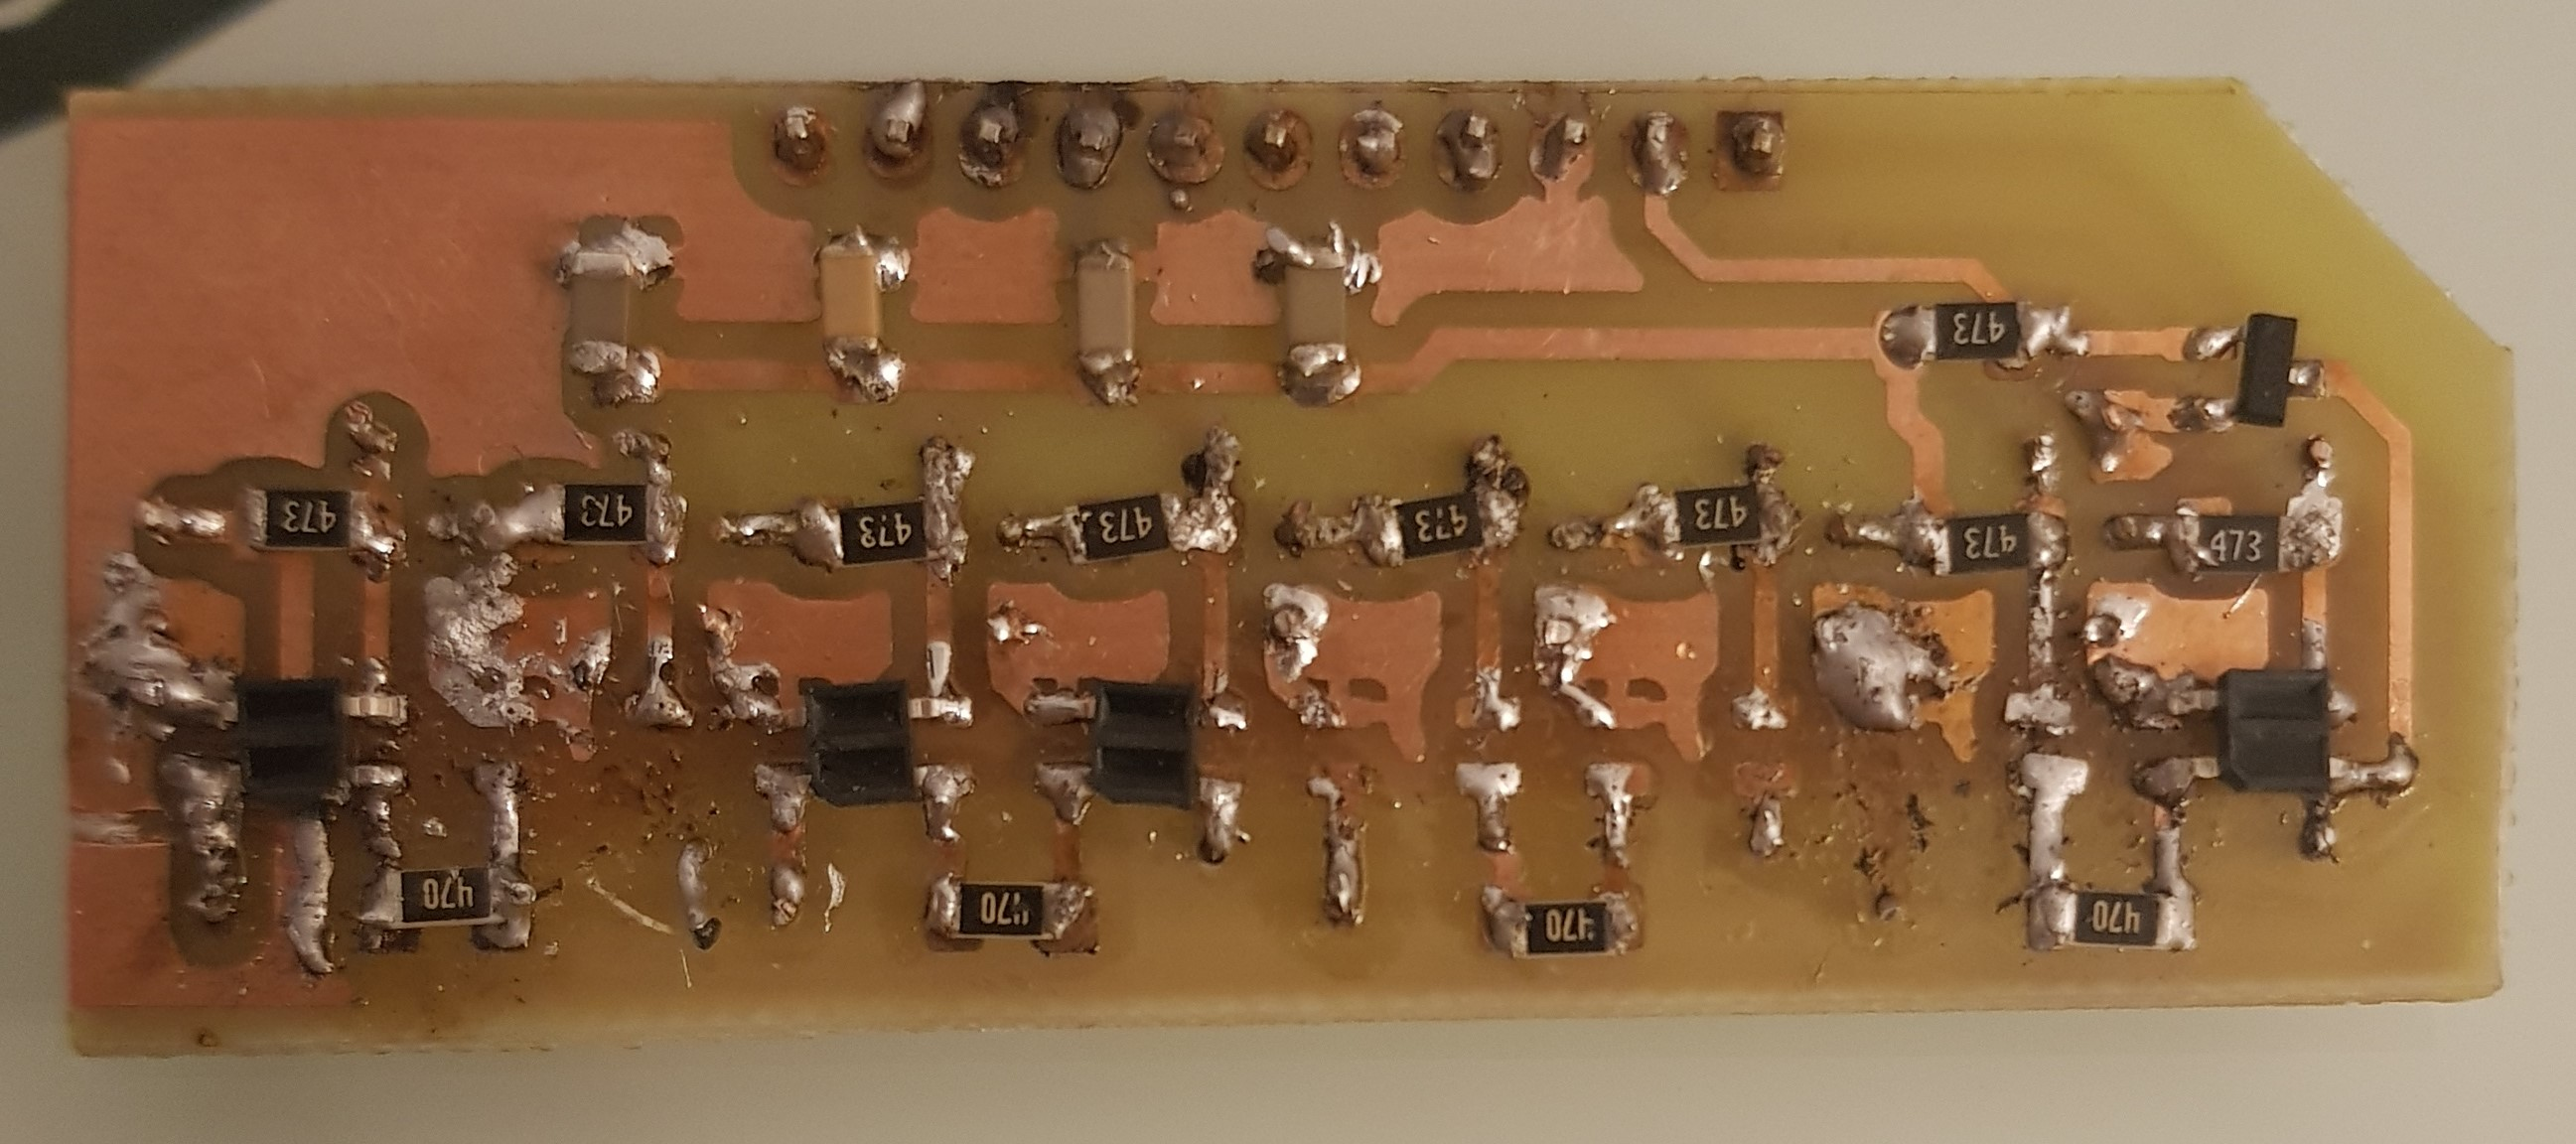
\includegraphics[width=.7\textwidth]{figures/pcb_result_soldered_smd.jpg}}
	\subfigure[Solded PCB with THT components]{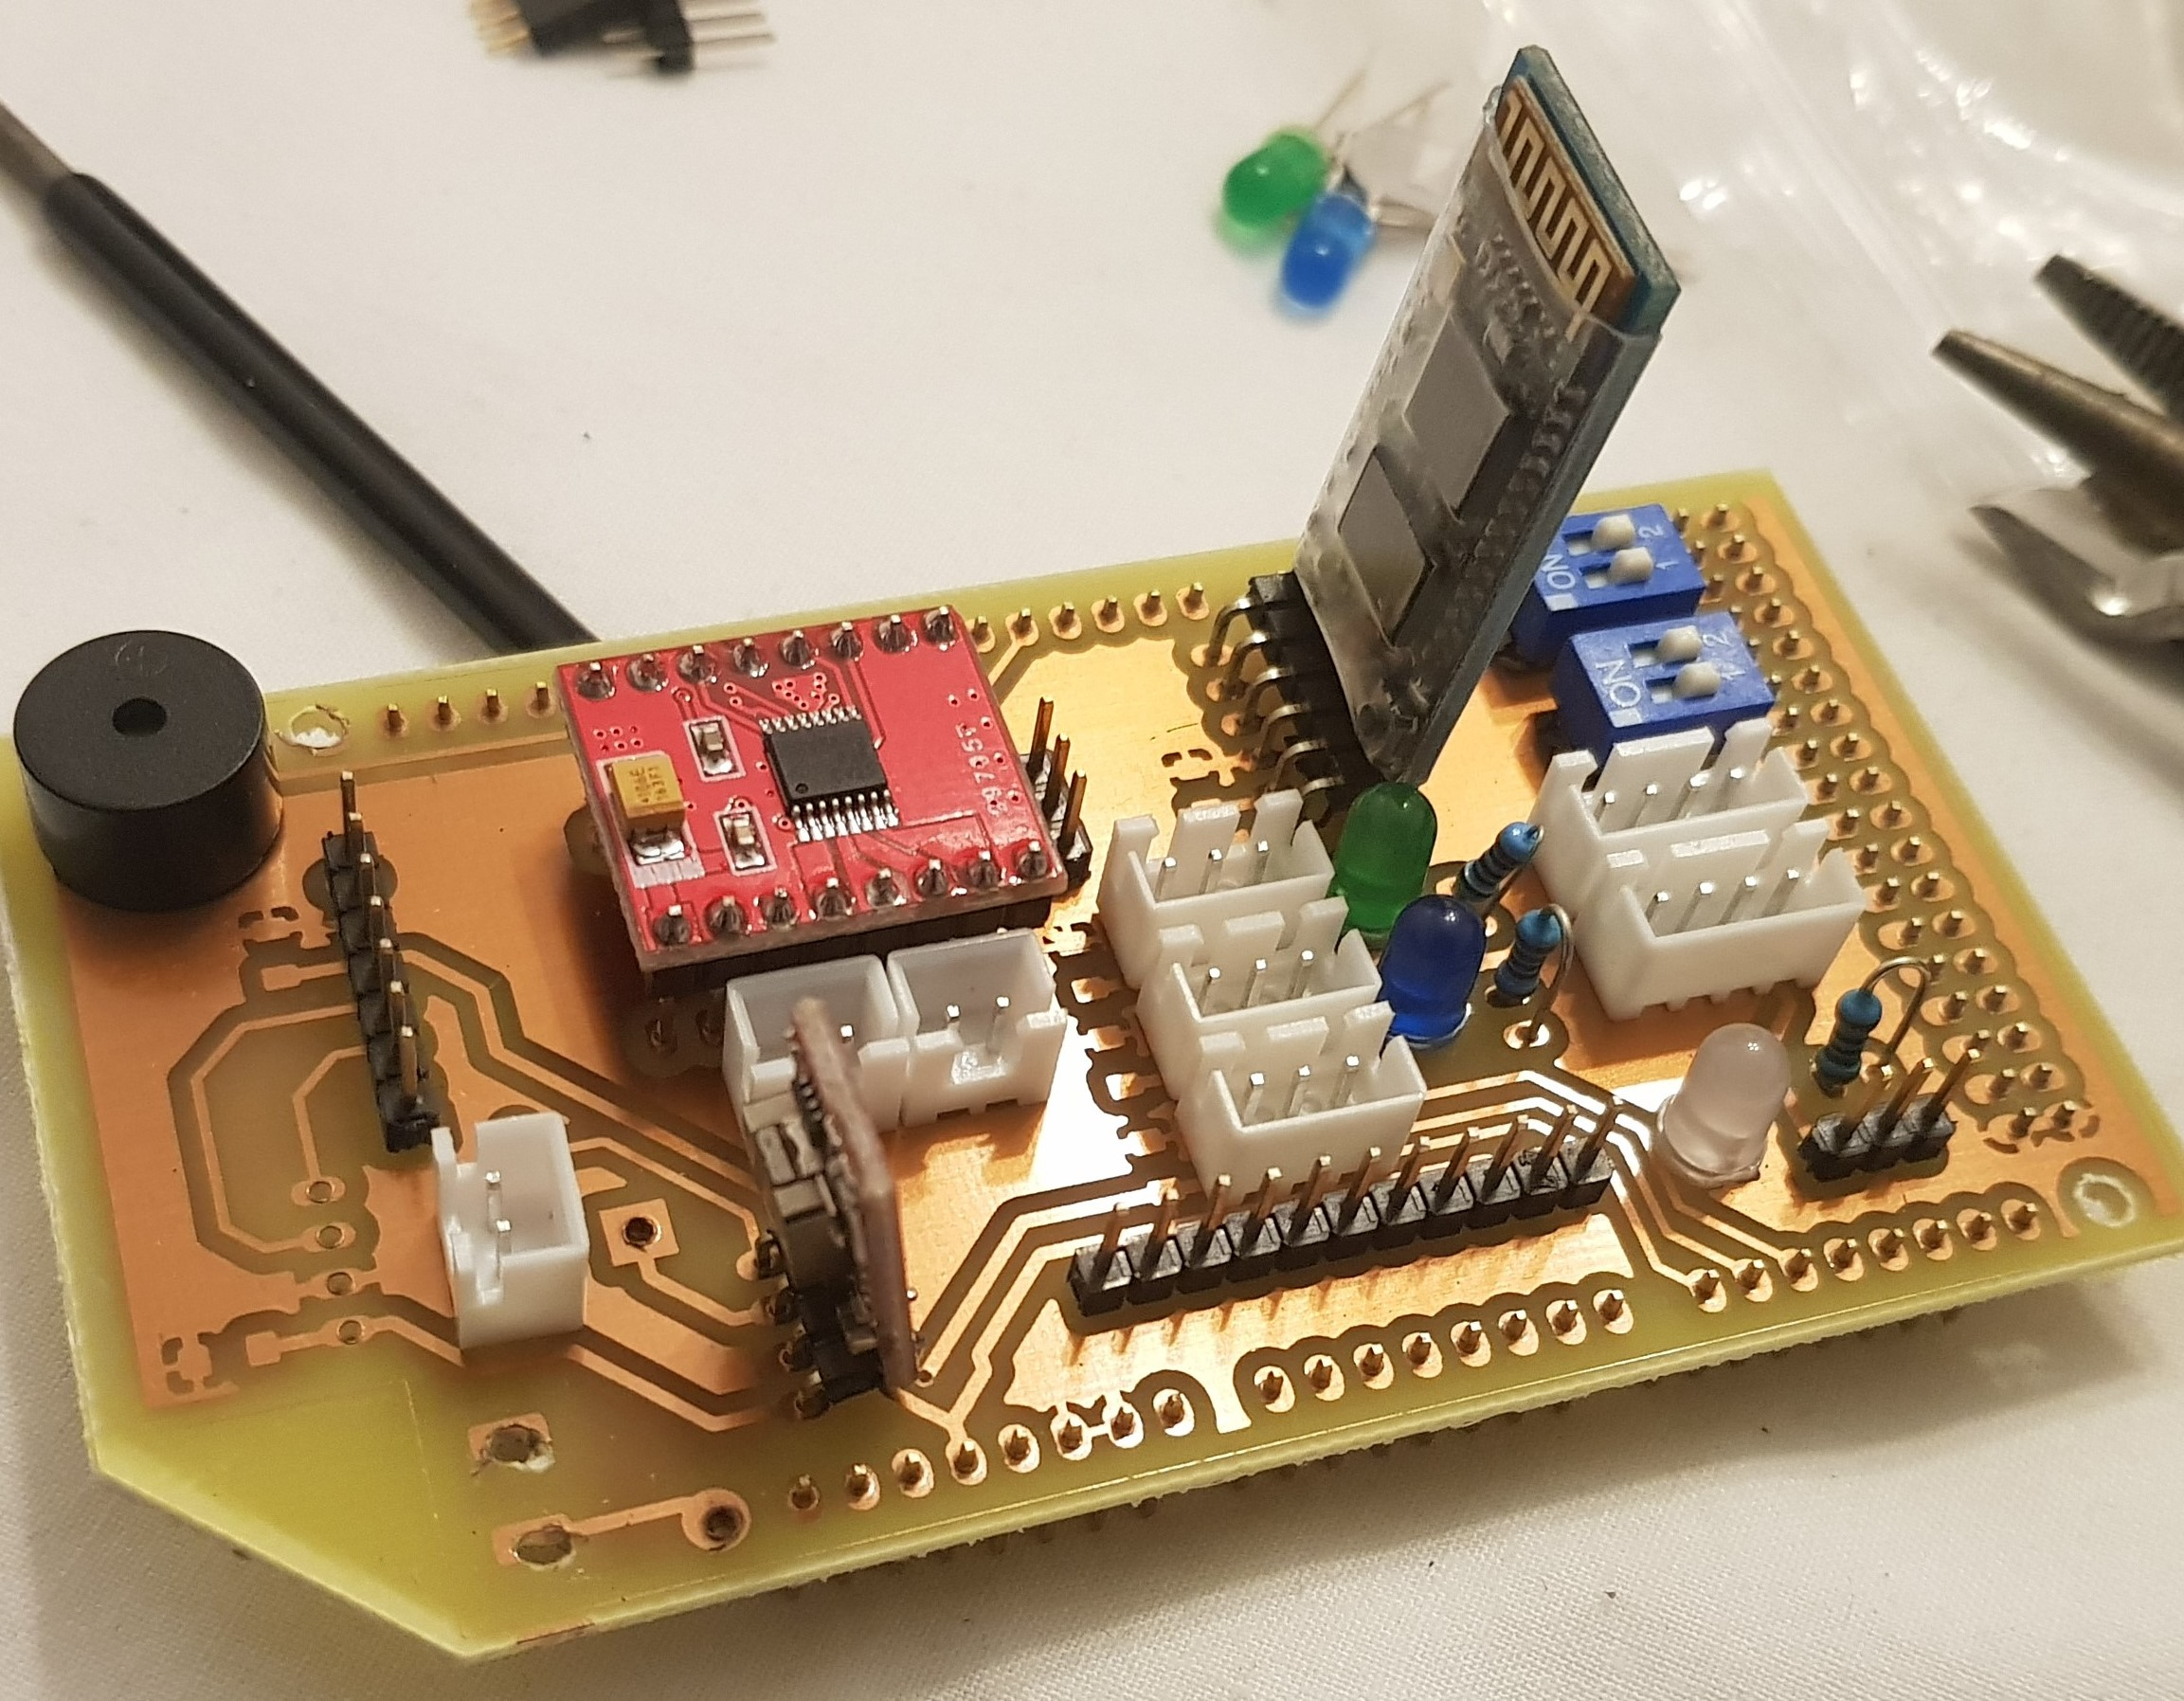
\includegraphics[width=.49\textwidth, height=\morepcbsHeight]{figures/pcb_result_soldered_tht.jpg}}
	\subfigure[Assembled PCB with THT components]{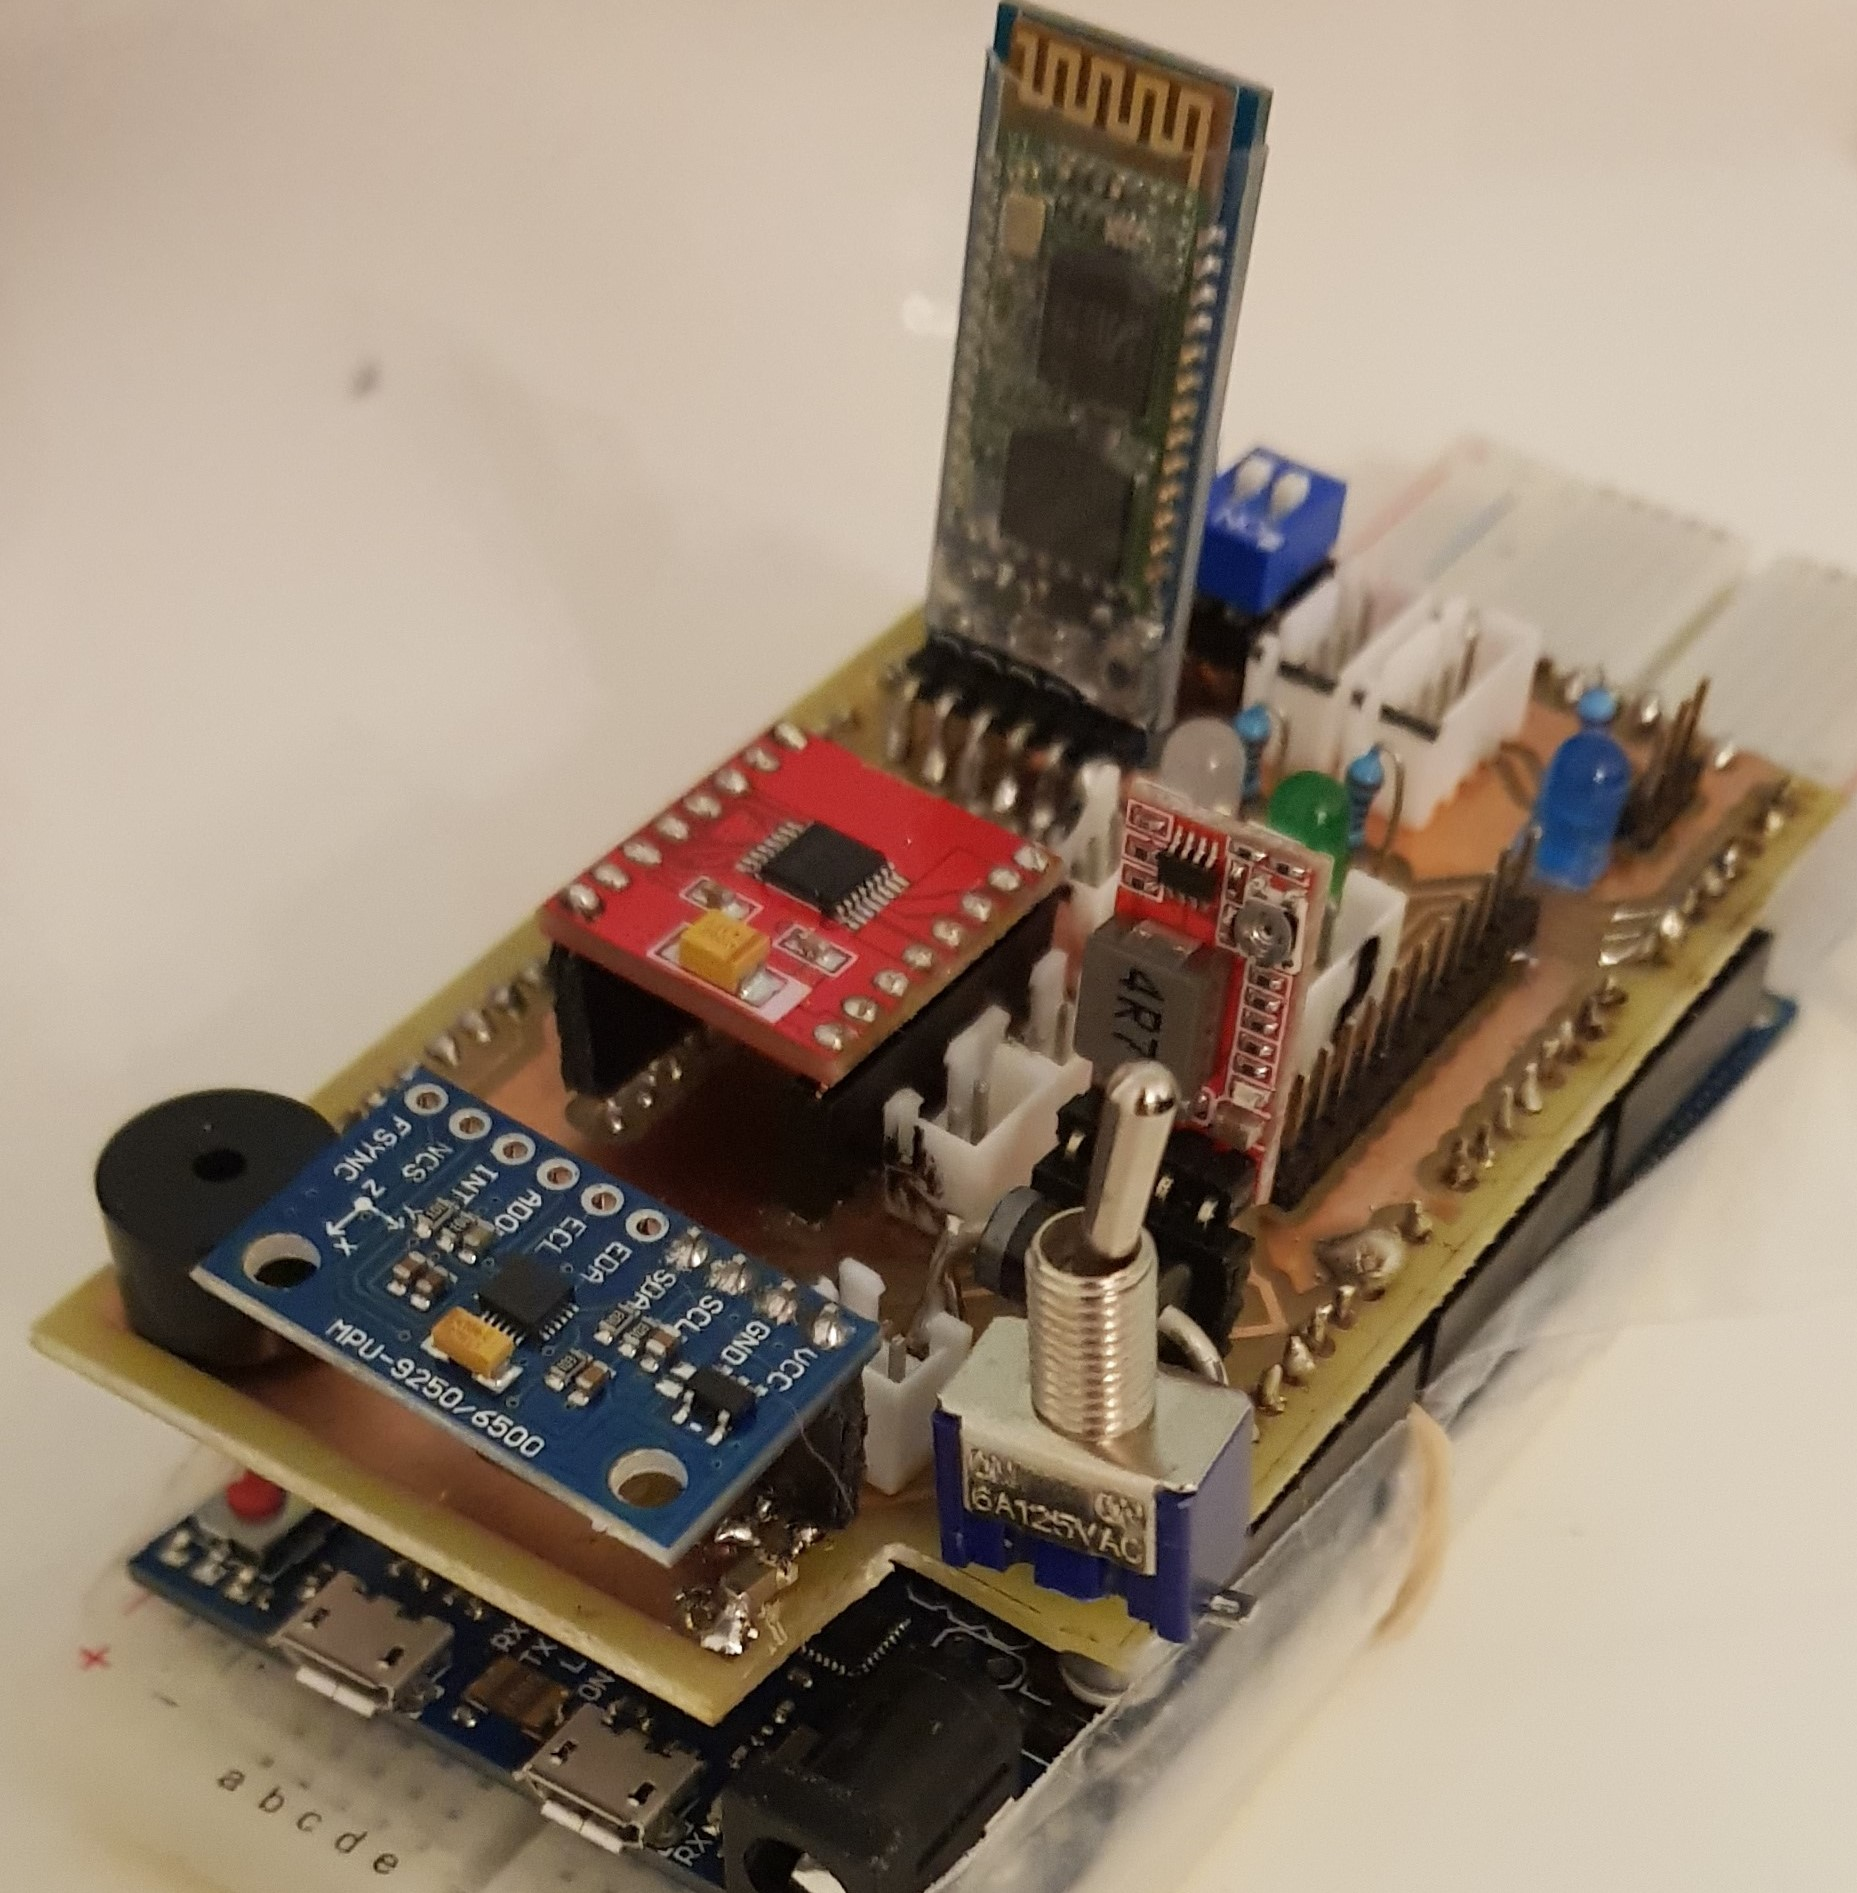
\includegraphics[width=.49\textwidth, height=\morepcbsHeight]{figures/pcb_result_assembled_tht.jpg}}
	\caption{Views of PCB solded and assembled with SMD and THT components}
	\label{fig:pcbsmain}
\end{figure}
	
\end{document}